%\chapter{Computations}
\chapter{Imaging a bubble influenced by a low frequency driving wave}\label{ch:mechanisms}


%The calculations of this chapter were performed with bubble++, 
%a templated c++-library designed and built by the author for the simulations carried out in this thesis.
%The library design and implementation is detailed in \appref{library}.


\section{Introduction}

Bubbles are generated at lower pressures at lower ultrasound frequencies (\chapref{nucleation})
but the resolution is poor for imaging.
To overcome this problem two ultrasound waves are used in this thesis;
the first, the {\em driving wave}, is used to generate the bubbles; 
the second, the  {\em imaging wave}, is a short pulse at a much higher frequency that is used for imaging.
The  lifetime of the generated bubbles can be short
and so the two waves are timed so that they are incident upon the bubbles simultaneously.
This means that although the driving pulse arrives first,
the imaging pulse arrives before the driving pulse has completed.
%The bubbles are therefore imaged as they are created.

The limited frequency response of ultrasound transducers usually necessitates that the pulses
are generated by two different transducers.
We assume that this is the case here.
The imaging wave therefore filters out most of the pressure generated by bubble in response to the driving wave.

However, the driving wave does still influence the remaining high frequency scatter.
It controls the phase-space%
\footnote{
  The phase-space of a bubble is comprised of the bubble radius, $a$, and the bubble wall velocity, $\dot a$.
  The phase-portrait is the two dimensional trajectory of  $a$ and $\dot a$ in phase-space.
}
trajectory of the bubble prior to the arrival of the imaging pulse.
The time  delay between the arrival of the two waves determines 
which portion of the phase-space trajectory is {\em sampled} by the imaging pulse.
The driving wave and the time delay can therefore be used together to manipulate the  radius and velocity
of the bubble when imaged. 
% to maximise its response to  a particular imaging pulse.
One immediate application of this is to temporarily shrink a conventional microbubble  so that it
may resonate at a higher frequency.

%Therefore, while the nucleation step requires the use of two waves in this thesis,
%imaging a bubble with two excitation pulses is a powerful technique even for preexisting bubbles.





%The driving wave, although not imaged directly,
%still exerts an influence  on the high frequency scattering of the bubble.
%It alters the pressure surrounding the bubble
%and in turn the bubble's radius and velocity.
%If the driving pressure does not change significantly over the duration of the imaging pulse,
%then it might be hoped that the driving wave can be understood purely as altering the boundary conditions of the bubble:
%the ambient pressure, and thereby the equilibrium radius,
%and the initial velocity of the bubble wall. % when imaged at higher frequencies.
%Unfortunately, this is only true for low amplitude driving waves,
%where the bubble responds approximately linearly to the driving wave;
%it does not in general follow that a small change in the driving pressure corresponds
%to a small change in the bubble radius and velocity.


%Non-linear effects become unimportant when
%the second order perturbations  to the pressure are small, 
%with 1\% accuracy is achieved when the perturbation is $10\%$ of the ambient pressure.
%At atmospheric pressure, this corresponds to a driving pressure of \unit{10}\kilo\pascal. 
%Pressures of \unit{10}\kilo\pascal\ are not nearly sufficient to generate bubbles.
%Our intuition (which is guided by linear processes)
%must therefore be carefully checked with the numerical computation.






%The pressure necessary to generate the bubbles is above \unit{...}\mega\pascal\ (\chapref{nucleation}).
%In \chapref{measurement} we saw 
%that at such pressures the bubble wall collapses at very high speeds for very short times.
%During these parts of the cycle 
%the radius of the bubble (as influenced by the driving wave)
%cannot be considered as being in equilibrium,
%and the change in the bubble wall velocity is not simply a boundary value change;
%both the radius and the velocity change greatly within the duration of the imaging pulse.
%The imaging pulse is not short in comparison to the imaging wave
%The influence of a high amplitude driving wave is therefore more complicated than
%when the driving wave is weaker.


This chapter studies the influence of the driving wave on the high frequency response of a bubble.
Our final application is to imaging the small (sub-micron) bubbles that have been created 
with the driving wave.
However, 
since the two wave technique is an important one,
we broaden our discussion to include micron sized bubbles and  a driving wave of more conventional (lower) pressures. 

The aims of the study are two fold.
The first is to understand how the high frequency response of the bubble depends upon the portion of the phase-space trajectory sampled by the imaging wave.
For this we study the following five parameters that influence the trajectory:
\ilist{
\item the frequency of the driving and imaging waves, $\frd$ and $\fri$, respectively,
\item the amplitude of the two waves, $\Ad$ and $\Ai$,
\item the radius of the bubble, $a$.
}
in addition to the temporal offset  between the arrival of the two waves. %phase of the driving wave sampled by the imaging wave, $\phi_d$ (see \secref{comp:phase}).
The second aim is to explore this  parameter space
to find the `optimum' parameters for imaging a nucleated bubble.
%It is only in this second section that we restrict the parameter space to consider nucleation only.



%\begin{sidetext}{suggestion}{Move the introduction chapter...}
%Other parameters could be included on this list.
%For example, the surface properties of the bubble %(such as the presence or absence of a shell)
%certainly influence the bubble's response.
%However,  varying such parameters shifts the investigation from the two wave technique
%into a study into the application of the technique to particular circumstances.
%For this reason we fix all of the properties of the bubble %(summarised in \tabref{})
%apart from the radius.
%A distribution of radii is inevitable in any bubble experiment, 
%and so this variable cannot be ignored.
%%}{Move the introduction chapter...}
%%
%
%Also relevant is the number of cycles of each wave.
%However, in this thesis we restrict our consideration to short pulses. 
%%we are interested only in short pulses in this thesis.
%We limit the duration of the driving wave to \unit{20}\micro\second,
%and the number of cycles of the imaging wave to 3.
%The imaging wave is considered to be the shortest that is realisable;
%the transducer will always ring making shorter waves impossible. 
%\end{sidetext}

 

This chapter begins by  detailing in \secref{comp:pulses}
the simple linear model used for the  incident pulses  in this chapter.
%We use a simple linear model.

Second, in \secref{comp:phase}, we distinguish the notions of phase that are used in this chapter:
the phase of the  driving pulse, $\phid$,
and the phase of the bubble's phase-space trajectory, $\phib$.
The latter is more physically relevant, 
the former we have better control over. 
The phase (driving or bubble) at which the incident wave arrives is denoted with a subscript 0,
that is $\phidi$ and $\phibi$, respectively.
%We find that the perturbation induced by the imaging wave in the bubble's trajectory
%is greater when the when the expansion caused by the imaging wave is not balanced by the contraction.
%It is greater, therefore, when the bubble is in its contraction phase when the imaging wave arrives,
%an observation confirmed in \secref{phase_amp}.


Third, in  \secref{comp:optimum},
we describe how we characterise the high frequency scatter that returns in two wave imaging.
To avoid imaging the higher harmonics induced by the driving wave   a two pulse technique is introduced.
First the bubble is imaged with  both the driving and the imaging wave and from this the response to just the driving wave is subtracted.
The result we call the {\em excess pressure}.
The {\em excess scattering cross section}, calculated from the excess pressure, is taken to be 
a measure of the effectiveness of the two wave technique.

With these preliminaries completed we consider in \secref{comp:examples} how the excess scatter
varies with the sampled driving phase, $\phidi$.
We confirm the behaviour that would be expected:
that a bubble that is smaller than its resonant radius (given the imaging frequency and amplitude)
has a stronger scatter when it is grown by the driving wave
and that a bubble that is larger than its resonant radius scatters more strongly when it is shrunk;
that the phase relationship with $\phid$ breaks down when the 
bubble starts to resonate under the influence of the driving wave,

Finally in \secref{comp:montecarlo} we explore the full  parameter space 
to find the `optimum' values of the driving and imaging pressure, frequency, 
and the phase $\phidi$ for imaging a \unit{100}\nano\metre-radius bubble.
In choosing this radius we are restricting our attention to the nucleation application.
To explore the parameter space Markov-chain random walk is employed.



In this chapter all bubbles are modelled with the acoustically-measured-Keller-Miksis equation.
The gas within the bubbles is assumed to be air and obey adiabatic thermodynamics.
The surrounding medium is modelled as water and the dynamic viscosity for the water-gas interface
is taken to be  \unit{$1\times10^{-3}$}\pascal\second.
Since we are interested in nucleated bubbles no encapsulating shell is modelled,
with an air-water surface tension of  \unit{0.07280}\newton\reciprocal\metre.
The ambient pressure $p_0$ is taken to be \unit{0.1013}\mega\pascal.
%This also frees our discussion from the larger parameter space that such details necessitates.
The parameters, unless otherwise stated, will take their values from \tabref{Param:Defaults}

\ctable[cap     = Parameter values unless otherwise stated,
        caption =  Parameter values unless otherwise stated,
        label   = table:Param:Defaults,
        pos   = h,
        %width = 0.6\textwidth,
        left
       ]
       {llcrc}
{
%\tnote{Where $m$ indexes the central cycle in the driving pulse.}
\tnote{The number of driving cycles depends on the frequency.
  It is chosen to be the first integer  number complete  after a duration of \unit{20}\micro\second.}
}{\FL
    &         &   &  Default &
    \ML
    &driving frequency &$\frd$  & \unit{0.5}\mega\hertz &
    \NN
    &imaging frequency&$\fri$ &        \unit{20}\mega\hertz   &     
    \NN
    &driving amplitude&$\Ad$ &        \unit{0.1}\mega\pascal   &    
    \NN
    &imaging amplitude&$\Ai$ &        \unit{0.5}\mega\pascal   & 
    \NN
    &driving cycles& &       \unit{20}\micro\second\tmark  &    
    \NN
    &imaging cycles& &        3  &     
      \LL
}

We restrict the imaging wave to short pulses of 3 cycles.
This is considered to be the shortest - and therefore with the greatest resolution -  that is realisable;
transducer ringing making shorter waves impossible. 
%The short pulse maximises the resolution.

We want the driving wave to be able to set up a near stable phase-space trajectory for the bubble.
This requires, in our experience, at least 5 or 6 cycles.
Long pulses are no good for over many cycles the wave will substantially change the bubble 
through processes such as rectified diffusion (which are not modelled).
We therefore limit the duration of the imaging pulse to be the shortest pulse greater than \unit{20}\micro\second\
with an integer number of cycles.
%Such pulses, additionally, can generally be generated by conventional imaging transducers.
%The heat generated in such timescales not being too great.

\subsection{The incident pulses}\label{sec:comp:pulses}


\begin{figure}[h]
 \centering
 \subfloat[driving pulse]{
   \label{fig:comp:pulses:driving}
   \includegraphics{c4_driving_wave.0}}
 \subfloat[imaging pulse]{
   \label{fig:comp:pulses:imaging}
   \includegraphics{c4_imaging_wave.0}}
 \subfloat[combined pulse]{
   \label{fig:comp:pulses:both}
   \includegraphics{c4_both_waves.0}}
  \caption{
    Examples of the incident pulses used in this thesis.
    The lower axis is the time at which a bubble experiences the incident wave.
    The upper x-axis is the phase of the driving wave.
    In  \subref{fig:comp:pulses:imaging} it is seen that the peak negative pressure of the incident wave
    occurs at the phase of $10\pi$.
   % The driving frequency used is \unit{2}\mega\hertz.
  }
 \label{fig:comp:pulses}
\end{figure}

The model used for the  driving and imaging pulses in this thesis is kept simple.
The waves are assumed to be linear sinusoids that are tempered
into finite durations with a half-wavelength cosine.
The first and last quarter are tempered,
with the middle 50\% being pure sinusoid.
A few examples are shown in \figref{comp:pulses}.



It would be possible to include greater complexity into the incident sound waves.
For example, including non-linear propagation of the pulse from the transducer to the bubble
would perhaps improve the correspondence with experiment.
However, including such complexities only serves to  hide the current investigation of two wave imaging 
within a huge parameter space.
We feel that a cosine-modulated sinusoid
is the simplest yet still plausible model for an ultrasound pulse.

\subsection{The word {\em phase} in this thesis}\label{sec:comp:phase}


In this thesis we refer to two different phase angles:
the phase of the driving wave, $\phid$, and the phase of the bubble's pulsation, $\phib$.

%The phase of the driving wave, $\phi_d$ is simply the phase of the underlying sinsoid of the 
The driving pressure is a modulated sinusoid  and $\phi_d$ is simply the phase of the underlying sinusoid
with respect to a cosine-wave.
It is shown on the upper axis to the plots in \figref{comp:pulses}.

%The driving phase therefore indicates the stage of the driving pressure 
%The driving phase is interesting because it indicates the  pressure generated by the driving wave that is sampled by the imaging pulse.
%When a short imaging pulse is incident on a bubble at the same time as the driving pulse,
%the driving-phase indicates where in the cycle of the driving pulse the imaging pulse arrived.
%Four different phase relationships are drawn in \figref{driving_phase}.


%\subsubsection{The bubble's phase, $\phi_b$}

\begin{figure}
  \centering
  \subfloat[\unit{10}\kilo\pascal]{
    \label{fig:Phases:small_phasor}
    \includegraphics{c4_phase_defn_linear_phasor.0}}
  \quad
  \subfloat[\unit{10}\kilo\pascal]{
    \label{fig:Phases:small_phase}
    \includegraphics{c4_phase_defn_linear_phase.0}}
  \\
  % \centering
  \subfloat[\unit{125}\kilo\pascal]{
    \label{fig:Phases:large_phasor}
    \includegraphics{c4_phase_defn_harmonic_phasor.0}}
  \qquad
  \subfloat[\unit{125}\kilo\pascal]{
    \label{fig:Phases:large_phase}
    \includegraphics{c4_phase_defn_harmonic_phase.0}}
  \\
  % \centering
  \subfloat[\unit{300}\kilo\pascal]{
    \label{fig:Phases:larger_phasor}
    \includegraphics{c4_phase_defn_high_phasor.0}}
  \qquad
  \subfloat[\unit{300}\kilo\pascal]{
    \label{fig:Phases:larger_phase}
    \includegraphics{c4_phase_defn_high_phase.0}}
   \caption{ 
The phase-portraits and $\phib$ as a function of $\phib$ for driving waves of three amplitudes.
In \subref{fig:Phases:small_phasor} and \subref{fig:Phases:small_phase} a \unit{10}\kilo\pascal\, \unit{2}\mega\hertz\ driving wave
was applied to a \unit{2}\micro\metre-diameter bubble.
In \subref{fig:Phases:large_phasor} and \subref{fig:Phases:large_phase} the driving pressure was  \unit{125}\kilo\pascal.
In \subref{fig:Phases:larger_phasor} and \subref{fig:Phases:larger_phase} the driving pressure was  \unit{300}\kilo\pascal.
%
%For a low amplitude driving wave, where the response to a sinusoid driving wave is  linear (to 1\% error),
%\subref{fig:Phases:small_phase} shows that bubble's phase $\phib$ is essentially proportional to the driving phase $\phid$.
%The phase profile is more complicated at higher pressures. %non-linear cases \subref{fig:Phases:large_phase}.
  }
  \label{fig:Phases}
\end{figure}
The phase of the bubble parameterises the bubble's trajectory through phase-space
%\footnote{
%  The phase-space of a bubble is comprised of the bubble radius, $a$, and the bubble wall velocity, $\dot a$.
%  The phase-portrait is the two dimensional trajectory of  $a$ and $\dot a$ in phase-space.
%}
so that every clockwise cycle  encircling the equilibrium position contributes $2\pi$.
We define $\phib$ to be the angle of the bubble's location in phase-space  with respect to the equilibrium position, $(a_e,0)$,
%he location in the bubble's response.
%The phase of the bubble is defined from the bubble wall velocity, $\dot a$, and bubble's expansion, $a(t)- a_e$,
%where $a_e$ is the bubble equilibrium radius, by
\eqa{
  \tan\phib = \frac{\dot a(t)}{a(t) - a_e}. \label{eqn:comp:phase_defn}
}
%The equilibrium velocity of the bubble is 0, which is why it does not appear in \eqnref{comp:phase_defn}.
%This definition of phase is justified by considering the phase portrait of the bubble's response.
%The phase is just the angle of the bubble's location in phase-space.
Three phase-portraits are shown in \figref{Phases} to illustrate  \eqnref{comp:phase_defn}.


In \figref{Phases:small_phasor} the bubble's response is dominated by the fundamental.
The phase changes by $2\pi$ for every period of the driving wave.
On the other hand, at a higher pressure of \unit{125}\kilo\pascal\ the response is dominated by a harmonic. % (see \subref{fig:Phases:large_phase}).
The phase changes by $4\pi$ for every period of the driving wave.
As was noted in \chapref{measurement},
the resonance frequency decreases as the incident pressure increases,
and so at the still higher pressure of  \unit{300}\kilo\pascal, the response is again dominated by fundamental.
The phase relation between $\phid$ and $\phib$ at this high pressure is once again fairly simple, albeit not linear (\figref{Phases:larger_phase}).

\subsubsection{The incident phases}\label{sec:driving_phase}
The scattered pressure from a bubble is a function of its phase-space trajectory,
which is parameterised by  $\phib$.
The driving wave, irrational super-harmonics excepted,
will (eventually) put the bubble into a stable orbit, such as those illustrated in \figref{Phases}.
The response of the bubble to the imaging wave will depend upon its existing orbit 
imposed by the driving wave.
The response of the bubble to the imaging wave can therefore be characterised as a function of  $\phibi$,
the phase of the {\em bubble} when the imaging pulse is first incident upon the bubble.

Unfortunately, the bubble's phase is not a parameter that we have direct control over.
All we can control is the time lag between the driving and incident waves upon the bubble.
This gives the phase, $\phidi$, of the {\em driving wave} when the imaging pulse is first incident upon the bubble.
%The existence of a comprehensible, although not linear, relationship between $\phib$ and $\phid$ 
%means that any correspondence between the imaging wave and the bubble's phase
%will be carried over into a relationship between the imaging wave and the driving phase.
%This relationship can be probed by simply altering the time lag between the imaging and driving pulses
%enabling, indirectly, the dependence of the scattering on $\phibi$ to be investigated.

When the duration of the imaging pulse is short in comparison to the driving period,
such as in \figref{comp:pulses:both},
the imaging wave covers a short range of driving frequencies.
The imaging wave can therefore be said to {\em sample} the driving phase at $\phidi$.
Since the bubble's phase can change a great deal over very short time periods (\figref{Phases:larger_phase}),
it is not generally true that the imaging wave samples a particular value of $\phib$.
However it is mostly true, particularly when the harmonic response is not too strong.
That the imaging wave samples a particular $\phib$ becomes more true the greater the ratio between imaging and driving frequencies.

%Since we are interested in how the scattering of the bubble depends upon the $\phibi$ sampled by the imaging wave,
%we limit the frequencies of the driving wave to be between 0.25 and \unit{2}\mega\hertz,
%and limit the frequencies of the imaging wave to be in the range 15 to \unit{40}\mega\hertz.
%The imaging pulse chosen is on the upper end of frequencies that are conventionally used in diagnostic imaging,
%for while they have good spatial resolution, 
%the penetration depth in tissue rapidly decreases at these high frequencies.


%The response to the imaging wave can therefore be said to depend upon the range of $\phib$ that
%the bubble would have passed through had the imaging wave not been included.
%In this sense, the imaging wave can be said to {\em sample} a range of $\phib$.




%If the pulse len
% {\em bubble's phase, $\phib$}.


% The phase-space trajectory of the bubble determines the scattere
%The phase of the bubble determines where 
%This is because the scattering from the imaging wave is a function of the motion of the bubble wall -
%that is the trajectory of the bubble through its phase-space.



\subsubsection{The relationship between $\phid$ and $\phib$}


\begin{figure}
  \centering
  % GNUPLOT: LaTeX picture with Postscript
\begingroup
  \makeatletter
  \providecommand\color[2][]{%
    \GenericError{(gnuplot) \space\space\space\@spaces}{%
      Package color not loaded in conjunction with
      terminal option `colourtext'%
    }{See the gnuplot documentation for explanation.%
    }{Either use 'blacktext' in gnuplot or load the package
      color.sty in LaTeX.}%
    \renewcommand\color[2][]{}%
  }%
  \providecommand\includegraphics[2][]{%
    \GenericError{(gnuplot) \space\space\space\@spaces}{%
      Package graphicx or graphics not loaded%
    }{See the gnuplot documentation for explanation.%
    }{The gnuplot epslatex terminal needs graphicx.sty or graphics.sty.}%
    \renewcommand\includegraphics[2][]{}%
  }%
  \providecommand\rotatebox[2]{#2}%
  \@ifundefined{ifGPcolor}{%
    \newif\ifGPcolor
    \GPcolortrue
  }{}%
  \@ifundefined{ifGPblacktext}{%
    \newif\ifGPblacktext
    \GPblacktexttrue
  }{}%
  % define a \g@addto@macro without @ in the name:
  \let\gplgaddtomacro\g@addto@macro
  % define empty templates for all commands taking text:
  \gdef\gplbacktext{}%
  \gdef\gplfronttext{}%
  \makeatother
  \ifGPblacktext
    % no textcolor at all
    \def\colorrgb#1{}%
    \def\colorgray#1{}%
  \else
    % gray or color?
    \ifGPcolor
      \def\colorrgb#1{\color[rgb]{#1}}%
      \def\colorgray#1{\color[gray]{#1}}%
      \expandafter\def\csname LTw\endcsname{\color{white}}%
      \expandafter\def\csname LTb\endcsname{\color{black}}%
      \expandafter\def\csname LTa\endcsname{\color{black}}%
      \expandafter\def\csname LT0\endcsname{\color[rgb]{1,0,0}}%
      \expandafter\def\csname LT1\endcsname{\color[rgb]{0,1,0}}%
      \expandafter\def\csname LT2\endcsname{\color[rgb]{0,0,1}}%
      \expandafter\def\csname LT3\endcsname{\color[rgb]{1,0,1}}%
      \expandafter\def\csname LT4\endcsname{\color[rgb]{0,1,1}}%
      \expandafter\def\csname LT5\endcsname{\color[rgb]{1,1,0}}%
      \expandafter\def\csname LT6\endcsname{\color[rgb]{0,0,0}}%
      \expandafter\def\csname LT7\endcsname{\color[rgb]{1,0.3,0}}%
      \expandafter\def\csname LT8\endcsname{\color[rgb]{0.5,0.5,0.5}}%
    \else
      % gray
      \def\colorrgb#1{\color{black}}%
      \def\colorgray#1{\color[gray]{#1}}%
      \expandafter\def\csname LTw\endcsname{\color{white}}%
      \expandafter\def\csname LTb\endcsname{\color{black}}%
      \expandafter\def\csname LTa\endcsname{\color{black}}%
      \expandafter\def\csname LT0\endcsname{\color{black}}%
      \expandafter\def\csname LT1\endcsname{\color{black}}%
      \expandafter\def\csname LT2\endcsname{\color{black}}%
      \expandafter\def\csname LT3\endcsname{\color{black}}%
      \expandafter\def\csname LT4\endcsname{\color{black}}%
      \expandafter\def\csname LT5\endcsname{\color{black}}%
      \expandafter\def\csname LT6\endcsname{\color{black}}%
      \expandafter\def\csname LT7\endcsname{\color{black}}%
      \expandafter\def\csname LT8\endcsname{\color{black}}%
    \fi
  \fi
  \setlength{\unitlength}{0.0500bp}%
  \begin{picture}(5040.00,3528.00)%
    \gplgaddtomacro\gplbacktext{%
      \csname LTb\endcsname%
      \put(1650,704){\makebox(0,0)[r]{\strut{}-2$\pi$}}%
      \put(1650,1344){\makebox(0,0)[r]{\strut{}-3$\pi$/2}}%
      \put(1650,1984){\makebox(0,0)[r]{\strut{}-$\pi$}}%
      \put(1650,2624){\makebox(0,0)[r]{\strut{}-$\pi$/2}}%
      \put(1650,3007){\makebox(0,0)[r]{\strut{}-0.63}}%
      \put(1650,3191){\makebox(0,0)[r]{\strut{}-0.18}}%
      \put(2548,484){\makebox(0,0){\strut{} 1}}%
      \put(3821,484){\makebox(0,0){\strut{} 10}}%
      \put(1012,1984){\rotatebox{90}{\makebox(0,0){\strut{}$\phi_{b}$-$\phi_d$}}}%
      \put(3246,154){\makebox(0,0){\strut{}frequency (MHz)}}%
    }%
    \gplgaddtomacro\gplfronttext{%
      \csname LTb\endcsname%
      \put(2706,1317){\makebox(0,0)[r]{\strut{}100nm}}%
      \csname LTb\endcsname%
      \put(2706,1097){\makebox(0,0)[r]{\strut{}300nm}}%
      \csname LTb\endcsname%
      \put(2706,877){\makebox(0,0)[r]{\strut{}1000nm}}%
    }%
    \gplbacktext
    \put(0,0){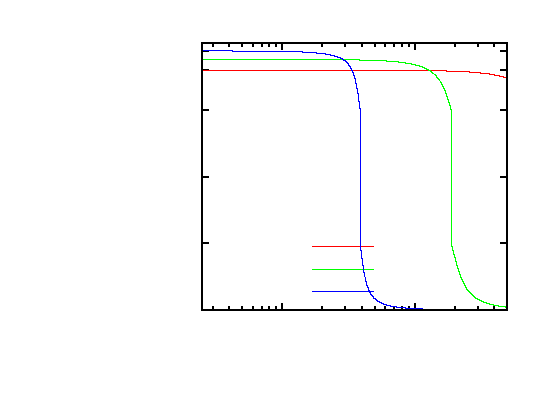
\includegraphics{c4_SHO}}%
    \gplfronttext
  \end{picture}%
\endgroup

  \label{fig:DeltaPhi}
  \caption{The difference between $\phib$ and $\phid$ with respect to frequency for bubbles of different radii.}
\end{figure}

When the bubble responds linearly to the driving pressure 
the relationship between the phase of the driving wave and the phase of the bubble can be determined analytically.
By linearising the acoustically-measured-Keller-Miksis equation (equation \eqnref{RKM} on page~\pageref{eqn:RKM})
so that $a(t) \rightarrow a_e + \epsilon$
we obtain
\begin{align}
 m \ddot \epsilon(t) + \lambda \dot \epsilon(t) + \omega_r^2 \epsilon(t) = A(t), \label{eqn:SHO}
\end{align}
where 
\begin{align}
  m &= a_e\lr{1+ \frac{4\mu}{a_enmc}}\\
  \lambda &= \frac{3\kappa}{nmc}\lr{p_0+\frac{2\sigma}{a}} + \frac{4\mu}{a_emn} - \frac{2\sigma}{a_e nmc}\\
  \omega_r^2 &= \frac{1}{a_enm}\lr{3\kappa \lr{p_0 +\frac{2\sigma}{a_e}} - \frac{2\sigma}{a_e}}\label{eqn:omegar}\\
\intertext{and}
  A &=- \frac{1}{nm}{p_i},
\end{align}
where $n$ is the equilibrium number density, $m$ is the mass per particle, $\mu$ is the dynamic viscosity $\sigma$ is the surface tension and 
 $\kappa= 1.4$ is the adiabatic polytropic index.
% \begin{align}
%   \lambda &= \lrsquare{\frac{4\mu}{nm a_e} + \frac{3 \kappa}{nm c} \lr{p_0+\frac{2\sigma{a_e}} - \frac{2\sigma}{nmac}}}
%     \lrsquare{1 - \frac{4\mu}{nma_ec}}^{-1},
% \end{align}
% \begin{align}
%   \omega_r^2 = \lrsquare{\frac{1}{nm a_e }\lr{3\kappa\lr{p_o + \frac{2\sigma}{a_e}} - \frac{2\sigma}{a}  }} \lrsquare{1 - \frac{4\mu}{nma_ec}}^{-1}
% \end{align}
% and 
% \begin{align}
% A(t) = -\frac{p_i}{nm} \lrsquare{1 - \frac{4\mu}{nma_ec}}^{-1}.
% \end{align}
We suppose in this subsection that the incident pulse is a pure sinusoid, with  $p_i \propto \cos(\omega(t))$.

Equation \eqnref{SHO} is the equation for a damped simple harmonic oscillator with solution
\begin{align}
\epsilon \propto \cos(\omega t + \beta). \label{eqn:SHO_soln}
\end{align}
The angle $\beta$ is the desired phase difference between $\phib$ and $\phid$ and is equal to 
\begin{align}
\beta = \tan^{-1}\lr{\frac{\lambda \omega}{m \omega^2-\omega_r^2}}.
\end{align}
As examples, \Figref{Phases} plots $\beta$ as a function of phase for a \unit{100}\nano\metre, \unit{300}\nano\metre\  and \unit{1}\micro\metre-radius bubble.
The phase difference drops rapidly at resonance.
% The
% As an example, 
% the phase difference of a \unit{100}\nano\metre-radius adiabatic ($\kappa = 1$) bubble when pulsated at \unit{0.5}\mega\pascal\ in water
% is
% \begin{align}
% \beta_{\unit{100}\nano\metre} = \tan^{-1}\lr{\frac{\lambda \omega}{\omega^2-\omega_r^2}}.
% \end{align}




\subsection{Characterising the scatter in two wave imaging}\label{sec:comp:optimum}

The scattering cross section, the quotient  of the scattered power to the incident intensity,  was used in \chapref{measurement} %(page~\pageref{eqn:sigmaff})
as a measure for the effectiveness of a contrast agent.
%The scattering cross section is the  quotient of the scattered power to the incident intensity
%for an infinite plain wave.
%and 
%was introduced in \secref{measurement:scatteringxs} on page~\pageref{eqn:sigmaff} for an infinite plain wave.
%It is a direct and well understood measure of the effectiveness of a contrast agent.
%We would like to understand the effectiveness of a contrast agent to an imaging wave 
%when the bubble is also in the presence of a driving wave, 
%which is not intended to be imaged.
%
%The scattering cross section is defined only at a single incident frequency (plain wave).
%We would therefore like to extend the notion.
%
%The scattering cross section for an infinite plain wave introduced in \secref{measurement:scatteringxs} on page~\pageref{eqn:sigmaff}.
The definition is repeated here for convenience,
\begin{align}
  \sigma(\omega) = 4\pi r^2 \oint dt \frac{ p^2  a^2}{\incp^2},\tag{\ref{eqn:sigmaff}}
\end{align}
where, $p$ is the emitted pressure, $\incp$  the incident  pressure, and $a$ is the bubble radius.
The integral is carried out over the
time period where both incident and emitted waves are stable - the closed integral sign being an mnemonic of this.
The incident pressure wave is an infinite plain wave and is therefore not applicable to the short pulses that are used in diagnostic ultrasound.
%This occurs when both the imaging and emitted wave oscillate an integer number of times within the period.
%However, this can make the scattering cross section hard to evaluate, 
%for such a period may not exist, or else may be very long, and hence hard to find numerically.
%Furthermore, it is not applicable to the short pulses that are used in diagnostic ultrasound.

Equation \eqnref{sigmaff} may be generalised to pulses by simply integrating over the whole pulse.
This is represented by an  open integration sign,
\begin{align}
  \pulseXS = 4\pi r^2\frac{ \int p^2 a^2dt}{ \int \incp^2dt} \label{eqn:sigmaPulse}.
\end{align} 
In general the bubble continues to ring after the driving pressure has stopped.
%This was seen in \figref{BubbleResponse}; the bubbles continued to ring after \unit{0}\micro\second,
The two integrals in \eqnref{sigmaPulse} are therefore not  over equal time periods.


When two different transducers are used to generate the two waves, however,
equation \eqnref{sigmaPulse} is no longer appropriate,
for it does not incorporate the 
%In general only the high harmonics of from the driving  wave are not filtered out by the 
limited frequency response of the imaging transducer.
The emitted pressure in \eqnref{sigmaff} section should be Fourier filtered.
In this thesis we model the response of the transducer with a 
Gaussian-shaped filter with a standard deviation on 25\% of the central frequency, $\mu$.
That is the Fourier filter, $\F,$ on the emitted pressure, $p = p(r,t)$, is,
\eqa{
  \F\lrsquare{p} = \iFFT  \lrsquare{e^{\frac{-8\lr{\omega - \mu}^2}{\mu^2}} \FFT\lrsquare{ p}}
%  \frac{1}{2\pi} \int d\omega \exp{frac{-2\lr{x - \mu}^2}{\mu^2}+i\omega t} 
%\int^t dt^\prime \exp\lr{-i \omega t^prime} p(x,t^\prime)
%\FFT^{-1} \lrsquare{\exp{frac{-2\lr{x - \mu}^2}{\mu^2}} \FFT\lrsquare{p_i(x)}  },
}
%The appropriate scattering cross section is therefore
%\begin{align}
%  4\pi r^2\frac{ \int_{\textrm{whole pulse} } \F \lrsquare{\lr{ p(r, t) a(t)}^2}dt}{ \int_{\textrm{whole pulse} }p_i(r,t)^2dt}  \nonumber
%\end{align}
where $\FFT$ is the Fourier transform  and $\FFT^{-1}$ is its inverse.


% \begin{figure}
%   \centering
%   \subfloat[Incident Pressure]{
%     \label{fig:Filtered:ipressure}
%     \includegraphics{bubble_ch4_ipressure.1}}
%   \label{fig:FreqRatio}
%   \qquad
%   \subfloat[Bubble Response]{
%     \label{fig:Filtered:response}
%     \includegraphics{bubble_ch4_rad.0}}
%   \\
%   \centering
%   % \centering
%   \subfloat[Emitted Pressure (unfiltered)]{
%     \label{fig:Filtered:pressure}
%     \includegraphics{bubble_ch4_out_pressure.2}}
%   \qquad
%   \subfloat[Emitted Pressure (filtered)]{
%     \label{fig:Filtered:filtered_pressure}
%     \includegraphics{bubble_ch4_out_filtered_pressure.3}}
%    \caption{In \figref{Filtered:ipressure} the incident pressure to a \unit{2}\micro\meter\ bubble is plotted.
% It consists of a 20 cycle, \unit{2}\mega\hertz\ driving pulse, driven at \unit{0.125}\mega\pascal\,
% and a 4 cycle, \unit{20}\mega\hertz\ imaging pulse driven at  \unit{1}\mega\pascal.
% The response of the bubble is plotted  in \figref{Filtered:response} using the acoustically-measured-Keller-Miksis equation.
% The calculated far-field emitted pressure  wave is plotted in \figref{Filtered:pressure}
% and the filtered emitted pressure is plotted in in \figref{Filtered:filtered_pressure}.   }
%   \label{fig:Filtered}
% \end{figure}


\begin{figure}
  \centering
  \subfloat[Incident Pressure]{
    \label{fig:Filtered:ipressure}
    \includegraphics{c4_fp_ipressure.0}}
  \label{fig:FreqRatio}
  \qquad
  \subfloat[Bubble Response]{
    \label{fig:Filtered:response}
    \includegraphics{c4_fp_radius.0}}
  \\
  \centering
  % \centering
  \subfloat[Emitted Pressure (unfiltered)]{
    \label{fig:Filtered:pressure}
    \includegraphics{c4_fp_gen_pressure.0}}
  \qquad
  \subfloat[Emitted Pressure (filtered)]{
    \label{fig:Filtered:filtered_pressure}
    \includegraphics{c4_fp_gen_pressure_filtered.0}}
   \caption{In \subref{fig:Filtered:ipressure} the incident pressure to a \unit{2}\micro\meter\ bubble is plotted.
It consists of a 20 cycle, \unit{2}\mega\hertz\ driving pulse, driven at \unit{0.125}\mega\pascal\,
and a 3 cycle, \unit{20}\mega\hertz\ imaging pulse driven at  \unit{1}\mega\pascal.
The response of the bubble is plotted  in \subref{fig:Filtered:response}.
The calculated far-field emitted pressure   is plotted in \subref{fig:Filtered:pressure}
and the filtered emitted pressure is plotted in  \subref{fig:Filtered:filtered_pressure}.  
The pressures are evaluated \unit{20}\milli\metre\ from the bubble }
  \label{fig:Filtered}
\end{figure}

\begin{figure}
  \centering
  \subfloat[Total Pressure]{
    \label{fig:DeltaPEffect:normal}
    \includegraphics{c4_fp_gen_pressure_filtered.0}}
  \label{fig:DeltaPEffect:excess}
  \qquad
  \subfloat[Excess Pressure]{
    \label{}
    \includegraphics{c4_fp_gen_pressure_excess.0}}
   \caption{A comparison between the total  pressure received by the imaging transducer 
     and the excess pressure received.
%   The excess pressure is the difference in pressure emitted when the imaging pulse is and is not present.
 Figure \subref{fig:DeltaPEffect:normal} is repeated from \figref{Filtered:filtered_pressure} for convenience
%\Figref{DeltaPEffecta} shows the emitted pressure as a function
%of the phase of the driving wave for a \unit{2}\mega\hertz\ driving wave (40 cycles, at \unit{0.1}\mega\pascal)
%and a \unit{20}\mega\hertz\ imaging wave (3 cycles, at \unit{1}\mega\pascal.
%\Figref{DelaaPEffectb} show the excess in emitted pressure under the same conditions.
}
  \label{fig:DeltaPEffect}
\end{figure}



The effect of the filter on a highly non-linear response is shown in \figref{Filtered}.
The filtered pressure in \figref{Filtered:filtered_pressure} does not retain only the response to the imaging wave,
but also the high frequency component of the bubble collapse and rebound.


The `breakthrough' of the response of the bubble to the driving wave
causes a difficulty in interpretation.
%For when interpreting the pressure received by the imaging transducer,
%the breakthrough signal does not arrive back at the appropriate time.
The imaging transducer measures the location of the bubble from the 
time at which the imaging pulse returns.
The first possibility is that the breakthrough signal that arrives before 
and after the imaging pulse will be attributed to  different spatial locations.
%This is because imaging transducer is ignorant to the fact that the signal actually came from the 
%response to the driving wave.
The imaging transducer will then measure  {\em phantom bubbles} in the image.
Alternatively,
if we know a priori through experimental setup that we are imaging just one bubble,
then the signal that arrives prior to the bubble breaks temporal ordering;
the bubble scatters before the imaging pulse arrives.

To overcome this difficulty more information is required by the imaging transducer.
This can be achieved by subtracting the  response of the bubble when there is no imaging wave.
This gives the excess pressure generated in response to the imaging wave,
\eqa{
  \Delta p = \F\lrsquare{\pdrim} - \F\lrsquare{\pdr}, \label{eqn:Deltap}
}
where $\pdrim$ is the pressure emitted when both driving and imaging pulses are incident,
and $\pdr$ is the pressure emitted in response to just the driving pulse.
The effect of equation \eqnref{Deltap}  is shown in \figref{DeltaPEffect}.
Most notably we see that the ringing is eliminated prior to the arrival of the imaging wave.
This is a great improvement because it restores temporal ordering to the high-frequency images.
%the bubble does not scatter before the imaging pulse arrives.
The remaining ringing after the arrival of the imaging wave occurs  
because the imaging wave perturbs the phase-space trajectory of the bubble into a different orbit.
While it still may be misinterpreted as phantom bubbles, it is at least a genuine response to the imaging wave.

%If we were to persist with the scattering cross section,
%then it could be argued that the scatter from the phantom bubbles should not be included.
%The scattering cross section would then be 
%
%The scatter from such phantoms will not be measured as coming from a bubble
%and so should not be included in the definition of the scatter of the bubble
%
%be included in the definition
%The bubble
%When interpreting the ultrasound image, 
%the scatter {\em from the bubble} occurs at the time at which the imaging pulse is assumed to be incident upon the 
%bubble.  Therefore, only the scatter occurring over the duration of the imaging pulse will be interpreted as being from the bubble.
%Any high frequency sound that is generated by the driving wave at times not sampled by the bubble
%will not be interpreted as being from the bubble.
%The appropriate scattering cross section for a bubble imaged with the high-frequency transducer is therefore
%\begin{align}
%   4\pi r^2\int dt\frac{ \lr{\F \lrsquare{p}}^2 a^2 }{p^2}, \label{eqn:imagXS}
%\end{align}
%where the integral is only for the duration of the imaging pulse.
%We shall not use this definition of the scattering cross section, however, 
%and therefore do not give it a symbol.




It is helpful to summarise the excess pressure plot into a single number.
For this purpose the excess scattering cross section is defined to be
\begin{align}
   \excessI = 4\pi \frac{ \int dt\lr{ \lrsquare{\Delta p}}^2 a^2 }{\int dt p_i^2}. \label{eqn:excessI}
\end{align}
%The normalisation with respect to the incident intensity is carried out to make the measure dimensionless\todo{In the sense that pressure is spherical on top and plainer on bottom so that r's cancel.  Need to say this better...}.
$\excessI$ is the  measure that we wish to optimise.

%Of perhaps more interest, however,  is the 
%excess generated intensity that can be attributed to a bubble (and which does not get attributed to phantom bubbles).
%The summary measure that is used most in this thesis, is therefore,
%\begin{align}
%   \imagI = 4\pi r^2\int dt\frac{ \lr{\F \lrsquare{p}}^2 }{p^2}, \label{eqn:imagI}
%\end{align}
%where the integral is over the duration of the imaging pulse only.
%It is $\imagI$ that we seek to maximise.





%Finally, in addition to the total scattering cross section,
%we are also interested in the temporal distribution of the emitted sound.
%For this, simply the ratio of the emitted intensity to the to total incident intensity will be used,
%\begin{align}
%  I(t) = 4\pi r^2 \frac{ \F \lrsquare{\lr{ p(r, t) a(t)}^2}}{\int p_i(r,t)^2} dt\label{eqn:IImaging}.
%\end{align}


\subsubsection{Reducing the phase-space perturbation in the bubble's response}\label{sec:reducing_perturbation}

% \begin{figure}[t]
%  \centering
%  \subfloat[Response to low amplitude incident waves]{
%    \label{fig:Phase_Pert:linear}
%    \includegraphics{c4_phase_pert_linear.0}}
% %
%  \subfloat[]{
%    \label{fig:Phase_Pert:nonlinearIm}
%    \includegraphics{c4_phase_pert_nonlinearIm.0}}
% %
%  \subfloat[Response to higher amplitude incident waves]{
%    \label{fig:Phase_Pert:nonlinearImDr}
%    \includegraphics{c4_phase_pert_nonlinearImDr.0}}
%  %
%   \caption{
% Phase-space trajectories of the bubble response to pulses with and without the imaging wave.
% When the amplitude is small the phase imaging wave does not appreciably alter the trajectory 
% In \subref{fig:fig:Phase_Pert:linear} the driving wave is 
% %
% A 10 cycle, \unit{0.5}\mega\hertz\ driving wave driven at \unit{10}\kilo\pascal\ 
% is incident on a \unit{2}\micro\metre\ bubble.
% The imaging wave is of 4 cycles at \unit{20}\mega\hertz driven at \unit{100}\kilo\pascal.
%    }
%  \label{fig:Phase_Pert}
% \end{figure}


\begin{figure}[t]
 \centering
 \subfloat[3-cycle imaging wave]{
   \label{fig:Phase_Pert:linear_short}
   \includegraphics{c4_phase_pert_linear_short.0}}
%
 \subfloat[10-cycle imaging wave]{
   \label{fig:Phase_Pert:linear_long}
   \includegraphics{c4_phase_pert_linear_long.0}}
%\\
% \subfloat[3-cycle imaging wave (high pressure)]{
%   \label{fig:Phase_Pert:nonlinearImDr_short}
%   \includegraphics{c4_phase_pert_nonlinearImDr_short.0}}
%%
% \subfloat[10-cycle imaging wave (high pressure)]{
%   \label{fig:Phase_Pert:nonlinearImDr_long}
%   \includegraphics{c4_phase_pert_nonlinearImDr_long.0}}
%
%5% \subfloat[Response to higher amplitude incident waves]{
%%   \label{fig:Phase_Pert:nonlinearImDr}
%%   \includegraphics{c4_phase_pert_nonlinearImDr.0}}
 %
  \caption{
The phase-space trajectory of \unit{2}\micro\metre-diameter bubble to short and long imaging pulses.
The driving pressure is  \unit{75}\kilo\pascal and the imaging wave pressure is  \unit{100}\kilo\pascal.
%at two different pressures.
%%In all the sub-figures the driving wave frequency is \unit{0.5}\mega\hertz\
%%and the imaging wave frequency is \unit{20}\mega\hertz.
%In  \subref{fig:Phase_Pert:linear_short} %and \subref{fig:Phase_Pert:linear_long}
%the driving wave pressure is  \unit{75}\kilo\pascal\
%and the imaging wave pressure is \unit{100}\kilo\pascal.
%In  \subref{fig:Phase_Pert:nonlinearImDr_short} and \subref{fig:Phase_Pert:nonlinearImDr_long}
%the driving wave pressure is  \unit{300}\kilo\pascal\
%and the imaging wave pressure is \unit{2}\mega\pascal.
%%Phase-space trajectories of the bubble response to pulses with and without the imaging wave.
%%When the amplitude is small the phase imaging wave does not appreciably alter the trajectory 
%%In \subref{fig:fig:Phase_Pert:linear} the driving wave is 
%%
%%A 10 cycle, \unit{0.5}\mega\hertz\ driving wave driven at \unit{10}\kilo\pascal\ 
%%is incident on a \unit{2}\micro\metre\ bubble.
%%The imaging wave is of 4 cycles at \unit{20}\mega\hertz driven at \unit{100}\kilo\pascal.
   }
 \label{fig:Phase_Pert}
\end{figure}


%\begin{figure}[t]
% \centering
% 
%
% \subfloat[Response to higher amplitude incident waves]{
%   \label{fig:Phase_Pert:nonlinearImDr}
%   \includegraphics{c4_phase_pert_nonlinearImDr.0}}
 %
%  \caption{
%Response of bubble to high amplitude incident waves.
%
%Phase-space trajectories of the bubble response to pulses with and without the imaging wave.
%When the amplitude is small the phase imaging wave does not appreciably alter the trajectory 
%In \subref{fig:fig:Phase_Pert:nonlinear_ImDr} the driving wave is 
%
%A 10 cycle, \unit{0.5}\mega\hertz\ driving wave driven at \unit{10}\kilo\pascal\ 
%is incident on a \unit{2}\micro\metre\ bubble.
%The imaging wave is of 4 cycles at \unit{20}\mega\hertz driven at \unit{100}\kilo\pascal.
%   }
% \label{fig:Phase_Pert}
%\end{figure}


A perturbation to the bubble's phase-space trajectory 
manifests itself as a ringing signal when it is filtered by the imaging transducer.
This ringing obfuscates the location of the bubble and so 
it is worthwhile understanding how the perturbation can be reduced.


%At low incident pressures the response of the bubble is approximately linear
%A sinusoidal input will result with a sinusoidal response.
%and the response from the driving and imaging waves can be considered separately 
%and then superposed.
The perturbation induced by the imaging wave will be small 
when the imaging pulse expands and contracts the bubble equally.
This will be true if the imaging pulse contains many cycles and the response of the bubble to it is linear.

If the pulse is short, however, the tempered tails of the pulse do not average out (\figref{comp:pulses:imaging})
and the bubble's expansion will not equal its compression.
This is seen in \figref{Phase_Pert}.
In each plot the response of a \unit{2}\micro\metre\ diameter bubble is drawn:
first in response to the driving wave alone (in red);
and second the response to both the driving and imaging waves (in black).
For a 3-cycle imaging wave (\figref{Phase_Pert:linear_short} %and \subref{fig:Phase_Pert:nonlinearImDr_short}) 
it is seen that the two trajectories are quite different, even at this low incident pressure.
However, as expected, the longer  10-cycle pulse returns to the unperturbed trajectory 
(\figref{Phase_Pert:linear_long}).

%It is easier to expand a bubble rather than to compress it
%and the response to a sinusoidal pressure will have an extended (in duration as well as amplitude) expansion phase
%and a short and sudden collapse. (See \figref{Filtered:response}, for example).
%A non-linear imaging wave will not return the bubble to where it would have been 
%for the bubble spent too long expanding in the incident pressure than contracting.
%This is seen in \figref{Phase_Pert:nonlinearIm}.

%These expectations are are confirmed with by plotting 
%To see this, trajectories for a single cycle of the driving wave are plotted in \figref{Phase_Pert}.

%At much higher pressures where non-linearity becomes important,
%the trajectories start to diverge again (\figref{Phase_Pert:nonlinearImDr_long}).

Similarly, 
a difference between the expansion and contraction stages of the bubbles oscillation
is characteristic of a nonlinear response.
As can be seen in \figref{Filtered:response}, for example,
the expansion phase is greater both in duration and amplitude.
We  expect, therefore, that the perturbation in  the bubble's phase space trajectory  to be greater 
when a nonlinear response is in its  expansion phase - 
for it is here that the nonlinearity has the time and amplitude to express itself.
This phase dependence will be  confirmed in \secref{phase_amp}.


In summary,
the ringing of the bubble in the excess pressure image can be reduced quite effectively 
by  reducing the time averaged pressure of the imaging wave to zero.
This is most easily achieved by increasing the number of cycles of the imaging wave,
although this is undesirable as it compromises resolution.
Careful synthesis of the imaging pulse to balance compression and rarefaction of the imaging pulse is not in the scope of this thesis,
and so we keep the uneven 3-cycle wave.
Indeed,  experiments in this thesis use a commercial scanner for imaging,
and the imaging pulse is not under experimental control.




%irrespective of the  amplitudes of the incident waves.
%For longer pulses at low amplitude (\figref{Phase_Pert:linear_long}),
%the trajectory returns to the original after the imaging pulse has completed.
%At higher pressures (\figref{Phase_Pert:nonlinearImDr_long}) the trajectories start to depart again.

%In summary, longer imaging pulses perturbing the bubble's  trajectory to a lesser degree than short pulses,
%likewise for lower amplitude pulses.
%The reason for this is that longer imaging pulses do better at 



%even though t
%This is compared to the response when the imaging wave is present (in black).
%In \figref{Phase_Pert_linear:short_pulse} a 3 cycle imaging wave is used.
%As seen from \figref{comp:pulses:imaging} the time spent in compression and expansion is not equal,
%and the bubble's trajectory is disturbed.
%In  \figref{Phase_Pert_linear:long_pulse} a 10 cycle imaging wave is used
%and the perturbation is much reduced.
%This is because for a longer pulse the time spent in compression and expansion is more even.



%At higher pressures the bubble no longer responds linearly.
%It is easier to expand a bubble rather than to compress it
%and the response to a sinusoidal pressure will have an extended (in duration as well as amplitude) expansion phase
%and a short and sudden collapse. (See \figref{Filtered:response}, for example).
%A non-linear imaging wave will not return the bubble to where it would have been 
%for the bubble spent too long expanding in the incident pressure than contracting.
%This is seen in \figref{Phase_Pert:nonlinearIm}.


%As a representative of this group we plot in \figref{Phase_Pert:nonlinearImDr} the change in orbit for the bubble response of \figref{Filtered:response}.


%The response of the bubble to the incident driving and imaging waves is not linear;
%no superposition principle holds.
%In general the bubble's response cannot be attributed to either of the waves alone.

%The response of the bubble to the incident pressure is not linear.
%It is easier to expand a bubble rather than to compress it.
%A sinusoidal incident pressure will not result in a sinusoidal response,
%but will have an extended (in duration as well as amplitude) expansion phase
%and a short and sudden collapse.


%In general the bubble's response cannot be attributed to either of the waves alone.
%However, when the duration of the imaging wave is short in comparison to the period of the driving wave,
%it may be hoped that its influence on the pulsation induced by the driving wave is minimal.
%This chapter investigates the degree to which this is true.

%In \secref{comp:optimum} we found that a perturbation to the bubble's phase-space trajectory 
%manifests itself in a ringing signal when it is filtered by the imaging transducer.
%This ringing obfuscates the location of the bubble and so attempting to reduce the perturbation is worthwhile.
%The phase-space perturbation evidently depends on the degree of non-linearity,
%but also on the  time available for the non-linearity to manifest itself.
%To keep the ringing in the excess pressure to a minimum,
%the imaging pulse should be kept as short as possible,  with respect to the timescale defined by the driving frequency.

%In \figref{} a near-linear driving wave and non-linear imaging wave is incident upon a \unit{2}\micro\metre\ bubble.
%In \figref{} a higher pressure driving wave is used.

%\subsubsection{Change of orbit}


% \begin{figure}
%   \centering
%   \subfloat[$n=1$]{
%     \label{fig:FreqRatioContour1}
%     \includegraphics{FreqRatioContour1.0}}
%   \qquad
%   \subfloat[$n=3$]{
%     \label{fig:FreqRatioContour3}
%     \includegraphics{FreqRatioContour3.0}}
%   \label{fig:FreqRatio}
%   \\
%   \centering
%   % \centering
%   \subfloat[$\phi_d = \pi/2$]{
%     \label{fig:FreqRatioMinRange}
%     \includegraphics{FreqRatioContourMinError.0}}
%   \qquad
%   \subfloat[$\phi_d = \pi$]{
%     \label{fig:FreqRatioMaxRange}
%     \includegraphics{FreqRatioContourMaxError.0}}
%    \caption{
%      Plots of $p$ evaluated from \eqnref{FreqRatio}.
%      In \subref{fig:FreqRatioContour1} and \subref{fig:FreqRatioContour3} contour plots for the ratio $\frac{ \omega_i }{\omega_d}$ and phases of the driving wave
%      for $n=1$ and $n=3$.
%      In  \subref{fig:FreqRatioMaxRange} and \subref{fig:FreqRatioMinRange}, $p$ evaluated or various values of $n$ at the phases $\phi_d = \pi$ and $\phi_d = \pi/2$.
%    }
%   \label{fig:FreqRatio}
% \end{figure}

% %In reality the imaging pulse has a non-negligible width with respect to the driving wave.
% %Therefore, the imaging pulse will sample a range of phases of the driving pulse.
% %The range of phases, however, is not of primary interest,
% %rather it is the range of pressures sampled by the imaging wave.
% Since the driving pressure is fluctuating
% an imaging wave of any finite duration will sample a range of driving pressures.
% This range will be greatest when the driving wave pressure is changing most rapidly,
% when $\phi_d = 0, \pi/2 ,\ldots$, etc.



% %which occurs at a time, $t$, such that the pressure passes through its equilibrium value.
% %These points shall be taken to be at the phases $m\pi$, such that $m$ is an integer.
% If the imaging wave oscillate for $n/2$ cycles at a frequency $\omega_i$ either side of the stated driving phase,
% then the percentage pressures sampled, $s$, by the imaging wave is,
% \newcommand{\intv}[2]{\text{interval}\left[ #1, #2 \right]}
% \begin{align}
%   s &=\intv{ f\lr{\omega_d \lr{t-\frac{n}{2\omega_i}}}}{ f\lr{\omega_d\lr{t+\frac{n}{2\omega}}}  } \times 100\%\label{eqn:FreqRatio}\\
%   \text{where}\quad
%   f(x)  &= \tfrac{1}{2} \lr{\sin(x)+1}
% \end{align}
% and the notation $\intv{\cdot}{\cdot}$ indicates the interval spanned in the range of the two arguments.


% %The first factor on the right of \eqnref{FreqRatio} gives the dependence of the range on the phase of the 
% %driving wave.
% %The ratio, $\frac{ \omega_i }{\omega_d}$, in the second factor is of most interest, however.
% %This ratio gives the imaging frequency, as a multiple of the driving frequency,
% %required for the range of radii to be below some set percentage.

% % \begin{minipage}{1.2in}

% % \end{minipage}%

% \Figref{FreqRatio} plots  $s$  as a function of the ratio $\frac{ \omega_i }{\omega_d}$
% and the phase $\phi$ for various values of $n$.
% In \Figref{FreqRatioContour1} %the contours in the value of $p$ are illustrated as a function of the ratio
% %$\frac{ \omega_i }{\omega_d}$ and the phase of the driving wave for when $n=1$. 
% When  $n=1$, for the range to be less than $5\%$ a ratio of $10$ between the frequencies of the two 
% waves is required.
% In practise, ringing in the transducer will always prevent just a single oscillation being produced,
% with $3$ or $4$ cycles usually the minimum excitation.
% The contour plot case for $n=3$ is illustrated in \figref{FreqRatioContour3}.
% In this case, a ratio of $30$  between the frequencies of the two 
% waves is required to keep the range below $5\%$.
% \Figref{FreqRatioMaxRange} plots the ratio $\frac{ \omega_i }{\omega_d}$  against $p$
% at a phase in the driving wave where the range is maximum.


% To understand how the percentage overlap effects the degree to which the orbit changes we 
% compare the orbit they driving cycle after the imaging wave was involved with what it would have been 
% had the imaging wave not been present.
% The two signals are cross correlated and the ratio of this with the autocorrelation of the signal without the imaging
% wave is taken.

% This is plotted for the driving frequency of \unit{0.5}\mega\hertz taken at 0.01, 0.1 and 0.5 \mega\pascal,
% for the response of a 2 \micro\metre\ bubble.


% Comments...


\section{How the parameters influence each other}\label{sec:comp:examples}

In the introduction we chose \numparam\ parameters to investigate:
the frequencies and amplitudes of the incident driving and imaging waves,
$\frd$, $\fri$, $\Ad$ and $\Ai$;
the time lag between the two waves, $\phidi$;
and the radius of the bubble, $a$.
%These  parameters are chosen to be a minimal set characterising the bubble response to two wave imaging.
%Of these variables the amplitudes and the time lag can generally be altered within a given experiment,
%and are therefore give the finest degree of control.
%The frequencies are set in hardware and 
%the distribution of  bubble radii is hard to determine never-mind control for short lived bubbles.

%a property of the transducer and are less easy to change,
%while the radii of the bubble is distributed 
%In this section we priorities efforts of this section to these parameters.
%The frequencies o

The time lag between the imaging and driving waves is the most interesting, 
as it controls the part of the bubble's phase trajectory that get sampled by the imaging wave.
This section investigates how the other parameters change the scattering as a function of $\phidi$.


\subsection{The scatter as a function of driving phase} \label{sec:excess_phase}


\begin{figure}
 \centering
% \subfloat[$n=1$]{
%   \label{fig:phase_vs_phase:a}
%  % GNUPLOT: LaTeX picture with Postscript
\begingroup
  \makeatletter
  \providecommand\color[2][]{%
    \GenericError{(gnuplot) \space\space\space\@spaces}{%
      Package color not loaded in conjunction with
      terminal option `colourtext'%
    }{See the gnuplot documentation for explanation.%
    }{Either use 'blacktext' in gnuplot or load the package
      color.sty in LaTeX.}%
    \renewcommand\color[2][]{}%
  }%
  \providecommand\includegraphics[2][]{%
    \GenericError{(gnuplot) \space\space\space\@spaces}{%
      Package graphicx or graphics not loaded%
    }{See the gnuplot documentation for explanation.%
    }{The gnuplot epslatex terminal needs graphicx.sty or graphics.sty.}%
    \renewcommand\includegraphics[2][]{}%
  }%
  \providecommand\rotatebox[2]{#2}%
  \@ifundefined{ifGPcolor}{%
    \newif\ifGPcolor
    \GPcolorfalse
  }{}%
  \@ifundefined{ifGPblacktext}{%
    \newif\ifGPblacktext
    \GPblacktexttrue
  }{}%
  % define a \g@addto@macro without @ in the name:
  \let\gplgaddtomacro\g@addto@macro
  % define empty templates for all commands taking text:
  \gdef\gplbacktext{}%
  \gdef\gplfronttext{}%
  \makeatother
  \ifGPblacktext
    % no textcolor at all
    \def\colorrgb#1{}%
    \def\colorgray#1{}%
  \else
    % gray or color?
    \ifGPcolor
      \def\colorrgb#1{\color[rgb]{#1}}%
      \def\colorgray#1{\color[gray]{#1}}%
      \expandafter\def\csname LTw\endcsname{\color{white}}%
      \expandafter\def\csname LTb\endcsname{\color{black}}%
      \expandafter\def\csname LTa\endcsname{\color{black}}%
      \expandafter\def\csname LT0\endcsname{\color[rgb]{1,0,0}}%
      \expandafter\def\csname LT1\endcsname{\color[rgb]{0,1,0}}%
      \expandafter\def\csname LT2\endcsname{\color[rgb]{0,0,1}}%
      \expandafter\def\csname LT3\endcsname{\color[rgb]{1,0,1}}%
      \expandafter\def\csname LT4\endcsname{\color[rgb]{0,1,1}}%
      \expandafter\def\csname LT5\endcsname{\color[rgb]{1,1,0}}%
      \expandafter\def\csname LT6\endcsname{\color[rgb]{0,0,0}}%
      \expandafter\def\csname LT7\endcsname{\color[rgb]{1,0.3,0}}%
      \expandafter\def\csname LT8\endcsname{\color[rgb]{0.5,0.5,0.5}}%
    \else
      % gray
      \def\colorrgb#1{\color{black}}%
      \def\colorgray#1{\color[gray]{#1}}%
      \expandafter\def\csname LTw\endcsname{\color{white}}%
      \expandafter\def\csname LTb\endcsname{\color{black}}%
      \expandafter\def\csname LTa\endcsname{\color{black}}%
      \expandafter\def\csname LT0\endcsname{\color{black}}%
      \expandafter\def\csname LT1\endcsname{\color{black}}%
      \expandafter\def\csname LT2\endcsname{\color{black}}%
      \expandafter\def\csname LT3\endcsname{\color{black}}%
      \expandafter\def\csname LT4\endcsname{\color{black}}%
      \expandafter\def\csname LT5\endcsname{\color{black}}%
      \expandafter\def\csname LT6\endcsname{\color{black}}%
      \expandafter\def\csname LT7\endcsname{\color{black}}%
      \expandafter\def\csname LT8\endcsname{\color{black}}%
    \fi
  \fi
  \setlength{\unitlength}{0.0500bp}%
  \begin{picture}(7200.00,5040.00)%
    \gplgaddtomacro\gplbacktext{%
      \csname LTb\endcsname%
      \put(588,1008){\makebox(0,0)[r]{\strut{}0}}%
      \put(588,1283){\makebox(0,0)[r]{\strut{}$2\pi$}}%
      \put(588,1558){\makebox(0,0)[r]{\strut{}$4\pi$}}%
      \put(588,1833){\makebox(0,0)[r]{\strut{}$6\pi$}}%
      \put(588,2108){\makebox(0,0)[r]{\strut{}$8\pi$}}%
      \put(588,2383){\makebox(0,0)[r]{\strut{}$10\pi$}}%
      \put(588,2657){\makebox(0,0)[r]{\strut{}$12\pi$}}%
      \put(588,2932){\makebox(0,0)[r]{\strut{}$14\pi$}}%
      \put(588,3207){\makebox(0,0)[r]{\strut{}$16\pi$}}%
      \put(588,3482){\makebox(0,0)[r]{\strut{}$18\pi$}}%
      \put(588,3757){\makebox(0,0)[r]{\strut{}$20\pi$}}%
      \put(720,788){\makebox(0,0){\strut{}$10^{0}$}}%
      \put(1080,788){\makebox(0,0){\strut{}$10^{1}$}}%
      \put(1440,788){\makebox(0,0){\strut{}$10^{2}$}}%
      \put(1800,788){\makebox(0,0){\strut{}$10^{3}$}}%
      \put(-50,2520){\rotatebox{90}{\makebox(0,0){\strut{}sampled driving phase, $\phi_{d0}$}}}%
      \put(1260,458){\makebox(0,0){\strut{}driving phase, $\phi_d$}}%
    }%
    \gplgaddtomacro\gplfronttext{%
    }%
    \gplgaddtomacro\gplbacktext{%
    }%
    \gplgaddtomacro\gplfronttext{%
      \csname LTb\endcsname%
      \put(1801,641){\makebox(0,0){\strut{}0}}%
      \put(2259,641){\makebox(0,0){\strut{}$2\pi$}}%
      \put(2717,641){\makebox(0,0){\strut{}$4\pi$}}%
      \put(3175,641){\makebox(0,0){\strut{}$6\pi$}}%
      \put(3633,641){\makebox(0,0){\strut{}$8\pi$}}%
      \put(4091,641){\makebox(0,0){\strut{}$10\pi$}}%
      \put(4549,641){\makebox(0,0){\strut{}$12\pi$}}%
      \put(5007,641){\makebox(0,0){\strut{}$14\pi$}}%
      \put(5465,641){\makebox(0,0){\strut{}$16\pi$}}%
      \put(5923,641){\makebox(0,0){\strut{}$18\pi$}}%
      \put(6381,641){\makebox(0,0){\strut{}$20\pi$}}%
      \put(4320,311){\makebox(0,0){\strut{}driving phase, $\phi_d$}}%
    }%
    \gplbacktext
    \put(0,0){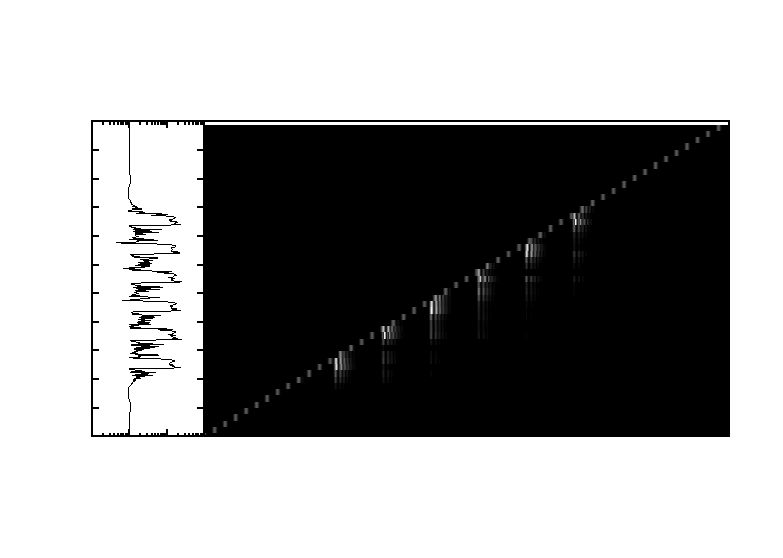
\includegraphics{c4_phase_vs_phase_1}}%
    \gplfronttext
  \end{picture}%
\endgroup
}
% \subfloat[$n=1$]{
%   \label{fig:phase_vs_phase:b}
  % GNUPLOT: LaTeX picture with Postscript
\begingroup
  \makeatletter
  \providecommand\color[2][]{%
    \GenericError{(gnuplot) \space\space\space\@spaces}{%
      Package color not loaded in conjunction with
      terminal option `colourtext'%
    }{See the gnuplot documentation for explanation.%
    }{Either use 'blacktext' in gnuplot or load the package
      color.sty in LaTeX.}%
    \renewcommand\color[2][]{}%
  }%
  \providecommand\includegraphics[2][]{%
    \GenericError{(gnuplot) \space\space\space\@spaces}{%
      Package graphicx or graphics not loaded%
    }{See the gnuplot documentation for explanation.%
    }{The gnuplot epslatex terminal needs graphicx.sty or graphics.sty.}%
    \renewcommand\includegraphics[2][]{}%
  }%
  \providecommand\rotatebox[2]{#2}%
  \@ifundefined{ifGPcolor}{%
    \newif\ifGPcolor
    \GPcolorfalse
  }{}%
  \@ifundefined{ifGPblacktext}{%
    \newif\ifGPblacktext
    \GPblacktexttrue
  }{}%
  % define a \g@addto@macro without @ in the name:
  \let\gplgaddtomacro\g@addto@macro
  % define empty templates for all commands taking text:
  \gdef\gplbacktext{}%
  \gdef\gplfronttext{}%
  \makeatother
  \ifGPblacktext
    % no textcolor at all
    \def\colorrgb#1{}%
    \def\colorgray#1{}%
  \else
    % gray or color?
    \ifGPcolor
      \def\colorrgb#1{\color[rgb]{#1}}%
      \def\colorgray#1{\color[gray]{#1}}%
      \expandafter\def\csname LTw\endcsname{\color{white}}%
      \expandafter\def\csname LTb\endcsname{\color{black}}%
      \expandafter\def\csname LTa\endcsname{\color{black}}%
      \expandafter\def\csname LT0\endcsname{\color[rgb]{1,0,0}}%
      \expandafter\def\csname LT1\endcsname{\color[rgb]{0,1,0}}%
      \expandafter\def\csname LT2\endcsname{\color[rgb]{0,0,1}}%
      \expandafter\def\csname LT3\endcsname{\color[rgb]{1,0,1}}%
      \expandafter\def\csname LT4\endcsname{\color[rgb]{0,1,1}}%
      \expandafter\def\csname LT5\endcsname{\color[rgb]{1,1,0}}%
      \expandafter\def\csname LT6\endcsname{\color[rgb]{0,0,0}}%
      \expandafter\def\csname LT7\endcsname{\color[rgb]{1,0.3,0}}%
      \expandafter\def\csname LT8\endcsname{\color[rgb]{0.5,0.5,0.5}}%
    \else
      % gray
      \def\colorrgb#1{\color{black}}%
      \def\colorgray#1{\color[gray]{#1}}%
      \expandafter\def\csname LTw\endcsname{\color{white}}%
      \expandafter\def\csname LTb\endcsname{\color{black}}%
      \expandafter\def\csname LTa\endcsname{\color{black}}%
      \expandafter\def\csname LT0\endcsname{\color{black}}%
      \expandafter\def\csname LT1\endcsname{\color{black}}%
      \expandafter\def\csname LT2\endcsname{\color{black}}%
      \expandafter\def\csname LT3\endcsname{\color{black}}%
      \expandafter\def\csname LT4\endcsname{\color{black}}%
      \expandafter\def\csname LT5\endcsname{\color{black}}%
      \expandafter\def\csname LT6\endcsname{\color{black}}%
      \expandafter\def\csname LT7\endcsname{\color{black}}%
      \expandafter\def\csname LT8\endcsname{\color{black}}%
    \fi
  \fi
  \setlength{\unitlength}{0.0500bp}%
  \begin{picture}(7200.00,6300.00)%
    \gplgaddtomacro\gplbacktext{%
      \csname LTb\endcsname%
      \put(588,1008){\makebox(0,0)[r]{\strut{}0}}%
      \put(588,1336){\makebox(0,0)[r]{\strut{}$2\pi$}}%
      \put(588,1663){\makebox(0,0)[r]{\strut{}$4\pi$}}%
      \put(588,1991){\makebox(0,0)[r]{\strut{}$6\pi$}}%
      \put(588,2318){\makebox(0,0)[r]{\strut{}$8\pi$}}%
      \put(588,2646){\makebox(0,0)[r]{\strut{}$10\pi$}}%
      \put(588,2974){\makebox(0,0)[r]{\strut{}$12\pi$}}%
      \put(588,3301){\makebox(0,0)[r]{\strut{}$14\pi$}}%
      \put(588,3629){\makebox(0,0)[r]{\strut{}$16\pi$}}%
      \put(588,3956){\makebox(0,0)[r]{\strut{}$18\pi$}}%
      \put(588,4284){\makebox(0,0)[r]{\strut{}$20\pi$}}%
      \put(720,788){\makebox(0,0){\strut{}$10^{0}$}}%
      \put(1260,788){\makebox(0,0){\strut{}$10^{1}$}}%
      \put(1800,788){\makebox(0,0){\strut{}$10^{2}$}}%
      \put(-50,2646){\rotatebox{90}{\makebox(0,0){\strut{}sampled driving phase, $\phi_{d0}$}}}%
      \put(1260,293){\makebox(0,0){\strut{}$\sigma_{ex}$}}%
    }%
    \gplgaddtomacro\gplfronttext{%
    }%
    \gplgaddtomacro\gplbacktext{%
      \csname LTb\endcsname%
      \put(1668,4392){\makebox(0,0)[r]{\strut{}-0.1}}%
      \put(1668,4536){\makebox(0,0)[r]{\strut{} 0}}%
      \put(1668,4680){\makebox(0,0)[r]{\strut{} 0.1}}%
      \put(1800,5008){\makebox(0,0){\strut{}0}}%
      \put(2808,5008){\makebox(0,0){\strut{}4$\pi$}}%
      \put(3816,5008){\makebox(0,0){\strut{}8$\pi$}}%
      \put(4824,5008){\makebox(0,0){\strut{}12$\pi$}}%
      \put(5832,5008){\makebox(0,0){\strut{}16$\pi$}}%
      \put(6840,5008){\makebox(0,0){\strut{}20$\pi$}}%
      \put(1030,4536){\rotatebox{90}{\makebox(0,0){\strut{}MPa}}}%
      \put(4320,4218){\makebox(0,0){\strut{}}}%
    }%
    \gplgaddtomacro\gplfronttext{%
    }%
    \gplgaddtomacro\gplbacktext{%
    }%
    \gplgaddtomacro\gplfronttext{%
      \csname LTb\endcsname%
      \put(1801,641){\makebox(0,0){\strut{}0}}%
      \put(2305,641){\makebox(0,0){\strut{}$2\pi$}}%
      \put(2809,641){\makebox(0,0){\strut{}$4\pi$}}%
      \put(3313,641){\makebox(0,0){\strut{}$6\pi$}}%
      \put(3817,641){\makebox(0,0){\strut{}$8\pi$}}%
      \put(4320,641){\makebox(0,0){\strut{}$10\pi$}}%
      \put(4823,641){\makebox(0,0){\strut{}$12\pi$}}%
      \put(5327,641){\makebox(0,0){\strut{}$14\pi$}}%
      \put(5831,641){\makebox(0,0){\strut{}$16\pi$}}%
      \put(6335,641){\makebox(0,0){\strut{}$18\pi$}}%
      \put(6839,641){\makebox(0,0){\strut{}$20\pi$}}%
      \put(4320,311){\makebox(0,0){\strut{}driving phase, $\phi_d$}}%
    }%
    \gplbacktext
    \put(0,0){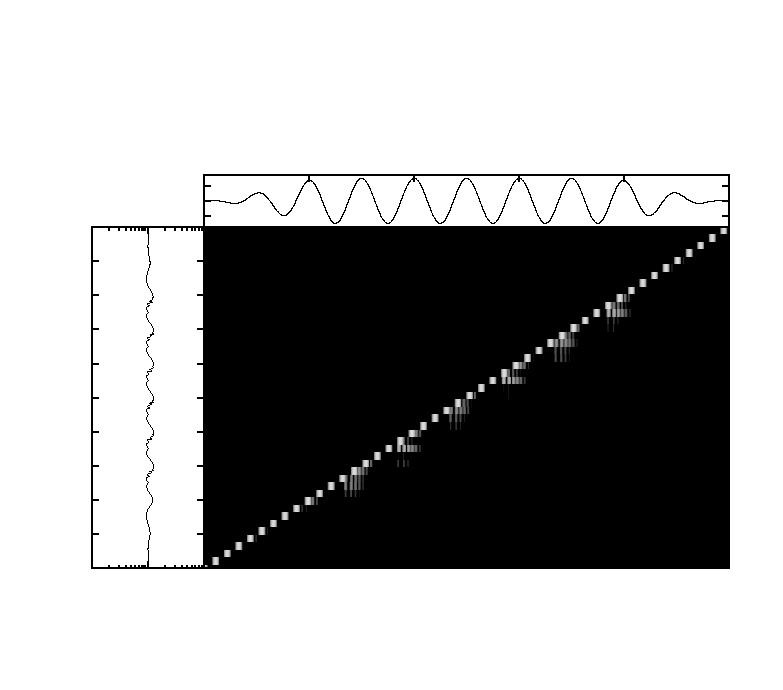
\includegraphics{c4_phase_vs_phase_low_2}}%
    \gplfronttext
  \end{picture}%
\endgroup

%}
   % 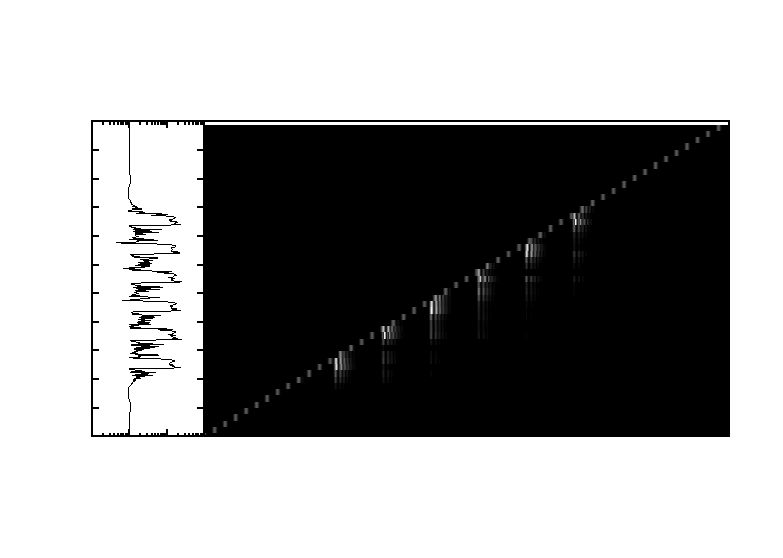
\includegraphics{c4_phase_vs_phase_1.t}}
  \caption{
The excess pressure and the excess scattering cross section as a function of $\phidi$ and $\phid$
for a \unit{2}\micro\metre-diameter bubble pulsated with a driving wave of \unit{150}\kilo\pascal.
Also shown is the excess scattering cross section, $\excessI$, and the driving pulse used.
  }
 \label{fig:excess_vs_phase}
\end{figure}


 \begin{figure}[p]
   \centering 
  % \subfloat[$n=1$]{
  %   \label{fig:excess_vs_phase:mapping:a}
  %   \includegraphics{c4_excess_mapping.0}}
   \subfloat[]{
     \label{fig:excess_vs_phase:mapping:map}
     \includegraphics{c4_excess_mapping_a.0}}
   \subfloat[]{
     \label{fig:excess_vs_phase:mapping:bubble}
     \includegraphics{c4_excess_mapping_c.0}}\\
   \subfloat[]{
     \label{fig:excess_vs_phase:mapping:driving}
     \includegraphics{c4_excess_mapping_b.0}}
   \subfloat[phase-space trajectory]{
     \label{fig:excess_vs_phase:mapping:phasor}
     \includegraphics{c4_excess_mapping_d.1}}
   \label{fig:FreqRatio}
    \caption{
      The relationship between $\phid$ and $\phib$ from \figref{excess_vs_phase} is plotted in \subref{fig:excess_vs_phase:mapping:map} 
      for a $2\pi$ segment.
      This maps the excess scattering cross section $\excessI$ from being a function of the driving phase in 
      \subref{fig:excess_vs_phase:mapping:driving} to a function of the bubble's phase in 
      \subref{fig:excess_vs_phase:mapping:bubble}.
      Figure \subref{fig:excess_vs_phase:mapping:phasor} plots the phase-space trajectory of the 
      bubble in response to the driving pulse (without the imaging wave)
      The arrow indicates the location of the trajectory where the bubble's phase is $17\pi$.
   }
   \label{fig:excess_vs_phase:mapping}
 \end{figure}
We begin by considering the dependence of the excess pressure, a function of the driving phase, $\phid$,
on the dependence of the sampled driving phase, $\phidi$.
%from \eqnref{Deltap},
%on the time-lag between the two pulses.
%
%
%To do this the excess pressure, $\excessI$ from \eqnref{Deltap},
%is evaluated as  as a function $\phidi$, the driving phase sampled by the imaging wave,
%and the driving phase, $\phid$.
%, $\excessI$ from \eqnref\eqnref{Deltap} 
A grayscale plot of $\excessI(\phid,\phidi)$ is hard to visually interpret, however,
due zero being mid-gray.
For this reason, and also due to the familiarity of B-mode images in ultrasound,
we plot the Hilbert transform of the excess pressure.
This is done in  \figref{excess_vs_phase} for a \unit{2}\micro\metre-diameter 
bubble pulsated with a \unit{150}\kilo\pascal, 
\unit{0.5}\mega\hertz\ driving wave, 
and a \unit{500}\kilo\pascal, \unit{20}\mega\hertz\ imaging wave.
In \figref{excess_vs_phase} we also plot the excess scattering cross section from equation \eqnref{excessI} (on the left),
and the driving pulse used (on the top).




\Figref{excess_vs_phase} shows that the excess scattering cross section oscillates with the same periodicity
as the driving pressure
and that the scatter is high when driving pressure is high.
If the bubble were responding linearly
then the phase with respect to the driving wave would be expected to be $-0.18$ (\figref{DeltaPhi}).
A high pressure would therefore correspond to a contracted bubble.
%In this, case, however, the response from the bubble is far from linear.

In this case, however, the response of the bubble to the driving pulse is far from linear.
\figref{excess_vs_phase:mapping:phasor} shows the phase-space trajectory of the bubble for the range $8\pi\le\phid<10\pi$.
The mapping between the bubble's phase and the driving phase is plotted in \subref{fig:excess_vs_phase:mapping:map}.
We find that for the $2\pi$ change in the driving wave the bubble's phase actually changes by $6\pi$;
the harmonics are already dominating.
Nevertheless, it still remains true that the excess scattering cross section is  greatest when the bubble is small.
This is seen by mapping  $\excessI(\phid) \rightarrow \excessI(\phib)$,
which is carried out in by going from Figure~\subref{fig:excess_vs_phase:mapping:driving} to \subref{fig:excess_vs_phase:mapping:bubble}
via \subref{fig:excess_vs_phase:mapping:map}.
The scattering is maximal at the bubble phases $-17\pi - 6m\pi$, for integer $m$, which corresponds to the bubble being small.
The arrow in \figref{excess_vs_phase:mapping:phasor} indicates the phase-space position when $\phib = -17\pi$.

The increase in the scattering when the bubble is shrunk has a simple interpretation.
From \figref{DeltaPhi} we see that a \unit{300}\nano\metre bubble is resonant at about \unit{20}\mega\hertz.
A \unit{2}\micro\metre-diameter bubble is larger than this.
However, by shrinking it you are transiently creating a bubble that is closer to its resonance - and therefore increasing its scattering cross section.


% In \figref{excess_vs_phase:mapping}, the map between the driving and bubble phase, 
% \subref{fig:excess_vs_phase:mapping:a}, is used to 
% plot the excess scattering cross section as a function of 
% the driving phase,  \subref{fig:excess_vs_phase:mapping:b},
% and the bubble's phase, \subref{fig:excess_vs_phase:mapping:c}.
% We see,
% therefore, 
% that the driving excess intensity is more symmetric when considered a function of the .... phase.
% The intensity is high when the bubble's phase is ...
% and low when the bubbles phase is ...
% Therefore the intensity 

%If the total scattering rather than the excess scattering cross section had been plotted,
%then \Figref{excess_vs_phase:total_mapping} becomes.
%It is seen that the phase dependence is swamped by the response to the driving wave.


% \begin {figure}
%   \begin{center}
%     % GNUPLOT: LaTeX picture with Postscript
\begingroup
  \makeatletter
  \providecommand\color[2][]{%
    \GenericError{(gnuplot) \space\space\space\@spaces}{%
      Package color not loaded in conjunction with
      terminal option `colourtext'%
    }{See the gnuplot documentation for explanation.%
    }{Either use 'blacktext' in gnuplot or load the package
      color.sty in LaTeX.}%
    \renewcommand\color[2][]{}%
  }%
  \providecommand\includegraphics[2][]{%
    \GenericError{(gnuplot) \space\space\space\@spaces}{%
      Package graphicx or graphics not loaded%
    }{See the gnuplot documentation for explanation.%
    }{The gnuplot epslatex terminal needs graphicx.sty or graphics.sty.}%
    \renewcommand\includegraphics[2][]{}%
  }%
  \providecommand\rotatebox[2]{#2}%
  \@ifundefined{ifGPcolor}{%
    \newif\ifGPcolor
    \GPcolorfalse
  }{}%
  \@ifundefined{ifGPblacktext}{%
    \newif\ifGPblacktext
    \GPblacktexttrue
  }{}%
  % define a \g@addto@macro without @ in the name:
  \let\gplgaddtomacro\g@addto@macro
  % define empty templates for all commands taking text:
  \gdef\gplbacktext{}%
  \gdef\gplfronttext{}%
  \makeatother
  \ifGPblacktext
    % no textcolor at all
    \def\colorrgb#1{}%
    \def\colorgray#1{}%
  \else
    % gray or color?
    \ifGPcolor
      \def\colorrgb#1{\color[rgb]{#1}}%
      \def\colorgray#1{\color[gray]{#1}}%
      \expandafter\def\csname LTw\endcsname{\color{white}}%
      \expandafter\def\csname LTb\endcsname{\color{black}}%
      \expandafter\def\csname LTa\endcsname{\color{black}}%
      \expandafter\def\csname LT0\endcsname{\color[rgb]{1,0,0}}%
      \expandafter\def\csname LT1\endcsname{\color[rgb]{0,1,0}}%
      \expandafter\def\csname LT2\endcsname{\color[rgb]{0,0,1}}%
      \expandafter\def\csname LT3\endcsname{\color[rgb]{1,0,1}}%
      \expandafter\def\csname LT4\endcsname{\color[rgb]{0,1,1}}%
      \expandafter\def\csname LT5\endcsname{\color[rgb]{1,1,0}}%
      \expandafter\def\csname LT6\endcsname{\color[rgb]{0,0,0}}%
      \expandafter\def\csname LT7\endcsname{\color[rgb]{1,0.3,0}}%
      \expandafter\def\csname LT8\endcsname{\color[rgb]{0.5,0.5,0.5}}%
    \else
      % gray
      \def\colorrgb#1{\color{black}}%
      \def\colorgray#1{\color[gray]{#1}}%
      \expandafter\def\csname LTw\endcsname{\color{white}}%
      \expandafter\def\csname LTb\endcsname{\color{black}}%
      \expandafter\def\csname LTa\endcsname{\color{black}}%
      \expandafter\def\csname LT0\endcsname{\color{black}}%
      \expandafter\def\csname LT1\endcsname{\color{black}}%
      \expandafter\def\csname LT2\endcsname{\color{black}}%
      \expandafter\def\csname LT3\endcsname{\color{black}}%
      \expandafter\def\csname LT4\endcsname{\color{black}}%
      \expandafter\def\csname LT5\endcsname{\color{black}}%
      \expandafter\def\csname LT6\endcsname{\color{black}}%
      \expandafter\def\csname LT7\endcsname{\color{black}}%
      \expandafter\def\csname LT8\endcsname{\color{black}}%
    \fi
  \fi
  \setlength{\unitlength}{0.0500bp}%
  \begin{picture}(7200.00,5040.00)%
    \gplgaddtomacro\gplbacktext{%
      \csname LTb\endcsname%
      \put(588,1008){\makebox(0,0)[r]{\strut{}0}}%
      \put(588,1283){\makebox(0,0)[r]{\strut{}$2\pi$}}%
      \put(588,1558){\makebox(0,0)[r]{\strut{}$4\pi$}}%
      \put(588,1833){\makebox(0,0)[r]{\strut{}$6\pi$}}%
      \put(588,2108){\makebox(0,0)[r]{\strut{}$8\pi$}}%
      \put(588,2383){\makebox(0,0)[r]{\strut{}$10\pi$}}%
      \put(588,2657){\makebox(0,0)[r]{\strut{}$12\pi$}}%
      \put(588,2932){\makebox(0,0)[r]{\strut{}$14\pi$}}%
      \put(588,3207){\makebox(0,0)[r]{\strut{}$16\pi$}}%
      \put(588,3482){\makebox(0,0)[r]{\strut{}$18\pi$}}%
      \put(588,3757){\makebox(0,0)[r]{\strut{}$20\pi$}}%
      \put(720,788){\makebox(0,0){\strut{}$10^{0}$}}%
      \put(1080,788){\makebox(0,0){\strut{}$10^{1}$}}%
      \put(1440,788){\makebox(0,0){\strut{}$10^{2}$}}%
      \put(1800,788){\makebox(0,0){\strut{}$10^{3}$}}%
      \put(-50,2520){\rotatebox{90}{\makebox(0,0){\strut{}sampled driving phase, $\phi_{d0}$}}}%
      \put(1260,458){\makebox(0,0){\strut{}driving phase, $\phi_d$}}%
    }%
    \gplgaddtomacro\gplfronttext{%
    }%
    \gplgaddtomacro\gplbacktext{%
    }%
    \gplgaddtomacro\gplfronttext{%
      \csname LTb\endcsname%
      \put(1801,641){\makebox(0,0){\strut{}0}}%
      \put(2259,641){\makebox(0,0){\strut{}$2\pi$}}%
      \put(2717,641){\makebox(0,0){\strut{}$4\pi$}}%
      \put(3175,641){\makebox(0,0){\strut{}$6\pi$}}%
      \put(3633,641){\makebox(0,0){\strut{}$8\pi$}}%
      \put(4091,641){\makebox(0,0){\strut{}$10\pi$}}%
      \put(4549,641){\makebox(0,0){\strut{}$12\pi$}}%
      \put(5007,641){\makebox(0,0){\strut{}$14\pi$}}%
      \put(5465,641){\makebox(0,0){\strut{}$16\pi$}}%
      \put(5923,641){\makebox(0,0){\strut{}$18\pi$}}%
      \put(6381,641){\makebox(0,0){\strut{}$20\pi$}}%
      \put(4320,311){\makebox(0,0){\strut{}driving phase, $\phi_d$}}%
    }%
    \gplbacktext
    \put(0,0){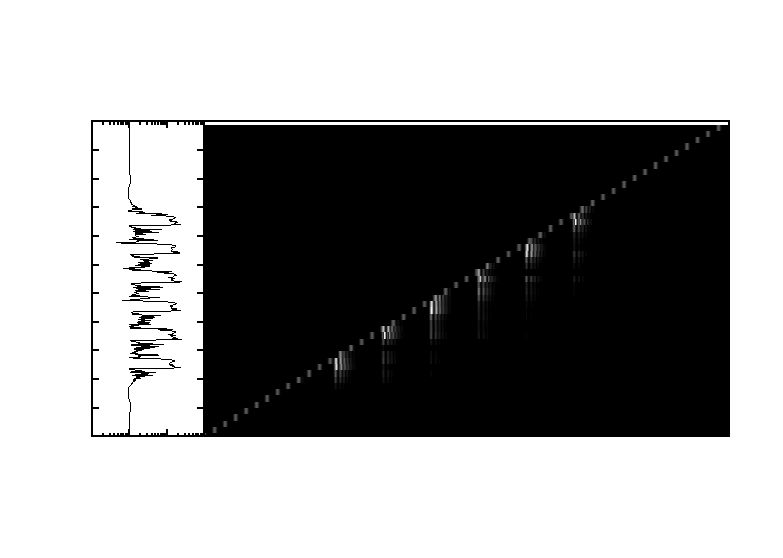
\includegraphics{c4_phase_vs_phase_1}}%
    \gplfronttext
  \end{picture}%
\endgroup

%   \end{center}
% \end {figure}


% \begin{figure}
%  \centering
%  \subfloat[$n=1$]{
%    \label{fig:phase_vs_phase:a}
%   % GNUPLOT: LaTeX picture with Postscript
\begingroup
  \makeatletter
  \providecommand\color[2][]{%
    \GenericError{(gnuplot) \space\space\space\@spaces}{%
      Package color not loaded in conjunction with
      terminal option `colourtext'%
    }{See the gnuplot documentation for explanation.%
    }{Either use 'blacktext' in gnuplot or load the package
      color.sty in LaTeX.}%
    \renewcommand\color[2][]{}%
  }%
  \providecommand\includegraphics[2][]{%
    \GenericError{(gnuplot) \space\space\space\@spaces}{%
      Package graphicx or graphics not loaded%
    }{See the gnuplot documentation for explanation.%
    }{The gnuplot epslatex terminal needs graphicx.sty or graphics.sty.}%
    \renewcommand\includegraphics[2][]{}%
  }%
  \providecommand\rotatebox[2]{#2}%
  \@ifundefined{ifGPcolor}{%
    \newif\ifGPcolor
    \GPcolorfalse
  }{}%
  \@ifundefined{ifGPblacktext}{%
    \newif\ifGPblacktext
    \GPblacktexttrue
  }{}%
  % define a \g@addto@macro without @ in the name:
  \let\gplgaddtomacro\g@addto@macro
  % define empty templates for all commands taking text:
  \gdef\gplbacktext{}%
  \gdef\gplfronttext{}%
  \makeatother
  \ifGPblacktext
    % no textcolor at all
    \def\colorrgb#1{}%
    \def\colorgray#1{}%
  \else
    % gray or color?
    \ifGPcolor
      \def\colorrgb#1{\color[rgb]{#1}}%
      \def\colorgray#1{\color[gray]{#1}}%
      \expandafter\def\csname LTw\endcsname{\color{white}}%
      \expandafter\def\csname LTb\endcsname{\color{black}}%
      \expandafter\def\csname LTa\endcsname{\color{black}}%
      \expandafter\def\csname LT0\endcsname{\color[rgb]{1,0,0}}%
      \expandafter\def\csname LT1\endcsname{\color[rgb]{0,1,0}}%
      \expandafter\def\csname LT2\endcsname{\color[rgb]{0,0,1}}%
      \expandafter\def\csname LT3\endcsname{\color[rgb]{1,0,1}}%
      \expandafter\def\csname LT4\endcsname{\color[rgb]{0,1,1}}%
      \expandafter\def\csname LT5\endcsname{\color[rgb]{1,1,0}}%
      \expandafter\def\csname LT6\endcsname{\color[rgb]{0,0,0}}%
      \expandafter\def\csname LT7\endcsname{\color[rgb]{1,0.3,0}}%
      \expandafter\def\csname LT8\endcsname{\color[rgb]{0.5,0.5,0.5}}%
    \else
      % gray
      \def\colorrgb#1{\color{black}}%
      \def\colorgray#1{\color[gray]{#1}}%
      \expandafter\def\csname LTw\endcsname{\color{white}}%
      \expandafter\def\csname LTb\endcsname{\color{black}}%
      \expandafter\def\csname LTa\endcsname{\color{black}}%
      \expandafter\def\csname LT0\endcsname{\color{black}}%
      \expandafter\def\csname LT1\endcsname{\color{black}}%
      \expandafter\def\csname LT2\endcsname{\color{black}}%
      \expandafter\def\csname LT3\endcsname{\color{black}}%
      \expandafter\def\csname LT4\endcsname{\color{black}}%
      \expandafter\def\csname LT5\endcsname{\color{black}}%
      \expandafter\def\csname LT6\endcsname{\color{black}}%
      \expandafter\def\csname LT7\endcsname{\color{black}}%
      \expandafter\def\csname LT8\endcsname{\color{black}}%
    \fi
  \fi
  \setlength{\unitlength}{0.0500bp}%
  \begin{picture}(7200.00,5040.00)%
    \gplgaddtomacro\gplbacktext{%
      \csname LTb\endcsname%
      \put(588,1008){\makebox(0,0)[r]{\strut{}0}}%
      \put(588,1283){\makebox(0,0)[r]{\strut{}$2\pi$}}%
      \put(588,1558){\makebox(0,0)[r]{\strut{}$4\pi$}}%
      \put(588,1833){\makebox(0,0)[r]{\strut{}$6\pi$}}%
      \put(588,2108){\makebox(0,0)[r]{\strut{}$8\pi$}}%
      \put(588,2383){\makebox(0,0)[r]{\strut{}$10\pi$}}%
      \put(588,2657){\makebox(0,0)[r]{\strut{}$12\pi$}}%
      \put(588,2932){\makebox(0,0)[r]{\strut{}$14\pi$}}%
      \put(588,3207){\makebox(0,0)[r]{\strut{}$16\pi$}}%
      \put(588,3482){\makebox(0,0)[r]{\strut{}$18\pi$}}%
      \put(588,3757){\makebox(0,0)[r]{\strut{}$20\pi$}}%
      \put(720,788){\makebox(0,0){\strut{}$10^{0}$}}%
      \put(1080,788){\makebox(0,0){\strut{}$10^{1}$}}%
      \put(1440,788){\makebox(0,0){\strut{}$10^{2}$}}%
      \put(1800,788){\makebox(0,0){\strut{}$10^{3}$}}%
      \put(-50,2520){\rotatebox{90}{\makebox(0,0){\strut{}sampled driving phase, $\phi_{d0}$}}}%
      \put(1260,458){\makebox(0,0){\strut{}driving phase, $\phi_d$}}%
    }%
    \gplgaddtomacro\gplfronttext{%
    }%
    \gplgaddtomacro\gplbacktext{%
    }%
    \gplgaddtomacro\gplfronttext{%
      \csname LTb\endcsname%
      \put(1801,641){\makebox(0,0){\strut{}0}}%
      \put(2259,641){\makebox(0,0){\strut{}$2\pi$}}%
      \put(2717,641){\makebox(0,0){\strut{}$4\pi$}}%
      \put(3175,641){\makebox(0,0){\strut{}$6\pi$}}%
      \put(3633,641){\makebox(0,0){\strut{}$8\pi$}}%
      \put(4091,641){\makebox(0,0){\strut{}$10\pi$}}%
      \put(4549,641){\makebox(0,0){\strut{}$12\pi$}}%
      \put(5007,641){\makebox(0,0){\strut{}$14\pi$}}%
      \put(5465,641){\makebox(0,0){\strut{}$16\pi$}}%
      \put(5923,641){\makebox(0,0){\strut{}$18\pi$}}%
      \put(6381,641){\makebox(0,0){\strut{}$20\pi$}}%
      \put(4320,311){\makebox(0,0){\strut{}driving phase, $\phi_d$}}%
    }%
    \gplbacktext
    \put(0,0){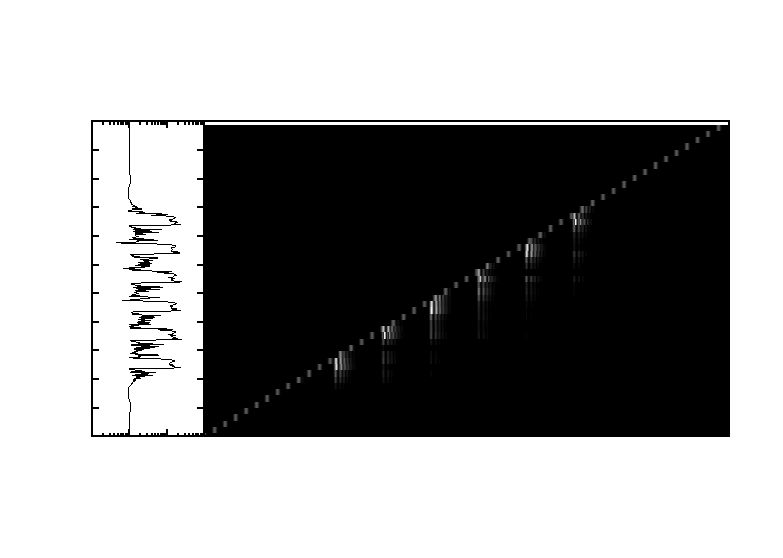
\includegraphics{c4_phase_vs_phase_1}}%
    \gplfronttext
  \end{picture}%
\endgroup
}
%  \subfloat[$n=1$]{
%    \label{fig:phase_vs_phase:b}
%   % GNUPLOT: LaTeX picture with Postscript
\begingroup
  \makeatletter
  \providecommand\color[2][]{%
    \GenericError{(gnuplot) \space\space\space\@spaces}{%
      Package color not loaded in conjunction with
      terminal option `colourtext'%
    }{See the gnuplot documentation for explanation.%
    }{Either use 'blacktext' in gnuplot or load the package
      color.sty in LaTeX.}%
    \renewcommand\color[2][]{}%
  }%
  \providecommand\includegraphics[2][]{%
    \GenericError{(gnuplot) \space\space\space\@spaces}{%
      Package graphicx or graphics not loaded%
    }{See the gnuplot documentation for explanation.%
    }{The gnuplot epslatex terminal needs graphicx.sty or graphics.sty.}%
    \renewcommand\includegraphics[2][]{}%
  }%
  \providecommand\rotatebox[2]{#2}%
  \@ifundefined{ifGPcolor}{%
    \newif\ifGPcolor
    \GPcolorfalse
  }{}%
  \@ifundefined{ifGPblacktext}{%
    \newif\ifGPblacktext
    \GPblacktexttrue
  }{}%
  % define a \g@addto@macro without @ in the name:
  \let\gplgaddtomacro\g@addto@macro
  % define empty templates for all commands taking text:
  \gdef\gplbacktext{}%
  \gdef\gplfronttext{}%
  \makeatother
  \ifGPblacktext
    % no textcolor at all
    \def\colorrgb#1{}%
    \def\colorgray#1{}%
  \else
    % gray or color?
    \ifGPcolor
      \def\colorrgb#1{\color[rgb]{#1}}%
      \def\colorgray#1{\color[gray]{#1}}%
      \expandafter\def\csname LTw\endcsname{\color{white}}%
      \expandafter\def\csname LTb\endcsname{\color{black}}%
      \expandafter\def\csname LTa\endcsname{\color{black}}%
      \expandafter\def\csname LT0\endcsname{\color[rgb]{1,0,0}}%
      \expandafter\def\csname LT1\endcsname{\color[rgb]{0,1,0}}%
      \expandafter\def\csname LT2\endcsname{\color[rgb]{0,0,1}}%
      \expandafter\def\csname LT3\endcsname{\color[rgb]{1,0,1}}%
      \expandafter\def\csname LT4\endcsname{\color[rgb]{0,1,1}}%
      \expandafter\def\csname LT5\endcsname{\color[rgb]{1,1,0}}%
      \expandafter\def\csname LT6\endcsname{\color[rgb]{0,0,0}}%
      \expandafter\def\csname LT7\endcsname{\color[rgb]{1,0.3,0}}%
      \expandafter\def\csname LT8\endcsname{\color[rgb]{0.5,0.5,0.5}}%
    \else
      % gray
      \def\colorrgb#1{\color{black}}%
      \def\colorgray#1{\color[gray]{#1}}%
      \expandafter\def\csname LTw\endcsname{\color{white}}%
      \expandafter\def\csname LTb\endcsname{\color{black}}%
      \expandafter\def\csname LTa\endcsname{\color{black}}%
      \expandafter\def\csname LT0\endcsname{\color{black}}%
      \expandafter\def\csname LT1\endcsname{\color{black}}%
      \expandafter\def\csname LT2\endcsname{\color{black}}%
      \expandafter\def\csname LT3\endcsname{\color{black}}%
      \expandafter\def\csname LT4\endcsname{\color{black}}%
      \expandafter\def\csname LT5\endcsname{\color{black}}%
      \expandafter\def\csname LT6\endcsname{\color{black}}%
      \expandafter\def\csname LT7\endcsname{\color{black}}%
      \expandafter\def\csname LT8\endcsname{\color{black}}%
    \fi
  \fi
  \setlength{\unitlength}{0.0500bp}%
  \begin{picture}(7200.00,5040.00)%
    \gplgaddtomacro\gplbacktext{%
      \csname LTb\endcsname%
      \put(588,1008){\makebox(0,0)[r]{\strut{}0}}%
      \put(588,1283){\makebox(0,0)[r]{\strut{}$2\pi$}}%
      \put(588,1558){\makebox(0,0)[r]{\strut{}$4\pi$}}%
      \put(588,1833){\makebox(0,0)[r]{\strut{}$6\pi$}}%
      \put(588,2108){\makebox(0,0)[r]{\strut{}$8\pi$}}%
      \put(588,2383){\makebox(0,0)[r]{\strut{}$10\pi$}}%
      \put(588,2657){\makebox(0,0)[r]{\strut{}$12\pi$}}%
      \put(588,2932){\makebox(0,0)[r]{\strut{}$14\pi$}}%
      \put(588,3207){\makebox(0,0)[r]{\strut{}$16\pi$}}%
      \put(588,3482){\makebox(0,0)[r]{\strut{}$18\pi$}}%
      \put(588,3757){\makebox(0,0)[r]{\strut{}$20\pi$}}%
      \put(720,788){\makebox(0,0){\strut{}$10^{0}$}}%
      \put(1080,788){\makebox(0,0){\strut{}$10^{1}$}}%
      \put(1440,788){\makebox(0,0){\strut{}$10^{2}$}}%
      \put(1800,788){\makebox(0,0){\strut{}$10^{3}$}}%
      \put(-50,2520){\rotatebox{90}{\makebox(0,0){\strut{}sampled driving phase, $\phi_{d0}$}}}%
      \put(1260,293){\makebox(0,0){\strut{}$\sigma_{ex}$}}%
    }%
    \gplgaddtomacro\gplfronttext{%
    }%
    \gplgaddtomacro\gplbacktext{%
    }%
    \gplgaddtomacro\gplfronttext{%
      \csname LTb\endcsname%
      \put(1801,641){\makebox(0,0){\strut{}0}}%
      \put(2259,641){\makebox(0,0){\strut{}$2\pi$}}%
      \put(2717,641){\makebox(0,0){\strut{}$4\pi$}}%
      \put(3175,641){\makebox(0,0){\strut{}$6\pi$}}%
      \put(3633,641){\makebox(0,0){\strut{}$8\pi$}}%
      \put(4091,641){\makebox(0,0){\strut{}$10\pi$}}%
      \put(4549,641){\makebox(0,0){\strut{}$12\pi$}}%
      \put(5007,641){\makebox(0,0){\strut{}$14\pi$}}%
      \put(5465,641){\makebox(0,0){\strut{}$16\pi$}}%
      \put(5923,641){\makebox(0,0){\strut{}$18\pi$}}%
      \put(6381,641){\makebox(0,0){\strut{}$20\pi$}}%
      \put(4320,147){\makebox(0,0){\strut{}$\sigma_{ex}$}}%
    }%
    \gplbacktext
    \put(0,0){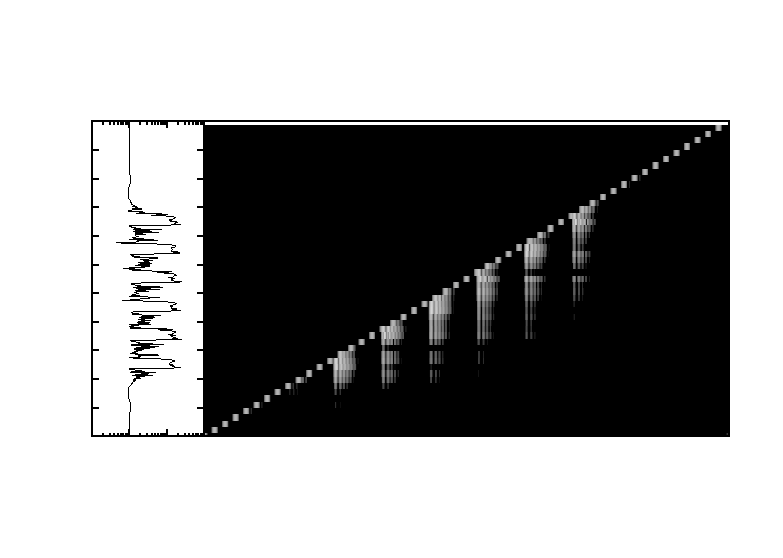
\includegraphics{c4_phase_vs_phase_2}}%
    \gplfronttext
  \end{picture}%
\endgroup
}
%    % 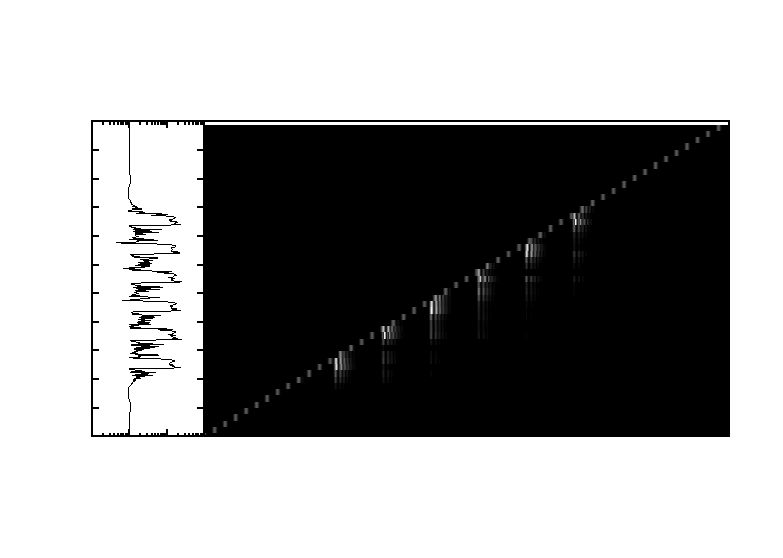
\includegraphics{c4_phase_vs_phase_1.t}}
%   \caption{
%   }
%  \label{fig:phase_vs_phase}
% \end{figure}

% \begin{figure}
%  \centering
%  \subfloat[$n=1$]{
%    \label{fig:phase_vs_phase_low:a}
%   % GNUPLOT: LaTeX picture with Postscript
\begingroup
  \makeatletter
  \providecommand\color[2][]{%
    \GenericError{(gnuplot) \space\space\space\@spaces}{%
      Package color not loaded in conjunction with
      terminal option `colourtext'%
    }{See the gnuplot documentation for explanation.%
    }{Either use 'blacktext' in gnuplot or load the package
      color.sty in LaTeX.}%
    \renewcommand\color[2][]{}%
  }%
  \providecommand\includegraphics[2][]{%
    \GenericError{(gnuplot) \space\space\space\@spaces}{%
      Package graphicx or graphics not loaded%
    }{See the gnuplot documentation for explanation.%
    }{The gnuplot epslatex terminal needs graphicx.sty or graphics.sty.}%
    \renewcommand\includegraphics[2][]{}%
  }%
  \providecommand\rotatebox[2]{#2}%
  \@ifundefined{ifGPcolor}{%
    \newif\ifGPcolor
    \GPcolorfalse
  }{}%
  \@ifundefined{ifGPblacktext}{%
    \newif\ifGPblacktext
    \GPblacktexttrue
  }{}%
  % define a \g@addto@macro without @ in the name:
  \let\gplgaddtomacro\g@addto@macro
  % define empty templates for all commands taking text:
  \gdef\gplbacktext{}%
  \gdef\gplfronttext{}%
  \makeatother
  \ifGPblacktext
    % no textcolor at all
    \def\colorrgb#1{}%
    \def\colorgray#1{}%
  \else
    % gray or color?
    \ifGPcolor
      \def\colorrgb#1{\color[rgb]{#1}}%
      \def\colorgray#1{\color[gray]{#1}}%
      \expandafter\def\csname LTw\endcsname{\color{white}}%
      \expandafter\def\csname LTb\endcsname{\color{black}}%
      \expandafter\def\csname LTa\endcsname{\color{black}}%
      \expandafter\def\csname LT0\endcsname{\color[rgb]{1,0,0}}%
      \expandafter\def\csname LT1\endcsname{\color[rgb]{0,1,0}}%
      \expandafter\def\csname LT2\endcsname{\color[rgb]{0,0,1}}%
      \expandafter\def\csname LT3\endcsname{\color[rgb]{1,0,1}}%
      \expandafter\def\csname LT4\endcsname{\color[rgb]{0,1,1}}%
      \expandafter\def\csname LT5\endcsname{\color[rgb]{1,1,0}}%
      \expandafter\def\csname LT6\endcsname{\color[rgb]{0,0,0}}%
      \expandafter\def\csname LT7\endcsname{\color[rgb]{1,0.3,0}}%
      \expandafter\def\csname LT8\endcsname{\color[rgb]{0.5,0.5,0.5}}%
    \else
      % gray
      \def\colorrgb#1{\color{black}}%
      \def\colorgray#1{\color[gray]{#1}}%
      \expandafter\def\csname LTw\endcsname{\color{white}}%
      \expandafter\def\csname LTb\endcsname{\color{black}}%
      \expandafter\def\csname LTa\endcsname{\color{black}}%
      \expandafter\def\csname LT0\endcsname{\color{black}}%
      \expandafter\def\csname LT1\endcsname{\color{black}}%
      \expandafter\def\csname LT2\endcsname{\color{black}}%
      \expandafter\def\csname LT3\endcsname{\color{black}}%
      \expandafter\def\csname LT4\endcsname{\color{black}}%
      \expandafter\def\csname LT5\endcsname{\color{black}}%
      \expandafter\def\csname LT6\endcsname{\color{black}}%
      \expandafter\def\csname LT7\endcsname{\color{black}}%
      \expandafter\def\csname LT8\endcsname{\color{black}}%
    \fi
  \fi
  \setlength{\unitlength}{0.0500bp}%
  \begin{picture}(7200.00,5040.00)%
    \gplgaddtomacro\gplbacktext{%
      \csname LTb\endcsname%
      \put(588,1008){\makebox(0,0)[r]{\strut{}0}}%
      \put(588,1283){\makebox(0,0)[r]{\strut{}$2\pi$}}%
      \put(588,1558){\makebox(0,0)[r]{\strut{}$4\pi$}}%
      \put(588,1833){\makebox(0,0)[r]{\strut{}$6\pi$}}%
      \put(588,2108){\makebox(0,0)[r]{\strut{}$8\pi$}}%
      \put(588,2383){\makebox(0,0)[r]{\strut{}$10\pi$}}%
      \put(588,2657){\makebox(0,0)[r]{\strut{}$12\pi$}}%
      \put(588,2932){\makebox(0,0)[r]{\strut{}$14\pi$}}%
      \put(588,3207){\makebox(0,0)[r]{\strut{}$16\pi$}}%
      \put(588,3482){\makebox(0,0)[r]{\strut{}$18\pi$}}%
      \put(588,3757){\makebox(0,0)[r]{\strut{}$20\pi$}}%
      \put(720,788){\makebox(0,0){\strut{}$10^{0}$}}%
      \put(1260,788){\makebox(0,0){\strut{}$10^{1}$}}%
      \put(1800,788){\makebox(0,0){\strut{}$10^{2}$}}%
      \put(-50,2520){\rotatebox{90}{\makebox(0,0){\strut{}sampled driving phase, $\phi_{d0}$}}}%
      \put(1260,293){\makebox(0,0){\strut{}$\sigma_{ex}$}}%
    }%
    \gplgaddtomacro\gplfronttext{%
    }%
    \gplgaddtomacro\gplbacktext{%
    }%
    \gplgaddtomacro\gplfronttext{%
      \csname LTb\endcsname%
      \put(1801,641){\makebox(0,0){\strut{}0}}%
      \put(2259,641){\makebox(0,0){\strut{}$2\pi$}}%
      \put(2717,641){\makebox(0,0){\strut{}$4\pi$}}%
      \put(3175,641){\makebox(0,0){\strut{}$6\pi$}}%
      \put(3633,641){\makebox(0,0){\strut{}$8\pi$}}%
      \put(4091,641){\makebox(0,0){\strut{}$10\pi$}}%
      \put(4549,641){\makebox(0,0){\strut{}$12\pi$}}%
      \put(5007,641){\makebox(0,0){\strut{}$14\pi$}}%
      \put(5465,641){\makebox(0,0){\strut{}$16\pi$}}%
      \put(5923,641){\makebox(0,0){\strut{}$18\pi$}}%
      \put(6381,641){\makebox(0,0){\strut{}$20\pi$}}%
      \put(4320,147){\makebox(0,0){\strut{}$\sigma_{ex}$}}%
    }%
    \gplbacktext
    \put(0,0){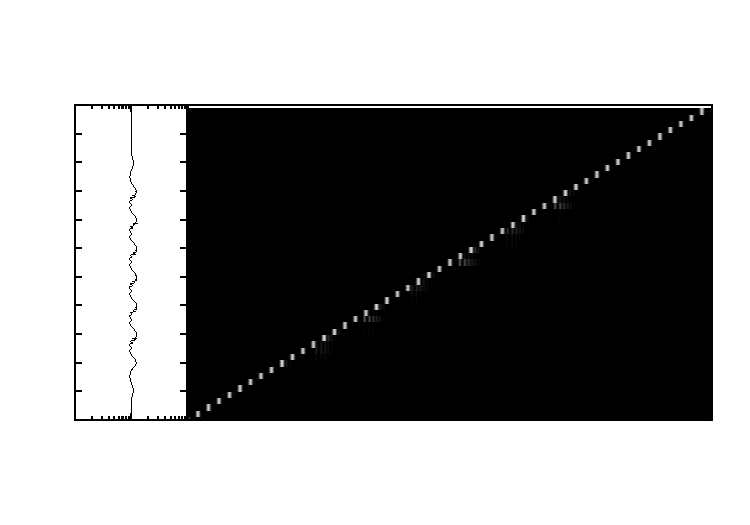
\includegraphics{c4_phase_vs_phase_low_1}}%
    \gplfronttext
  \end{picture}%
\endgroup
}
%  \subfloat[$n=1$]{
%    \label{fig:phase_vs_phase_low:b}
%   % GNUPLOT: LaTeX picture with Postscript
\begingroup
  \makeatletter
  \providecommand\color[2][]{%
    \GenericError{(gnuplot) \space\space\space\@spaces}{%
      Package color not loaded in conjunction with
      terminal option `colourtext'%
    }{See the gnuplot documentation for explanation.%
    }{Either use 'blacktext' in gnuplot or load the package
      color.sty in LaTeX.}%
    \renewcommand\color[2][]{}%
  }%
  \providecommand\includegraphics[2][]{%
    \GenericError{(gnuplot) \space\space\space\@spaces}{%
      Package graphicx or graphics not loaded%
    }{See the gnuplot documentation for explanation.%
    }{The gnuplot epslatex terminal needs graphicx.sty or graphics.sty.}%
    \renewcommand\includegraphics[2][]{}%
  }%
  \providecommand\rotatebox[2]{#2}%
  \@ifundefined{ifGPcolor}{%
    \newif\ifGPcolor
    \GPcolorfalse
  }{}%
  \@ifundefined{ifGPblacktext}{%
    \newif\ifGPblacktext
    \GPblacktexttrue
  }{}%
  % define a \g@addto@macro without @ in the name:
  \let\gplgaddtomacro\g@addto@macro
  % define empty templates for all commands taking text:
  \gdef\gplbacktext{}%
  \gdef\gplfronttext{}%
  \makeatother
  \ifGPblacktext
    % no textcolor at all
    \def\colorrgb#1{}%
    \def\colorgray#1{}%
  \else
    % gray or color?
    \ifGPcolor
      \def\colorrgb#1{\color[rgb]{#1}}%
      \def\colorgray#1{\color[gray]{#1}}%
      \expandafter\def\csname LTw\endcsname{\color{white}}%
      \expandafter\def\csname LTb\endcsname{\color{black}}%
      \expandafter\def\csname LTa\endcsname{\color{black}}%
      \expandafter\def\csname LT0\endcsname{\color[rgb]{1,0,0}}%
      \expandafter\def\csname LT1\endcsname{\color[rgb]{0,1,0}}%
      \expandafter\def\csname LT2\endcsname{\color[rgb]{0,0,1}}%
      \expandafter\def\csname LT3\endcsname{\color[rgb]{1,0,1}}%
      \expandafter\def\csname LT4\endcsname{\color[rgb]{0,1,1}}%
      \expandafter\def\csname LT5\endcsname{\color[rgb]{1,1,0}}%
      \expandafter\def\csname LT6\endcsname{\color[rgb]{0,0,0}}%
      \expandafter\def\csname LT7\endcsname{\color[rgb]{1,0.3,0}}%
      \expandafter\def\csname LT8\endcsname{\color[rgb]{0.5,0.5,0.5}}%
    \else
      % gray
      \def\colorrgb#1{\color{black}}%
      \def\colorgray#1{\color[gray]{#1}}%
      \expandafter\def\csname LTw\endcsname{\color{white}}%
      \expandafter\def\csname LTb\endcsname{\color{black}}%
      \expandafter\def\csname LTa\endcsname{\color{black}}%
      \expandafter\def\csname LT0\endcsname{\color{black}}%
      \expandafter\def\csname LT1\endcsname{\color{black}}%
      \expandafter\def\csname LT2\endcsname{\color{black}}%
      \expandafter\def\csname LT3\endcsname{\color{black}}%
      \expandafter\def\csname LT4\endcsname{\color{black}}%
      \expandafter\def\csname LT5\endcsname{\color{black}}%
      \expandafter\def\csname LT6\endcsname{\color{black}}%
      \expandafter\def\csname LT7\endcsname{\color{black}}%
      \expandafter\def\csname LT8\endcsname{\color{black}}%
    \fi
  \fi
  \setlength{\unitlength}{0.0500bp}%
  \begin{picture}(7200.00,6300.00)%
    \gplgaddtomacro\gplbacktext{%
      \csname LTb\endcsname%
      \put(588,1008){\makebox(0,0)[r]{\strut{}0}}%
      \put(588,1336){\makebox(0,0)[r]{\strut{}$2\pi$}}%
      \put(588,1663){\makebox(0,0)[r]{\strut{}$4\pi$}}%
      \put(588,1991){\makebox(0,0)[r]{\strut{}$6\pi$}}%
      \put(588,2318){\makebox(0,0)[r]{\strut{}$8\pi$}}%
      \put(588,2646){\makebox(0,0)[r]{\strut{}$10\pi$}}%
      \put(588,2974){\makebox(0,0)[r]{\strut{}$12\pi$}}%
      \put(588,3301){\makebox(0,0)[r]{\strut{}$14\pi$}}%
      \put(588,3629){\makebox(0,0)[r]{\strut{}$16\pi$}}%
      \put(588,3956){\makebox(0,0)[r]{\strut{}$18\pi$}}%
      \put(588,4284){\makebox(0,0)[r]{\strut{}$20\pi$}}%
      \put(720,788){\makebox(0,0){\strut{}$10^{0}$}}%
      \put(1260,788){\makebox(0,0){\strut{}$10^{1}$}}%
      \put(1800,788){\makebox(0,0){\strut{}$10^{2}$}}%
      \put(-50,2646){\rotatebox{90}{\makebox(0,0){\strut{}sampled driving phase, $\phi_{d0}$}}}%
      \put(1260,293){\makebox(0,0){\strut{}$\sigma_{ex}$}}%
    }%
    \gplgaddtomacro\gplfronttext{%
    }%
    \gplgaddtomacro\gplbacktext{%
      \csname LTb\endcsname%
      \put(1668,4392){\makebox(0,0)[r]{\strut{}-0.1}}%
      \put(1668,4536){\makebox(0,0)[r]{\strut{} 0}}%
      \put(1668,4680){\makebox(0,0)[r]{\strut{} 0.1}}%
      \put(1800,5008){\makebox(0,0){\strut{}0}}%
      \put(2808,5008){\makebox(0,0){\strut{}4$\pi$}}%
      \put(3816,5008){\makebox(0,0){\strut{}8$\pi$}}%
      \put(4824,5008){\makebox(0,0){\strut{}12$\pi$}}%
      \put(5832,5008){\makebox(0,0){\strut{}16$\pi$}}%
      \put(6840,5008){\makebox(0,0){\strut{}20$\pi$}}%
      \put(1030,4536){\rotatebox{90}{\makebox(0,0){\strut{}MPa}}}%
      \put(4320,4218){\makebox(0,0){\strut{}}}%
    }%
    \gplgaddtomacro\gplfronttext{%
    }%
    \gplgaddtomacro\gplbacktext{%
    }%
    \gplgaddtomacro\gplfronttext{%
      \csname LTb\endcsname%
      \put(1801,641){\makebox(0,0){\strut{}0}}%
      \put(2305,641){\makebox(0,0){\strut{}$2\pi$}}%
      \put(2809,641){\makebox(0,0){\strut{}$4\pi$}}%
      \put(3313,641){\makebox(0,0){\strut{}$6\pi$}}%
      \put(3817,641){\makebox(0,0){\strut{}$8\pi$}}%
      \put(4320,641){\makebox(0,0){\strut{}$10\pi$}}%
      \put(4823,641){\makebox(0,0){\strut{}$12\pi$}}%
      \put(5327,641){\makebox(0,0){\strut{}$14\pi$}}%
      \put(5831,641){\makebox(0,0){\strut{}$16\pi$}}%
      \put(6335,641){\makebox(0,0){\strut{}$18\pi$}}%
      \put(6839,641){\makebox(0,0){\strut{}$20\pi$}}%
      \put(4320,311){\makebox(0,0){\strut{}driving phase, $\phi_d$}}%
    }%
    \gplbacktext
    \put(0,0){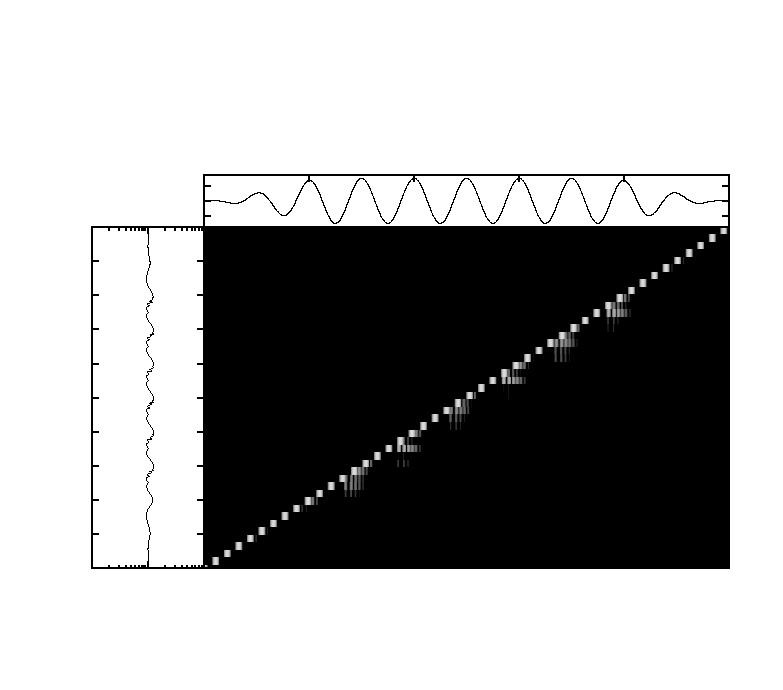
\includegraphics{c4_phase_vs_phase_low_2}}%
    \gplfronttext
  \end{picture}%
\endgroup
}
%    % 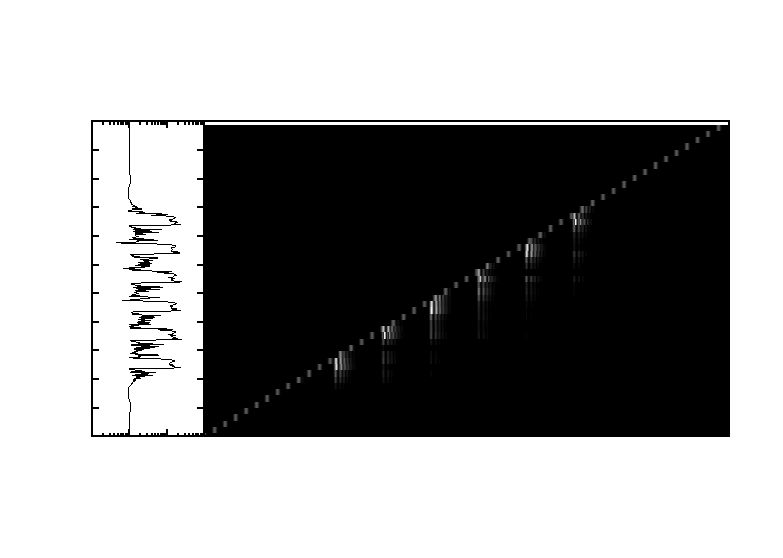
\includegraphics{c4_phase_vs_phase_1.t}}
%   \caption{
%   }
%  \label{fig:phase_vs_phase_low}
% \end{figure}

\subsection{The excess pressure as a function of the driving amplitude}\label{sec:phase_amp}



 \begin{figure}
   \centering
   \hspace*{-0.2cm}
   \subfloat[$\Ad = \unit{150}\kilo\pascal$]{
     \label{fig:excess_vs_phase::amp:compare::a}
     \includegraphics{c4_excess_amp_comp_a.0}}
   \subfloat[$\Ad = \unit{175}\kilo\pascal$]{
     \label{fig:excess_vs_phase::amp:compare::b}
     \includegraphics{c4_excess_amp_comp_b.0}}
   \subfloat[$\Ad = \unit{200}\kilo\pascal$]{
     \label{fig:excess_vs_phase::amp:compare::c}
     \includegraphics{c4_excess_amp_comp_c.0}}
    \caption{
      The excess scattering cross section for three different pressures.
      The diameter of the bubble is \unit{2}\micro\metre.
   }
   \label{fig:excess_intensity:amp:compare}
 \end{figure}


\begin{figure}
 \centering
% \subfloat[$n=1$]{
%  \label{fig:excess_vs_phase:a}
%  % GNUPLOT: LaTeX picture with Postscript
\begingroup
  \makeatletter
  \providecommand\color[2][]{%
    \GenericError{(gnuplot) \space\space\space\@spaces}{%
      Package color not loaded in conjunction with
      terminal option `colourtext'%
    }{See the gnuplot documentation for explanation.%
    }{Either use 'blacktext' in gnuplot or load the package
      color.sty in LaTeX.}%
    \renewcommand\color[2][]{}%
  }%
  \providecommand\includegraphics[2][]{%
    \GenericError{(gnuplot) \space\space\space\@spaces}{%
      Package graphicx or graphics not loaded%
    }{See the gnuplot documentation for explanation.%
    }{The gnuplot epslatex terminal needs graphicx.sty or graphics.sty.}%
    \renewcommand\includegraphics[2][]{}%
  }%
  \providecommand\rotatebox[2]{#2}%
  \@ifundefined{ifGPcolor}{%
    \newif\ifGPcolor
    \GPcolorfalse
  }{}%
  \@ifundefined{ifGPblacktext}{%
    \newif\ifGPblacktext
    \GPblacktexttrue
  }{}%
  % define a \g@addto@macro without @ in the name:
  \let\gplgaddtomacro\g@addto@macro
  % define empty templates for all commands taking text:
  \gdef\gplbacktext{}%
  \gdef\gplfronttext{}%
  \makeatother
  \ifGPblacktext
    % no textcolor at all
    \def\colorrgb#1{}%
    \def\colorgray#1{}%
  \else
    % gray or color?
    \ifGPcolor
      \def\colorrgb#1{\color[rgb]{#1}}%
      \def\colorgray#1{\color[gray]{#1}}%
      \expandafter\def\csname LTw\endcsname{\color{white}}%
      \expandafter\def\csname LTb\endcsname{\color{black}}%
      \expandafter\def\csname LTa\endcsname{\color{black}}%
      \expandafter\def\csname LT0\endcsname{\color[rgb]{1,0,0}}%
      \expandafter\def\csname LT1\endcsname{\color[rgb]{0,1,0}}%
      \expandafter\def\csname LT2\endcsname{\color[rgb]{0,0,1}}%
      \expandafter\def\csname LT3\endcsname{\color[rgb]{1,0,1}}%
      \expandafter\def\csname LT4\endcsname{\color[rgb]{0,1,1}}%
      \expandafter\def\csname LT5\endcsname{\color[rgb]{1,1,0}}%
      \expandafter\def\csname LT6\endcsname{\color[rgb]{0,0,0}}%
      \expandafter\def\csname LT7\endcsname{\color[rgb]{1,0.3,0}}%
      \expandafter\def\csname LT8\endcsname{\color[rgb]{0.5,0.5,0.5}}%
    \else
      % gray
      \def\colorrgb#1{\color{black}}%
      \def\colorgray#1{\color[gray]{#1}}%
      \expandafter\def\csname LTw\endcsname{\color{white}}%
      \expandafter\def\csname LTb\endcsname{\color{black}}%
      \expandafter\def\csname LTa\endcsname{\color{black}}%
      \expandafter\def\csname LT0\endcsname{\color{black}}%
      \expandafter\def\csname LT1\endcsname{\color{black}}%
      \expandafter\def\csname LT2\endcsname{\color{black}}%
      \expandafter\def\csname LT3\endcsname{\color{black}}%
      \expandafter\def\csname LT4\endcsname{\color{black}}%
      \expandafter\def\csname LT5\endcsname{\color{black}}%
      \expandafter\def\csname LT6\endcsname{\color{black}}%
      \expandafter\def\csname LT7\endcsname{\color{black}}%
      \expandafter\def\csname LT8\endcsname{\color{black}}%
    \fi
  \fi
  \setlength{\unitlength}{0.0500bp}%
  \begin{picture}(7200.00,5040.00)%
    \gplgaddtomacro\gplbacktext{%
      \csname LTb\endcsname%
      \put(588,1008){\makebox(0,0)[r]{\strut{}0}}%
      \put(588,1283){\makebox(0,0)[r]{\strut{}$2\pi$}}%
      \put(588,1558){\makebox(0,0)[r]{\strut{}$4\pi$}}%
      \put(588,1833){\makebox(0,0)[r]{\strut{}$6\pi$}}%
      \put(588,2108){\makebox(0,0)[r]{\strut{}$8\pi$}}%
      \put(588,2383){\makebox(0,0)[r]{\strut{}$10\pi$}}%
      \put(588,2657){\makebox(0,0)[r]{\strut{}$12\pi$}}%
      \put(588,2932){\makebox(0,0)[r]{\strut{}$14\pi$}}%
      \put(588,3207){\makebox(0,0)[r]{\strut{}$16\pi$}}%
      \put(588,3482){\makebox(0,0)[r]{\strut{}$18\pi$}}%
      \put(588,3757){\makebox(0,0)[r]{\strut{}$20\pi$}}%
      \put(720,788){\makebox(0,0){\strut{}$10^{0}$}}%
      \put(1080,788){\makebox(0,0){\strut{}$10^{1}$}}%
      \put(1440,788){\makebox(0,0){\strut{}$10^{2}$}}%
      \put(1800,788){\makebox(0,0){\strut{}$10^{3}$}}%
      \put(-50,2520){\rotatebox{90}{\makebox(0,0){\strut{}sampled driving phase, $\phi_{d0}$}}}%
      \put(1260,458){\makebox(0,0){\strut{}driving phase, $\phi_d$}}%
    }%
    \gplgaddtomacro\gplfronttext{%
    }%
    \gplgaddtomacro\gplbacktext{%
    }%
    \gplgaddtomacro\gplfronttext{%
      \csname LTb\endcsname%
      \put(1801,641){\makebox(0,0){\strut{}0}}%
      \put(2259,641){\makebox(0,0){\strut{}$2\pi$}}%
      \put(2717,641){\makebox(0,0){\strut{}$4\pi$}}%
      \put(3175,641){\makebox(0,0){\strut{}$6\pi$}}%
      \put(3633,641){\makebox(0,0){\strut{}$8\pi$}}%
      \put(4091,641){\makebox(0,0){\strut{}$10\pi$}}%
      \put(4549,641){\makebox(0,0){\strut{}$12\pi$}}%
      \put(5007,641){\makebox(0,0){\strut{}$14\pi$}}%
      \put(5465,641){\makebox(0,0){\strut{}$16\pi$}}%
      \put(5923,641){\makebox(0,0){\strut{}$18\pi$}}%
      \put(6381,641){\makebox(0,0){\strut{}$20\pi$}}%
      \put(4320,311){\makebox(0,0){\strut{}driving phase, $\phi_d$}}%
    }%
    \gplbacktext
    \put(0,0){\includegraphics{c4_phase_vs_phase_1}}%
    \gplfronttext
  \end{picture}%
\endgroup
}
% \subfloat[$n=1$]{
%   \label{fig:excess_vs_phase:b}
 % GNUPLOT: LaTeX picture with Postscript
\begingroup
  \makeatletter
  \providecommand\color[2][]{%
    \GenericError{(gnuplot) \space\space\space\@spaces}{%
      Package color not loaded in conjunction with
      terminal option `colourtext'%
    }{See the gnuplot documentation for explanation.%
    }{Either use 'blacktext' in gnuplot or load the package
      color.sty in LaTeX.}%
    \renewcommand\color[2][]{}%
  }%
  \providecommand\includegraphics[2][]{%
    \GenericError{(gnuplot) \space\space\space\@spaces}{%
      Package graphicx or graphics not loaded%
    }{See the gnuplot documentation for explanation.%
    }{The gnuplot epslatex terminal needs graphicx.sty or graphics.sty.}%
    \renewcommand\includegraphics[2][]{}%
  }%
  \providecommand\rotatebox[2]{#2}%
  \@ifundefined{ifGPcolor}{%
    \newif\ifGPcolor
    \GPcolorfalse
  }{}%
  \@ifundefined{ifGPblacktext}{%
    \newif\ifGPblacktext
    \GPblacktexttrue
  }{}%
  % define a \g@addto@macro without @ in the name:
  \let\gplgaddtomacro\g@addto@macro
  % define empty templates for all commands taking text:
  \gdef\gplbacktext{}%
  \gdef\gplfronttext{}%
  \makeatother
  \ifGPblacktext
    % no textcolor at all
    \def\colorrgb#1{}%
    \def\colorgray#1{}%
  \else
    % gray or color?
    \ifGPcolor
      \def\colorrgb#1{\color[rgb]{#1}}%
      \def\colorgray#1{\color[gray]{#1}}%
      \expandafter\def\csname LTw\endcsname{\color{white}}%
      \expandafter\def\csname LTb\endcsname{\color{black}}%
      \expandafter\def\csname LTa\endcsname{\color{black}}%
      \expandafter\def\csname LT0\endcsname{\color[rgb]{1,0,0}}%
      \expandafter\def\csname LT1\endcsname{\color[rgb]{0,1,0}}%
      \expandafter\def\csname LT2\endcsname{\color[rgb]{0,0,1}}%
      \expandafter\def\csname LT3\endcsname{\color[rgb]{1,0,1}}%
      \expandafter\def\csname LT4\endcsname{\color[rgb]{0,1,1}}%
      \expandafter\def\csname LT5\endcsname{\color[rgb]{1,1,0}}%
      \expandafter\def\csname LT6\endcsname{\color[rgb]{0,0,0}}%
      \expandafter\def\csname LT7\endcsname{\color[rgb]{1,0.3,0}}%
      \expandafter\def\csname LT8\endcsname{\color[rgb]{0.5,0.5,0.5}}%
    \else
      % gray
      \def\colorrgb#1{\color{black}}%
      \def\colorgray#1{\color[gray]{#1}}%
      \expandafter\def\csname LTw\endcsname{\color{white}}%
      \expandafter\def\csname LTb\endcsname{\color{black}}%
      \expandafter\def\csname LTa\endcsname{\color{black}}%
      \expandafter\def\csname LT0\endcsname{\color{black}}%
      \expandafter\def\csname LT1\endcsname{\color{black}}%
      \expandafter\def\csname LT2\endcsname{\color{black}}%
      \expandafter\def\csname LT3\endcsname{\color{black}}%
      \expandafter\def\csname LT4\endcsname{\color{black}}%
      \expandafter\def\csname LT5\endcsname{\color{black}}%
      \expandafter\def\csname LT6\endcsname{\color{black}}%
      \expandafter\def\csname LT7\endcsname{\color{black}}%
      \expandafter\def\csname LT8\endcsname{\color{black}}%
    \fi
  \fi
  \setlength{\unitlength}{0.0500bp}%
  \begin{picture}(7200.00,5040.00)%
    \gplgaddtomacro\gplbacktext{%
      \csname LTb\endcsname%
      \put(588,1008){\makebox(0,0)[r]{\strut{}0}}%
      \put(588,1283){\makebox(0,0)[r]{\strut{}$2\pi$}}%
      \put(588,1558){\makebox(0,0)[r]{\strut{}$4\pi$}}%
      \put(588,1833){\makebox(0,0)[r]{\strut{}$6\pi$}}%
      \put(588,2108){\makebox(0,0)[r]{\strut{}$8\pi$}}%
      \put(588,2383){\makebox(0,0)[r]{\strut{}$10\pi$}}%
      \put(588,2657){\makebox(0,0)[r]{\strut{}$12\pi$}}%
      \put(588,2932){\makebox(0,0)[r]{\strut{}$14\pi$}}%
      \put(588,3207){\makebox(0,0)[r]{\strut{}$16\pi$}}%
      \put(588,3482){\makebox(0,0)[r]{\strut{}$18\pi$}}%
      \put(588,3757){\makebox(0,0)[r]{\strut{}$20\pi$}}%
      \put(720,788){\makebox(0,0){\strut{}$10^{0}$}}%
      \put(1080,788){\makebox(0,0){\strut{}$10^{1}$}}%
      \put(1440,788){\makebox(0,0){\strut{}$10^{2}$}}%
      \put(1800,788){\makebox(0,0){\strut{}$10^{3}$}}%
      \put(-50,2520){\rotatebox{90}{\makebox(0,0){\strut{}sampled driving phase, $\phi_{d0}$}}}%
      \put(1260,293){\makebox(0,0){\strut{}$\sigma_{ex}$}}%
    }%
    \gplgaddtomacro\gplfronttext{%
    }%
    \gplgaddtomacro\gplbacktext{%
    }%
    \gplgaddtomacro\gplfronttext{%
      \csname LTb\endcsname%
      \put(1801,641){\makebox(0,0){\strut{}0}}%
      \put(2259,641){\makebox(0,0){\strut{}$2\pi$}}%
      \put(2717,641){\makebox(0,0){\strut{}$4\pi$}}%
      \put(3175,641){\makebox(0,0){\strut{}$6\pi$}}%
      \put(3633,641){\makebox(0,0){\strut{}$8\pi$}}%
      \put(4091,641){\makebox(0,0){\strut{}$10\pi$}}%
      \put(4549,641){\makebox(0,0){\strut{}$12\pi$}}%
      \put(5007,641){\makebox(0,0){\strut{}$14\pi$}}%
      \put(5465,641){\makebox(0,0){\strut{}$16\pi$}}%
      \put(5923,641){\makebox(0,0){\strut{}$18\pi$}}%
      \put(6381,641){\makebox(0,0){\strut{}$20\pi$}}%
      \put(4320,147){\makebox(0,0){\strut{}$\sigma_{ex}$}}%
    }%
    \gplbacktext
    \put(0,0){\includegraphics{c4_phase_vs_phase_2}}%
    \gplfronttext
  \end{picture}%
\endgroup

%}
   % \includegraphics{c4_phase_vs_phase_1.t}}
  \caption{
The excess pressure and the excess scattering cross section as a function of $\phidi$ and $\phid$
for a \unit{2}\micro\metre-diameter bubble pulsated with a driving pressure of  \unit{175}\kilo\pascal.
  }
 \label{fig:excess_vs_phase_1_75}
\end{figure}

The driving amplitude strongly affects the excess scatter.
In \figref{excess_intensity:amp:compare} the excess scattering cross section 
is plotted a driving wave of \unit{175}\kilo\pascal, \unit{200}\kilo\pascal,
in addition to the \unit{150}\kilo\pascal\ evaluated in \secref{excess_phase}.

At the low pressure of \unit{150}\kilo\pascal\  the excess scattering cross section is periodic 
with a near sinusoid. 
Even though the response is already  harmonic
the perturbation to the  phase-space orbit rapidly decays,
as is seen by the short lived (less than 1 cycle of the driving wave)
excess pressure signals in \figref{excess_vs_phase}.

At the higher pressure of \unit{175}\kilo\pascal\ the scattering is still periodic
but is an order of magnitude greater when the bubble is expanded to when it is compressed.
This is not due, unfortunately, to a huge phase-dependence in the scattering of the bubble,
but rather due the inclusion of phantom bubbles in $\excessI$, which  seen  in \figref{excess_vs_phase_1_75}.
The preferential appearance of phantom bubbles  in the expansion phase was anticipated in \secref{reducing_perturbation}.

At the higher still pressure of \unit{200}\kilo\pascal\ the scattering is swamped by phantom bubbles,
and while the scattering is still broadly periodic, it has become somewhat unpredictable,
varying widely for very closely related sampled phases.




\begin{figure}
 \centering
 \subfloat[$a = \unit{100}\nano\metre$]{
   \label{fig:phase_amp:a}
   % GNUPLOT: LaTeX picture with Postscript
\begingroup
  \makeatletter
  \providecommand\color[2][]{%
    \GenericError{(gnuplot) \space\space\space\@spaces}{%
      Package color not loaded in conjunction with
      terminal option `colourtext'%
    }{See the gnuplot documentation for explanation.%
    }{Either use 'blacktext' in gnuplot or load the package
      color.sty in LaTeX.}%
    \renewcommand\color[2][]{}%
  }%
  \providecommand\includegraphics[2][]{%
    \GenericError{(gnuplot) \space\space\space\@spaces}{%
      Package graphicx or graphics not loaded%
    }{See the gnuplot documentation for explanation.%
    }{The gnuplot epslatex terminal needs graphicx.sty or graphics.sty.}%
    \renewcommand\includegraphics[2][]{}%
  }%
  \providecommand\rotatebox[2]{#2}%
  \@ifundefined{ifGPcolor}{%
    \newif\ifGPcolor
    \GPcolorfalse
  }{}%
  \@ifundefined{ifGPblacktext}{%
    \newif\ifGPblacktext
    \GPblacktexttrue
  }{}%
  % define a \g@addto@macro without @ in the name:
  \let\gplgaddtomacro\g@addto@macro
  % define empty templates for all commands taking text:
  \gdef\gplbacktext{}%
  \gdef\gplfronttext{}%
  \makeatother
  \ifGPblacktext
    % no textcolor at all
    \def\colorrgb#1{}%
    \def\colorgray#1{}%
  \else
    % gray or color?
    \ifGPcolor
      \def\colorrgb#1{\color[rgb]{#1}}%
      \def\colorgray#1{\color[gray]{#1}}%
      \expandafter\def\csname LTw\endcsname{\color{white}}%
      \expandafter\def\csname LTb\endcsname{\color{black}}%
      \expandafter\def\csname LTa\endcsname{\color{black}}%
      \expandafter\def\csname LT0\endcsname{\color[rgb]{1,0,0}}%
      \expandafter\def\csname LT1\endcsname{\color[rgb]{0,1,0}}%
      \expandafter\def\csname LT2\endcsname{\color[rgb]{0,0,1}}%
      \expandafter\def\csname LT3\endcsname{\color[rgb]{1,0,1}}%
      \expandafter\def\csname LT4\endcsname{\color[rgb]{0,1,1}}%
      \expandafter\def\csname LT5\endcsname{\color[rgb]{1,1,0}}%
      \expandafter\def\csname LT6\endcsname{\color[rgb]{0,0,0}}%
      \expandafter\def\csname LT7\endcsname{\color[rgb]{1,0.3,0}}%
      \expandafter\def\csname LT8\endcsname{\color[rgb]{0.5,0.5,0.5}}%
    \else
      % gray
      \def\colorrgb#1{\color{black}}%
      \def\colorgray#1{\color[gray]{#1}}%
      \expandafter\def\csname LTw\endcsname{\color{white}}%
      \expandafter\def\csname LTb\endcsname{\color{black}}%
      \expandafter\def\csname LTa\endcsname{\color{black}}%
      \expandafter\def\csname LT0\endcsname{\color{black}}%
      \expandafter\def\csname LT1\endcsname{\color{black}}%
      \expandafter\def\csname LT2\endcsname{\color{black}}%
      \expandafter\def\csname LT3\endcsname{\color{black}}%
      \expandafter\def\csname LT4\endcsname{\color{black}}%
      \expandafter\def\csname LT5\endcsname{\color{black}}%
      \expandafter\def\csname LT6\endcsname{\color{black}}%
      \expandafter\def\csname LT7\endcsname{\color{black}}%
      \expandafter\def\csname LT8\endcsname{\color{black}}%
    \fi
  \fi
  \setlength{\unitlength}{0.0500bp}%
  \begin{picture}(7200.00,5040.00)%
    \gplgaddtomacro\gplbacktext{%
    }%
    \gplgaddtomacro\gplfronttext{%
      \csname LTb\endcsname%
      \put(1840,800){\makebox(0,0){\strut{} 0.05}}%
      \put(2678,800){\makebox(0,0){\strut{} 0.1}}%
      \put(3517,800){\makebox(0,0){\strut{} 0.15}}%
      \put(4354,800){\makebox(0,0){\strut{} 0.2}}%
      \put(5192,800){\makebox(0,0){\strut{} 0.25}}%
      \put(6030,800){\makebox(0,0){\strut{} 0.3}}%
      \put(3600,470){\makebox(0,0){\strut{}driving pressure (MPa)}}%
      \put(998,1086){\makebox(0,0)[r]{\strut{}0}}%
      \put(998,1704){\makebox(0,0)[r]{\strut{}4$\pi$}}%
      \put(998,2322){\makebox(0,0)[r]{\strut{}8$\pi$}}%
      \put(998,2938){\makebox(0,0)[r]{\strut{}12$\pi$}}%
      \put(998,3556){\makebox(0,0)[r]{\strut{}16$\pi$}}%
      \put(998,4174){\makebox(0,0)[r]{\strut{}20$\pi$}}%
      \put(338,2630){\rotatebox{90}{\makebox(0,0){\strut{}phase, $\phi_d$}}}%
      \put(6527,1085){\makebox(0,0)[l]{\strut{}$10^{-3}$}}%
      \put(6527,2629){\makebox(0,0)[l]{\strut{}$10^{-2}$}}%
      \put(6527,4174){\makebox(0,0)[l]{\strut{}$10^{-1}$}}%
      \put(7122,2629){\rotatebox{90}{\makebox(0,0){\strut{}$\sigma_{ex}$}}}%
    }%
    \gplbacktext
    \put(0,0){\includegraphics{c4_phase_amp_0_1}}%
    \gplfronttext
  \end{picture}%
\endgroup
}
 \subfloat[$a = \unit{1}\micro\metre$]{
   \label{fig:phase_amp:b}
   % GNUPLOT: LaTeX picture with Postscript
\begingroup
  \makeatletter
  \providecommand\color[2][]{%
    \GenericError{(gnuplot) \space\space\space\@spaces}{%
      Package color not loaded in conjunction with
      terminal option `colourtext'%
    }{See the gnuplot documentation for explanation.%
    }{Either use 'blacktext' in gnuplot or load the package
      color.sty in LaTeX.}%
    \renewcommand\color[2][]{}%
  }%
  \providecommand\includegraphics[2][]{%
    \GenericError{(gnuplot) \space\space\space\@spaces}{%
      Package graphicx or graphics not loaded%
    }{See the gnuplot documentation for explanation.%
    }{The gnuplot epslatex terminal needs graphicx.sty or graphics.sty.}%
    \renewcommand\includegraphics[2][]{}%
  }%
  \providecommand\rotatebox[2]{#2}%
  \@ifundefined{ifGPcolor}{%
    \newif\ifGPcolor
    \GPcolorfalse
  }{}%
  \@ifundefined{ifGPblacktext}{%
    \newif\ifGPblacktext
    \GPblacktexttrue
  }{}%
  % define a \g@addto@macro without @ in the name:
  \let\gplgaddtomacro\g@addto@macro
  % define empty templates for all commands taking text:
  \gdef\gplbacktext{}%
  \gdef\gplfronttext{}%
  \makeatother
  \ifGPblacktext
    % no textcolor at all
    \def\colorrgb#1{}%
    \def\colorgray#1{}%
  \else
    % gray or color?
    \ifGPcolor
      \def\colorrgb#1{\color[rgb]{#1}}%
      \def\colorgray#1{\color[gray]{#1}}%
      \expandafter\def\csname LTw\endcsname{\color{white}}%
      \expandafter\def\csname LTb\endcsname{\color{black}}%
      \expandafter\def\csname LTa\endcsname{\color{black}}%
      \expandafter\def\csname LT0\endcsname{\color[rgb]{1,0,0}}%
      \expandafter\def\csname LT1\endcsname{\color[rgb]{0,1,0}}%
      \expandafter\def\csname LT2\endcsname{\color[rgb]{0,0,1}}%
      \expandafter\def\csname LT3\endcsname{\color[rgb]{1,0,1}}%
      \expandafter\def\csname LT4\endcsname{\color[rgb]{0,1,1}}%
      \expandafter\def\csname LT5\endcsname{\color[rgb]{1,1,0}}%
      \expandafter\def\csname LT6\endcsname{\color[rgb]{0,0,0}}%
      \expandafter\def\csname LT7\endcsname{\color[rgb]{1,0.3,0}}%
      \expandafter\def\csname LT8\endcsname{\color[rgb]{0.5,0.5,0.5}}%
    \else
      % gray
      \def\colorrgb#1{\color{black}}%
      \def\colorgray#1{\color[gray]{#1}}%
      \expandafter\def\csname LTw\endcsname{\color{white}}%
      \expandafter\def\csname LTb\endcsname{\color{black}}%
      \expandafter\def\csname LTa\endcsname{\color{black}}%
      \expandafter\def\csname LT0\endcsname{\color{black}}%
      \expandafter\def\csname LT1\endcsname{\color{black}}%
      \expandafter\def\csname LT2\endcsname{\color{black}}%
      \expandafter\def\csname LT3\endcsname{\color{black}}%
      \expandafter\def\csname LT4\endcsname{\color{black}}%
      \expandafter\def\csname LT5\endcsname{\color{black}}%
      \expandafter\def\csname LT6\endcsname{\color{black}}%
      \expandafter\def\csname LT7\endcsname{\color{black}}%
      \expandafter\def\csname LT8\endcsname{\color{black}}%
    \fi
  \fi
  \setlength{\unitlength}{0.0500bp}%
  \begin{picture}(7200.00,5040.00)%
    \gplgaddtomacro\gplbacktext{%
    }%
    \gplgaddtomacro\gplfronttext{%
      \csname LTb\endcsname%
      \put(1840,800){\makebox(0,0){\strut{} 0.05}}%
      \put(2678,800){\makebox(0,0){\strut{} 0.1}}%
      \put(3517,800){\makebox(0,0){\strut{} 0.15}}%
      \put(4354,800){\makebox(0,0){\strut{} 0.2}}%
      \put(5192,800){\makebox(0,0){\strut{} 0.25}}%
      \put(6030,800){\makebox(0,0){\strut{} 0.3}}%
      \put(3600,470){\makebox(0,0){\strut{}driving pressure (MPa)}}%
      \put(998,1086){\makebox(0,0)[r]{\strut{}0}}%
      \put(998,1704){\makebox(0,0)[r]{\strut{}4$\pi$}}%
      \put(998,2322){\makebox(0,0)[r]{\strut{}8$\pi$}}%
      \put(998,2938){\makebox(0,0)[r]{\strut{}12$\pi$}}%
      \put(998,3556){\makebox(0,0)[r]{\strut{}16$\pi$}}%
      \put(998,4174){\makebox(0,0)[r]{\strut{}20$\pi$}}%
      \put(338,2630){\rotatebox{90}{\makebox(0,0){\strut{}phase, $\phi_d$}}}%
      \put(6527,1085){\makebox(0,0)[l]{\strut{}$10^{0}$}}%
      \put(6527,1526){\makebox(0,0)[l]{\strut{}$10^{1}$}}%
      \put(6527,1967){\makebox(0,0)[l]{\strut{}$10^{2}$}}%
      \put(6527,2408){\makebox(0,0)[l]{\strut{}$10^{3}$}}%
      \put(6527,2850){\makebox(0,0)[l]{\strut{}$10^{4}$}}%
      \put(6527,3291){\makebox(0,0)[l]{\strut{}$10^{5}$}}%
      \put(6527,3732){\makebox(0,0)[l]{\strut{}$10^{6}$}}%
      \put(6527,4174){\makebox(0,0)[l]{\strut{}$10^{7}$}}%
      \put(6990,2629){\rotatebox{90}{\makebox(0,0){\strut{}$\sigma_{ex}$}}}%
    }%
    \gplbacktext
    \put(0,0){\includegraphics{c4_phase_amp_1}}%
    \gplfronttext
  \end{picture}%
\endgroup
}
   % \includegraphics{c4_phase_vs_phase_1.t}}
  \caption{
    The excess scattering cross section as a function of the driving phase and the driving pressure
    for two different bubble radii.
  }
 \label{fig:phase_amp}
\end{figure}

To understand how the driving amplitude affects the scattering more generally,
we plot  $\excessI$ as a function of the phase $\phidi$ and the driving amplitude.
This is calculated for two bubble radii in \figref{phase_amp}.
In \subref{fig:phase_amp:a} the radius is \unit{0.1}\micro\metre\ and
in \subref{fig:phase_amp:b} the radius is \unit{1.0}\micro\metre. %  - as was used before.
For small bubbles the phase relationship of the scattering is both simple and uniform for all driving pressures between 0 and \unit{300}\kilo\pascal,
when driven at \unit{0.5}\mega\hertz.
However, the situation changes radically at the larger radius in \figref{phase_amp:b}.





\subsection{The excess pressure as a function of the radius}

\begin{figure}
 \centering
  % GNUPLOT: LaTeX picture with Postscript
\begingroup
  \makeatletter
  \providecommand\color[2][]{%
    \GenericError{(gnuplot) \space\space\space\@spaces}{%
      Package color not loaded in conjunction with
      terminal option `colourtext'%
    }{See the gnuplot documentation for explanation.%
    }{Either use 'blacktext' in gnuplot or load the package
      color.sty in LaTeX.}%
    \renewcommand\color[2][]{}%
  }%
  \providecommand\includegraphics[2][]{%
    \GenericError{(gnuplot) \space\space\space\@spaces}{%
      Package graphicx or graphics not loaded%
    }{See the gnuplot documentation for explanation.%
    }{The gnuplot epslatex terminal needs graphicx.sty or graphics.sty.}%
    \renewcommand\includegraphics[2][]{}%
  }%
  \providecommand\rotatebox[2]{#2}%
  \@ifundefined{ifGPcolor}{%
    \newif\ifGPcolor
    \GPcolorfalse
  }{}%
  \@ifundefined{ifGPblacktext}{%
    \newif\ifGPblacktext
    \GPblacktexttrue
  }{}%
  % define a \g@addto@macro without @ in the name:
  \let\gplgaddtomacro\g@addto@macro
  % define empty templates for all commands taking text:
  \gdef\gplbacktext{}%
  \gdef\gplfronttext{}%
  \makeatother
  \ifGPblacktext
    % no textcolor at all
    \def\colorrgb#1{}%
    \def\colorgray#1{}%
  \else
    % gray or color?
    \ifGPcolor
      \def\colorrgb#1{\color[rgb]{#1}}%
      \def\colorgray#1{\color[gray]{#1}}%
      \expandafter\def\csname LTw\endcsname{\color{white}}%
      \expandafter\def\csname LTb\endcsname{\color{black}}%
      \expandafter\def\csname LTa\endcsname{\color{black}}%
      \expandafter\def\csname LT0\endcsname{\color[rgb]{1,0,0}}%
      \expandafter\def\csname LT1\endcsname{\color[rgb]{0,1,0}}%
      \expandafter\def\csname LT2\endcsname{\color[rgb]{0,0,1}}%
      \expandafter\def\csname LT3\endcsname{\color[rgb]{1,0,1}}%
      \expandafter\def\csname LT4\endcsname{\color[rgb]{0,1,1}}%
      \expandafter\def\csname LT5\endcsname{\color[rgb]{1,1,0}}%
      \expandafter\def\csname LT6\endcsname{\color[rgb]{0,0,0}}%
      \expandafter\def\csname LT7\endcsname{\color[rgb]{1,0.3,0}}%
      \expandafter\def\csname LT8\endcsname{\color[rgb]{0.5,0.5,0.5}}%
    \else
      % gray
      \def\colorrgb#1{\color{black}}%
      \def\colorgray#1{\color[gray]{#1}}%
      \expandafter\def\csname LTw\endcsname{\color{white}}%
      \expandafter\def\csname LTb\endcsname{\color{black}}%
      \expandafter\def\csname LTa\endcsname{\color{black}}%
      \expandafter\def\csname LT0\endcsname{\color{black}}%
      \expandafter\def\csname LT1\endcsname{\color{black}}%
      \expandafter\def\csname LT2\endcsname{\color{black}}%
      \expandafter\def\csname LT3\endcsname{\color{black}}%
      \expandafter\def\csname LT4\endcsname{\color{black}}%
      \expandafter\def\csname LT5\endcsname{\color{black}}%
      \expandafter\def\csname LT6\endcsname{\color{black}}%
      \expandafter\def\csname LT7\endcsname{\color{black}}%
      \expandafter\def\csname LT8\endcsname{\color{black}}%
    \fi
  \fi
  \setlength{\unitlength}{0.0500bp}%
  \begin{picture}(7200.00,5040.00)%
    \gplgaddtomacro\gplbacktext{%
    }%
    \gplgaddtomacro\gplfronttext{%
      \csname LTb\endcsname%
      \put(1425,800){\makebox(0,0){\strut{} 0.2}}%
      \put(1937,800){\makebox(0,0){\strut{} 0.4}}%
      \put(2449,800){\makebox(0,0){\strut{} 0.6}}%
      \put(2961,800){\makebox(0,0){\strut{} 0.8}}%
      \put(3473,800){\makebox(0,0){\strut{} 1}}%
      \put(3983,800){\makebox(0,0){\strut{} 1.2}}%
      \put(4495,800){\makebox(0,0){\strut{} 1.4}}%
      \put(5007,800){\makebox(0,0){\strut{} 1.6}}%
      \put(5519,800){\makebox(0,0){\strut{} 1.8}}%
      \put(6030,800){\makebox(0,0){\strut{} 2}}%
      \put(3600,470){\makebox(0,0){\strut{}radius ($\mu m$)}}%
      \put(998,1086){\makebox(0,0)[r]{\strut{}0}}%
      \put(998,1704){\makebox(0,0)[r]{\strut{}4$\pi$}}%
      \put(998,2322){\makebox(0,0)[r]{\strut{}8$\pi$}}%
      \put(998,2938){\makebox(0,0)[r]{\strut{}12$\pi$}}%
      \put(998,3556){\makebox(0,0)[r]{\strut{}16$\pi$}}%
      \put(998,4174){\makebox(0,0)[r]{\strut{}20$\pi$}}%
      \put(338,2630){\rotatebox{90}{\makebox(0,0){\strut{}phase, $\phi_d$}}}%
      \put(6527,1085){\makebox(0,0)[l]{\strut{}$10^{-2}$}}%
      \put(6527,1526){\makebox(0,0)[l]{\strut{}$10^{-1}$}}%
      \put(6527,1967){\makebox(0,0)[l]{\strut{}$10^{0}$}}%
      \put(6527,2408){\makebox(0,0)[l]{\strut{}$10^{1}$}}%
      \put(6527,2850){\makebox(0,0)[l]{\strut{}$10^{2}$}}%
      \put(6527,3291){\makebox(0,0)[l]{\strut{}$10^{3}$}}%
      \put(6527,3732){\makebox(0,0)[l]{\strut{}$10^{4}$}}%
      \put(6527,4174){\makebox(0,0)[l]{\strut{}$10^{5}$}}%
      \put(7122,2629){\rotatebox{90}{\makebox(0,0){\strut{}$\sigma_{ex}$}}}%
    }%
    \gplbacktext
    \put(0,0){\includegraphics{c4_phase_radial_1}}%
    \gplfronttext
  \end{picture}%
\endgroup

   % \includegraphics{c4_phase_vs_phase_1.t}}
  \caption{
    The excess pressure scattering as a function of the driving phase and the radius.
  }
 \label{fig:phase_radial}
\end{figure}

To understand the role of the bubble's radius of the excess scattering cross section,
$\excessI$ is plotted as a function of $\phidi$ and $a$ in \figref{phase_radial}.

The most interesting feature of this plot is the fork in the phase dependence for bubbles with a radius of about \unit{0.3}\micro\metre.
Below this radius the scattering is maximal when $\phidi$ is an odd multiple of $\pi$,
or when the bubble is at its largest size.
Above  \unit{0.3}\micro\metre\ the scattering is maximal when $\phidi$ is an even multiple of $\pi$,
or when the bubble is small.
Such $\pi$ radian changes in phase occur at resonance,
and we saw in \figref{DeltaPhi} that a \unit{300}\nano\metre\ bubble is resonant at \unit{20}\mega\hertz.
When the bubble is below \unit{0.3}\micro\metre\ the scattering increases simply due to the bubble's increased size.
Above the resonance the scattering is increased when the bubble is shrunk back towards resonance.

Radii above \unit{1.2}\micro\metre\ start to approach the resonance of the driving wave.
The phase space trajectories then become less stable to perturbations by the imaging wave and the scattering
starts to increase again when the bubble is expanded.
Above \unit{2}\micro\metre\ the phase response to the driving wave starts to shift with this second resonance,
and the phase relation breaks down.


% \subsection{The excess pressure as a function of driving frequency}\label{sec:phase_amp}


% \begin{figure}
%  \centering
%   % GNUPLOT: LaTeX picture with Postscript
\begingroup
  \makeatletter
  \providecommand\color[2][]{%
    \GenericError{(gnuplot) \space\space\space\@spaces}{%
      Package color not loaded in conjunction with
      terminal option `colourtext'%
    }{See the gnuplot documentation for explanation.%
    }{Either use 'blacktext' in gnuplot or load the package
      color.sty in LaTeX.}%
    \renewcommand\color[2][]{}%
  }%
  \providecommand\includegraphics[2][]{%
    \GenericError{(gnuplot) \space\space\space\@spaces}{%
      Package graphicx or graphics not loaded%
    }{See the gnuplot documentation for explanation.%
    }{The gnuplot epslatex terminal needs graphicx.sty or graphics.sty.}%
    \renewcommand\includegraphics[2][]{}%
  }%
  \providecommand\rotatebox[2]{#2}%
  \@ifundefined{ifGPcolor}{%
    \newif\ifGPcolor
    \GPcolorfalse
  }{}%
  \@ifundefined{ifGPblacktext}{%
    \newif\ifGPblacktext
    \GPblacktexttrue
  }{}%
  % define a \g@addto@macro without @ in the name:
  \let\gplgaddtomacro\g@addto@macro
  % define empty templates for all commands taking text:
  \gdef\gplbacktext{}%
  \gdef\gplfronttext{}%
  \makeatother
  \ifGPblacktext
    % no textcolor at all
    \def\colorrgb#1{}%
    \def\colorgray#1{}%
  \else
    % gray or color?
    \ifGPcolor
      \def\colorrgb#1{\color[rgb]{#1}}%
      \def\colorgray#1{\color[gray]{#1}}%
      \expandafter\def\csname LTw\endcsname{\color{white}}%
      \expandafter\def\csname LTb\endcsname{\color{black}}%
      \expandafter\def\csname LTa\endcsname{\color{black}}%
      \expandafter\def\csname LT0\endcsname{\color[rgb]{1,0,0}}%
      \expandafter\def\csname LT1\endcsname{\color[rgb]{0,1,0}}%
      \expandafter\def\csname LT2\endcsname{\color[rgb]{0,0,1}}%
      \expandafter\def\csname LT3\endcsname{\color[rgb]{1,0,1}}%
      \expandafter\def\csname LT4\endcsname{\color[rgb]{0,1,1}}%
      \expandafter\def\csname LT5\endcsname{\color[rgb]{1,1,0}}%
      \expandafter\def\csname LT6\endcsname{\color[rgb]{0,0,0}}%
      \expandafter\def\csname LT7\endcsname{\color[rgb]{1,0.3,0}}%
      \expandafter\def\csname LT8\endcsname{\color[rgb]{0.5,0.5,0.5}}%
    \else
      % gray
      \def\colorrgb#1{\color{black}}%
      \def\colorgray#1{\color[gray]{#1}}%
      \expandafter\def\csname LTw\endcsname{\color{white}}%
      \expandafter\def\csname LTb\endcsname{\color{black}}%
      \expandafter\def\csname LTa\endcsname{\color{black}}%
      \expandafter\def\csname LT0\endcsname{\color{black}}%
      \expandafter\def\csname LT1\endcsname{\color{black}}%
      \expandafter\def\csname LT2\endcsname{\color{black}}%
      \expandafter\def\csname LT3\endcsname{\color{black}}%
      \expandafter\def\csname LT4\endcsname{\color{black}}%
      \expandafter\def\csname LT5\endcsname{\color{black}}%
      \expandafter\def\csname LT6\endcsname{\color{black}}%
      \expandafter\def\csname LT7\endcsname{\color{black}}%
      \expandafter\def\csname LT8\endcsname{\color{black}}%
    \fi
  \fi
  \setlength{\unitlength}{0.0500bp}%
  \begin{picture}(7200.00,5040.00)%
    \gplgaddtomacro\gplbacktext{%
    }%
    \gplgaddtomacro\gplfronttext{%
      \csname LTb\endcsname%
      \put(1170,800){\makebox(0,0){\strut{} 0.2}}%
      \put(1710,800){\makebox(0,0){\strut{} 0.4}}%
      \put(2250,800){\makebox(0,0){\strut{} 0.6}}%
      \put(2790,800){\makebox(0,0){\strut{} 0.8}}%
      \put(3330,800){\makebox(0,0){\strut{} 1}}%
      \put(3870,800){\makebox(0,0){\strut{} 1.2}}%
      \put(4410,800){\makebox(0,0){\strut{} 1.4}}%
      \put(4950,800){\makebox(0,0){\strut{} 1.6}}%
      \put(5490,800){\makebox(0,0){\strut{} 1.8}}%
      \put(6030,800){\makebox(0,0){\strut{} 2}}%
      \put(3600,470){\makebox(0,0){\strut{}radius ($\mu m$)}}%
      \put(998,1086){\makebox(0,0)[r]{\strut{}0}}%
      \put(998,1659){\makebox(0,0)[r]{\strut{}4$\pi$}}%
      \put(998,2232){\makebox(0,0)[r]{\strut{}8$\pi$}}%
      \put(998,2804){\makebox(0,0)[r]{\strut{}12$\pi$}}%
      \put(998,3377){\makebox(0,0)[r]{\strut{}16$\pi$}}%
      \put(998,3950){\makebox(0,0)[r]{\strut{}20$\pi$}}%
      \put(338,2630){\rotatebox{90}{\makebox(0,0){\strut{}phase, $\phi_d$}}}%
      \put(6527,1085){\makebox(0,0)[l]{\strut{}$10^{-3}$}}%
      \put(6527,2629){\makebox(0,0)[l]{\strut{}$10^{-2}$}}%
      \put(6527,4174){\makebox(0,0)[l]{\strut{}$10^{-1}$}}%
    }%
    \gplbacktext
    \put(0,0){\includegraphics{c4_phase_freq_1}}%
    \gplfronttext
  \end{picture}%
\endgroup

%    % \includegraphics{c4_phase_vs_phase_1.t}}
%   \caption{
%   }
%  \label{fig:phase_freq}
% \end{figure}

\section{Exploring the whole parameter space}

Hitherto we have been taking two dimensional slices out of a six dimensional parameter space.
While the results have so far not been unexpected, general conclusions are difficult to draw -
for it could  be that for different combinations of the parameters the behaviour is very different.

In this section we explore the parameter space more fully,
although we do so only for the \unit{200}\nano\metre-diameter bubbles
that we hope to nucleate.
Since drawing evenly spaced samples from a five dimensional parameter space
is computationally prohibitive%
\footnote{Each sample takes about \unit{1}\second\ to evaluate on a standard desktop,
from which it follows that a coarse $100\times100\times100\times100\times100$ grid would take about 3000 years
to evaluate.}
we must be selective as to which points are interesting.
The points that we wish to preferentially sample are those from regions of high scattering.

To do this we use the Metropolis-Hastings algorithm, a simple Markov-Chain-Monte-Carlo technique,
that implements a preferential random walk through the parameter space.
After many steps, the probability of the walk being in any location is proportional to the value of the excess scattering cross section.
%The only condition is that the value sampled is positive semi-definite, 
%a condition satisfied by the scattering.

\ctable[cap     = The bounds for the optimised parameters,
        caption = The bounds for the optimised parameters,
        label   = table:ParamBounds,
        left
       ]
       {rlcccc}
{\tnote{Where $m$ indexes the central cycle in the driving pulse.}
}{\FL
    &            &  Minimum   & Maximum & Step-Size
    \ML
    &$\frd$  & \unit{0.25}\mega\hertz  &   \unit{1}\mega\hertz  & \unit{0.05}\mega\hertz & 
    \NN
    &$\fri$ &        \unit{15}\mega\hertz         &   \unit{40}\mega\hertz& \unit{2}\mega\hertz& 
    \NN
    &$\Ad$ &        \unit{0.01}\mega\pascal         &   \unit{0.4}\mega\pascal& \unit{0.05}\mega\pascal& 
    \NN
    &$\Ai$ &        \unit{0.5}\mega\pascal         &   \unit{1.0}\mega\pascal & \unit{0.05}\mega\pascal& 
    \NN
    &$\phidi$ &        $2m\pi$ \tmark[a]        &  $2(m+1)\pi$\tmark[a] & \unit{0.1}& 
  \LL
}



%When the bubble starts to become resonant in response to the driving wave the excess scattering cross section
%becomes huge due to the phantom bubbles in the image (as we saw in \figref{phase_vs_phase_1_75}, for example).
%The contributions of the phantom bubbles are not so interesting that we wish them to 
%dominate the sampling, and so we attempt to exclude these regions of parameter space
%by bounding the random walk.

We are interested in the values of the parameters that are relevant for imaging bubbles that have been nucleated.
The random walk is therefore bounded to the ranges given in  \tabref{ParamBounds}.
%They are fairly unrestrictive since we are considering a \unit{100}\nano\metre-radius bubble,
%which in \figref{phase_amp:a} we see to be well behaved.


%From \figref{phase_radial} we see that free gas bubbles with a radius of approximately \unit{250}\nano\metre\ are resonant at 
%approximately \unit{20}\mega\hertz.
%\unit{250}\nano\metre\ is approximately the size of bubble expected from a cavitated bubble.
%We see, furthermore, that all bubbles whether smaller than this or larger,
%should exhibit a dependence on the phase $\phidi$ of the driving wave sampled by the imaging wave.
%This phase dependence should enable us to tune the emitted intensity,
%so improve the image as well as to separate in the image bubbles that are smaller or larger than resonance.

%To carry out such experiments, however, we would like to find predict the optimum values for the parameters 
%under direct experimental control,
%the frequencies and amplitudes of the incident driving and imaging waves,
%$\frd$, $\fri$, $\Ad$ and $\Ai$ and 
%the time lag between the two waves, $\phidi$.

%Since the optimum values will be different for each radius, 
%we calculate a set of parameters over the range $a = \{\unit{50}\nano\metre,\unit{75}\nano\metre,\ldots \unit{250}\nano\metre. \}$


%\subsection{The parameters and their bounds}

%We wish to find the 

% As discussed in \secref{driving_phase},
% when the duration of the imaging pulse is a small fraction of the period of the driving wave,
% the imaging wave samples the driving pressure.
% The time lag then gives the driving phase that is sampled, $\phidi$.
% This in turn (mostly) enables a particular phase of the bubble's phase-space trajectory to be sampled,
% particularly when the harmonic responses is not too strong (i.e. away from resonance).
% This latter phase is the most physically significant in terms of the scattering.

% For these reasons we consider only large ratios between the driving and the imaging frequencies.
% We bound the driving frequency to the range 0.5-\unit{2}\mega\hertz
% and the imaging frequency to 15-\unit{25}\mega\hertz.
% Of these the driving frequency of \unit{0.5}\mega\hertz\ is chosen for most of our examples.
% This is because the harmonic response at this frequency is not too influential over the range of
% pressures that we are concerned with.
% At higher pressures the harmonic response occurs at lower pressure amplitudes.
% \unit{20}\mega\hertz\ is chosen when a particular high frequency wave is used.
% This is simply for the reason that general purpose transducers tend to be manufactured 
% at `nice' looking numbers. 
% \unit{20}\mega\hertz\ is more relevant to experiments than \unit{21.3}\mega\hertz, for example.

% Diagnostic transducers can generate peak-negative pressures of up to approximately \unit{1.5}\mega\pascal.
% Due to the decreased risk of cavitation and the  poor penetration through tissues at high frequencies, 
% the imaging wave will typically be at a higher pressure than the driving wave.
% When the pressure is not being considered specifically,
% a driving wave of \unit{300}\kilo\pascal\
% and an imaging wave of \unit{500}\kilo\pascal\ will be used.
 
% The radial distribution of the bubbles generated by cavitation is difficult to determine 
% since the bubbles are short lived,
% and are not stable over the \unit{30}\second\ needed to measure their size by optical techniques,
% for example (they may grow or shrink, as discussed in \secref{}).
% Here we consider that they are small, with an upper diameter of \unit{600}\nano\metre.
% The model for the bubble, such as a constant surface tension becomes problematic
% for very small bubbles. 
% We therefore assume that the nucleation process generates bubbles of at least \unit{100}\nano\metre\
% in diameter.

% As discussed in \secref{nucleation:num_bubbles}, 
% we number density of the cavitated bubbles will be fairly small.
% We hope, therefore to detect individual cavitation events,
% and therefore do not need to integrate over the radius.




% To opitimise for two wave imaging we expore the full range of parameter space that we are interested in.
% We explore the parameters in the ranges given in table ...
% We seek to maximise the excess scattering cross section.
% To do so we use the Metropolis-Hastings algorithm to 
% randomly walk through the parameter space.

\subsection{The Metropolis-Hastings method} \label{sec:comp:montecarlo}
The Metropolis-Hastings method (as described by MacKay\cite{MacKayBook}, for example)  %enables unbiased samples to be drawn from
%the excess scattering cross section.
%The positions in parameter space for these samples is 
%(The method works for any positive semi-definite distribution).
is a Markov-chain random walk, 
which means that every new sample is calculated (stochastically) from the previous samples drawn.
%For the samples drawn from the random walk to convege to $\excessI$,
%the chain probability of the next step must be reversable 
%The transfer probability distribution, from one $\vx_m$ the the next, $\vx_{m+1}$,
%is denoted $Q(
%
%Additionally, $\excessI\ge 0$ for all $\vx$.
%This latter property enables the Metropolis-Hastings method to be used to draw unbiased samples
%from the parameter space.
%The Metropolis-Hastings method is a Markov chain method,
%which means that each new sample is calculated (stochastically) from the previous samples in the chain.
%The chain forms a path through the parameter space which, 
%if left for  sufficiently many samples,
%draws samples from  $\excessI$ in proportion to the value of $\excessI$.
%
The excess scattering cross section is function of its position in the parameter space,
denoted by the vector $\vx=\{\frd,\fri,\ldots, \phidi\}$.
The $i^{th}$ sample is at the location  $\vx_i$,
where $i$ is the position in the sample-chain.
%
%We use a bracketed superscript to denote the whole chain, 
%so that 
%\eqa{
%  \vx^{(1)} &= (\vx_1),\\
%  \vx^{(2)} &= (\vx_1, \vx_2) = (\vx^{(1)},\vx_2) \\
%  \vx^{(m+1)} &= (\vx_1,\vx_2, \ldots, \vx_{m+1} ) = (\vx^{(m)}, \vx_{m+1}).
%}
%To grow the chain a probability distribution $Q$ is required
%from which the next sample may be grown.
%Let us suppose that we have this.

For the random walk to converge to the distribution $\excessI$, 
it is necessary for the difference in $\excessI$ between two steps to be balanced by the probability of making the step.
If $Q(\vx_{m+1}|\vx_m)$, is the probability of a step from  the position $\vx_m$ to $\vx_{m+1}$,
and $Q(\vx_{m}|\vx_{m+1})$ is the probability of going from  $\vx_{m+1}$ to $\vx_m$,
% has the probability $Q(\vx_{m+1}|\vx_m)$,
%whereas to go from position $\vx_{m+1}$ to $\vx_m$ has the probability $Q(\vx_{m}|\vx_{m+1})$.
then the {\em detailed balance} or {\em reversible} condition  requires that
\eqa
{
    Q(\vx_{m+-1}|\vx_{m}) \excessI\lr{\vx_{m}}  =Q (\vx_{m}|\vx_{m+1})\excessI\lr{\vx_{m+1}}. 
}
This condition requires that $Q$ be dependent only on its current location.
%Past positions in the chain cannot influence $Q$. %cannot depend upon any of the past history of the Markov-chain.

The Metropolis-Hastings algorithm, at a position $\vx_m$,
makes a proposal for $\vx_{m+1}$ by drawing a sample at, $\vx^\prime$.
To ensure detailed balance, this proposal is accepted (so that $\vx_{m+1} = \vx^\prime$)  with the probability 
% from  a probability distribution $Q(\vx^\prime|\vx_m)$,
%which is provided.
%This sample, if accepted, will then go on to draw samples from the new distribution 
%$Q\lr{\vx| (\vx^{(m)}, \vx^\prime)}$.
%The acceptance criterium is calculated from
\eqa{
  a = \frac{\excessI(\vx^\prime)}{\excessI(\vx_m)}\frac{Q\lr{\vx_m | \vx^\prime}}{Q\lr{\vx^\prime | \vx_m}  }.
}
If $a\ge1 $ then the sample at $\vx^\prime$ is accepted. %, otherwise it is accepted with a probability $a$.
%If the sample is accepted $\vx_{m+1} = \vx^\prime$. 
If the sample is rejected then the chain doesn't move, with $\vx_{m+1} = \vx_m$.

\subsubsection{The distribution  $Q(\vx|\vx^{(m)})$}
%For the random walk to converge to the distribution, $\excessI$,
%it is nesessary for the 
%the probability of a the forward probability of the pressure must 
%$Q$ cannot be dependent upon the history of the Markov chain.
%This 
%$Q$ must be a function of 
%To satisfy detailed balance (a prerequisite for the random walk to converge to the distribution $\excessI$)
%$Q$ cannot be dependent upon the history of the Markov chain,
%and so  $Q(\vx|\vx^{(m)}) = Q(\vx|\vx_m)$.
%This rules out any adaptive updating of $Q$ depending upon the past history.

The simplest distribution from which to draw the next step 
is a multivariate Gaussian,
\eqa{
  Q_\G\lr{\vx|\vx_m} =\sqrt{\det\lr{\vC/(2\pi)^N}} \exp\lr{\tfrac{1}{2}\lr{\vx^T \vC \vx}},
}
where $\vC$ is the inverse of the variance-covariance matrix, of dimension $N$, and $\det$
 symbolises the calculation of the determinant.
However, this distribution is unsatisfactory because it is impossible to impose the
bounds of \tabref{ParamBounds} upon a Gaussian.
%a Gaussian is unbounded,
%whereas we wish the parameters to satisfy the bounds set in  \tabref{ParamBounds}.
Instead of a Gaussian, therefore,  we choose a Gaussian shaped distribution that is curtailed to zero outside of our bounds,
\eqa{
  Q(\vx|\vx_m) = \left\{
\begin{array}{ll}
  \frac{1}{Z} \exp\lr{{\tfrac{1}{2}\lr{\vx^T C \vx}} }& \text{if $\vx$ is within bounds}\\
  0 & \text{otherwise}
\end{array}
\right.
}
The normalisation, $Z$, has to be evaluated numerically.

Rather than considering the full inverse variance-covariance matrix,
we further restrict $\vC$ to be diagonal, 
\eqa{
  \vC = \lr{\begin{matrix} \sigma_\frd^{-2}& \cdots & 0\\\vdots & \ddots& \\0 &\cdots & \sigma_\phid^{-2} \end{matrix}}
}
where $\sigma_\frd$, etc. are the standard deviation assumed for the scattering cross section along the stated axis.
This standard deviation controls the step size of the random walk in that dimension.

Diagonalising $\vC$ implies that $Q$ is separable,
\begin{align}
Q(\vx|\vx_m) =\frac{1}{Z_{\frd}}\exp\lr{\frac{x_{\frd}-\frd_m}{2\sigma_{\frd}}}\cdots
\frac{1}{Z_{\phid}}\exp\lr{\frac{x_{\phid}-\phid_m}{2\sigma_{\phid}}}
\end{align}
where $\frd_m$ is the driving frequency of the $m^{th}$ sample and the product runs over all the parameters.
%The standard deviation in each Gaussian controls the step size.
The standard deviations must be provided as guesses to the algorithm at the start
and the values we chose are given in the final column of \tabref{ParamBounds}.
If they are chosen to be too small then the steps taken are mostly accepted but the walk takes a long time to explore the space.
If the are too large then the steps too often try to leave a region of high $\excessI$, and so most steps 
are rejected, again leading to a slow exploration.
The optimum step size leads to an acceptance probability of about $50\%$.

%A Markov-Chain-Monte-Carlo method is most efficient when approximately 50\%
%of the samples are rejected.
%If too many samples are being rejected the chain does not move from its position.
%The the step size is in general too large, and the variances should be shrunk.
%In too many samples are being accepted then the Markov chain is slow to progress.
%The step size is too small and the variances should be grown.%

%At each step the variances are adapted so that 



\subsubsection{Skilling's Leapfrog Speedup}
The Metropolis-Hastings method is a random walk, and so it is slow.
The distance explored goes to the square root of the number of samples.

John Skilling proposed a simple `leapfrog' speedup to Markov-Chain-Monte-Carlo methods
which is discussed by MacKay\cite{MacKayBook}.
Rather than follow the trajectory of a single Markov-chain,
a set of chains (say 10) are run  simultaneously.
After a number of steps, chosen here to be 10,
the current position of one of the  chains chosen at random, $\vx_{(1)}$,  
is invited to leap over  the end position of another randomly chosen chain, $\vx_{(2)}$.
That is
\begin{align}
 \vx_{(1)}^\prime =\vx_{(1)} + 2\lr{\vx_{(1)} -\vx_{(2)} }.
\end{align}
Whether this state is accepted or not is decided once again by the Metropolis rule.
When the step size is too small among some of the dimensions the leapfrog helps by 
enabling exponential growth to expand into the space.
This reduction in the random walk behaviour can greatly speed up the exploration of the sample space.
%The leapfrog helps when $\excessI$ follows a long but thin distribution through 
%two or more dimensions in the parameter space.
%Exploring this parameter space is slow by the metropolis method because the step size is limited by the width of the distri%bution.
%The leapfrog enables exponential growth into the elongated region.

In this thesis the steps of the metropolis part of the algorithm are distributed on a 10 processor cluster
so that they are calculated simultaneously.

%The acoustic power is always greater or equal to zero,
%and so its distribution over the eight parameter space may be sampled
%by using a Monte-Carlo random walk.
%In \secref{comp:montecarlo} we use the Metropolis-Hastings method, 
%with Skilling's multistate Leapfrog method as a speedup,
%to find the optimum parameters.

%\subsubsection{The drawn samples}

\subsection{Projections in parameter space}


Of the 20 independent two dimensional projections of a 5 parameter space,
we  concentrate on the 4 that depend on the driving phase.
These are plotted in \figref{projections}
Each of the half-million samples is represented by a dot and the colour depicts the value of
the excess scattering cross section, $\excessI$.
The dot size is chosen in an attempt to fill the graph -
and reduce their {\em pointillism}-like appearance.
Since the parameter space preferentially selects regions of high $\excessI$, 
the background (where no sample has been made) is by default painted to zero (black).
Since we are interested in regions of higher $\excessI$, 
the samples have been re-ordered so that the brightest get painted at the top,
irrespective of the samples depth within the projection.

 \begin{figure}
  \begin{minipage}{\textwidth}
   \begin{center}
      \begin{narrow}{0cm}{-1cm}
        \subfloat[]{
     \label{fig:projection:dr_fr}
     % GNUPLOT: LaTeX picture with Postscript
\begingroup
  \makeatletter
  \providecommand\color[2][]{%
    \GenericError{(gnuplot) \space\space\space\@spaces}{%
      Package color not loaded in conjunction with
      terminal option `colourtext'%
    }{See the gnuplot documentation for explanation.%
    }{Either use 'blacktext' in gnuplot or load the package
      color.sty in LaTeX.}%
    \renewcommand\color[2][]{}%
  }%
  \providecommand\includegraphics[2][]{%
    \GenericError{(gnuplot) \space\space\space\@spaces}{%
      Package graphicx or graphics not loaded%
    }{See the gnuplot documentation for explanation.%
    }{The gnuplot epslatex terminal needs graphicx.sty or graphics.sty.}%
    \renewcommand\includegraphics[2][]{}%
  }%
  \providecommand\rotatebox[2]{#2}%
  \@ifundefined{ifGPcolor}{%
    \newif\ifGPcolor
    \GPcolorfalse
  }{}%
  \@ifundefined{ifGPblacktext}{%
    \newif\ifGPblacktext
    \GPblacktexttrue
  }{}%
  % define a \g@addto@macro without @ in the name:
  \let\gplgaddtomacro\g@addto@macro
  % define empty templates for all commands taking text:
  \gdef\gplbacktext{}%
  \gdef\gplfronttext{}%
  \makeatother
  \ifGPblacktext
    % no textcolor at all
    \def\colorrgb#1{}%
    \def\colorgray#1{}%
  \else
    % gray or color?
    \ifGPcolor
      \def\colorrgb#1{\color[rgb]{#1}}%
      \def\colorgray#1{\color[gray]{#1}}%
      \expandafter\def\csname LTw\endcsname{\color{white}}%
      \expandafter\def\csname LTb\endcsname{\color{black}}%
      \expandafter\def\csname LTa\endcsname{\color{black}}%
      \expandafter\def\csname LT0\endcsname{\color[rgb]{1,0,0}}%
      \expandafter\def\csname LT1\endcsname{\color[rgb]{0,1,0}}%
      \expandafter\def\csname LT2\endcsname{\color[rgb]{0,0,1}}%
      \expandafter\def\csname LT3\endcsname{\color[rgb]{1,0,1}}%
      \expandafter\def\csname LT4\endcsname{\color[rgb]{0,1,1}}%
      \expandafter\def\csname LT5\endcsname{\color[rgb]{1,1,0}}%
      \expandafter\def\csname LT6\endcsname{\color[rgb]{0,0,0}}%
      \expandafter\def\csname LT7\endcsname{\color[rgb]{1,0.3,0}}%
      \expandafter\def\csname LT8\endcsname{\color[rgb]{0.5,0.5,0.5}}%
    \else
      % gray
      \def\colorrgb#1{\color{black}}%
      \def\colorgray#1{\color[gray]{#1}}%
      \expandafter\def\csname LTw\endcsname{\color{white}}%
      \expandafter\def\csname LTb\endcsname{\color{black}}%
      \expandafter\def\csname LTa\endcsname{\color{black}}%
      \expandafter\def\csname LT0\endcsname{\color{black}}%
      \expandafter\def\csname LT1\endcsname{\color{black}}%
      \expandafter\def\csname LT2\endcsname{\color{black}}%
      \expandafter\def\csname LT3\endcsname{\color{black}}%
      \expandafter\def\csname LT4\endcsname{\color{black}}%
      \expandafter\def\csname LT5\endcsname{\color{black}}%
      \expandafter\def\csname LT6\endcsname{\color{black}}%
      \expandafter\def\csname LT7\endcsname{\color{black}}%
      \expandafter\def\csname LT8\endcsname{\color{black}}%
    \fi
  \fi
  \setlength{\unitlength}{0.0500bp}%
  \begin{picture}(4320.00,3024.00)%
    \gplgaddtomacro\gplbacktext{%
      \csname LTb\endcsname%
      \put(500,900){\makebox(0,0)[r]{\strut{} 0.3}}%
      \put(500,1166){\makebox(0,0)[r]{\strut{} 0.4}}%
      \put(500,1431){\makebox(0,0)[r]{\strut{} 0.5}}%
      \put(500,1697){\makebox(0,0)[r]{\strut{} 0.6}}%
      \put(500,1963){\makebox(0,0)[r]{\strut{} 0.7}}%
      \put(500,2229){\makebox(0,0)[r]{\strut{} 0.8}}%
      \put(500,2494){\makebox(0,0)[r]{\strut{} 0.9}}%
      \put(500,2760){\makebox(0,0)[r]{\strut{} 1}}%
      \put(695,484){\makebox(0,0){\strut{}0}}%
      \put(1194,484){\makebox(0,0){\strut{}$\pi$/2}}%
      \put(1692,484){\makebox(0,0){\strut{}$\pi$}}%
      \put(2191,484){\makebox(0,0){\strut{}3$\pi$/2}}%
      \put(2689,484){\makebox(0,0){\strut{}2$\pi$}}%
      \put(33,1763){\rotatebox{90}{\makebox(0,0){\strut{}driving frequency, (MHz)}}}%
      \put(1692,154){\makebox(0,0){\strut{}driving phase, $\phi_{d0}$}}%
    }%
    \gplgaddtomacro\gplfronttext{%
      \csname LTb\endcsname%
      \put(3033,767){\makebox(0,0)[l]{\strut{}$10^{0}$}}%
      \put(3033,1212){\makebox(0,0)[l]{\strut{}$10^{1}$}}%
      \put(3033,1657){\makebox(0,0)[l]{\strut{}$10^{2}$}}%
      \put(3033,2102){\makebox(0,0)[l]{\strut{}$10^{3}$}}%
      \put(3033,2547){\makebox(0,0)[l]{\strut{}$10^{4}$}}%
    }%
    \gplbacktext
    \put(0,0){\includegraphics{c4_project_dr_fr_cmp}}%
    \gplfronttext
  \end{picture}%
\endgroup
} 
  \subfloat[]{
    \label{fig:projection:im_fr}
    % GNUPLOT: LaTeX picture with Postscript
\begingroup
  \makeatletter
  \providecommand\color[2][]{%
    \GenericError{(gnuplot) \space\space\space\@spaces}{%
      Package color not loaded in conjunction with
      terminal option `colourtext'%
    }{See the gnuplot documentation for explanation.%
    }{Either use 'blacktext' in gnuplot or load the package
      color.sty in LaTeX.}%
    \renewcommand\color[2][]{}%
  }%
  \providecommand\includegraphics[2][]{%
    \GenericError{(gnuplot) \space\space\space\@spaces}{%
      Package graphicx or graphics not loaded%
    }{See the gnuplot documentation for explanation.%
    }{The gnuplot epslatex terminal needs graphicx.sty or graphics.sty.}%
    \renewcommand\includegraphics[2][]{}%
  }%
  \providecommand\rotatebox[2]{#2}%
  \@ifundefined{ifGPcolor}{%
    \newif\ifGPcolor
    \GPcolorfalse
  }{}%
  \@ifundefined{ifGPblacktext}{%
    \newif\ifGPblacktext
    \GPblacktexttrue
  }{}%
  % define a \g@addto@macro without @ in the name:
  \let\gplgaddtomacro\g@addto@macro
  % define empty templates for all commands taking text:
  \gdef\gplbacktext{}%
  \gdef\gplfronttext{}%
  \makeatother
  \ifGPblacktext
    % no textcolor at all
    \def\colorrgb#1{}%
    \def\colorgray#1{}%
  \else
    % gray or color?
    \ifGPcolor
      \def\colorrgb#1{\color[rgb]{#1}}%
      \def\colorgray#1{\color[gray]{#1}}%
      \expandafter\def\csname LTw\endcsname{\color{white}}%
      \expandafter\def\csname LTb\endcsname{\color{black}}%
      \expandafter\def\csname LTa\endcsname{\color{black}}%
      \expandafter\def\csname LT0\endcsname{\color[rgb]{1,0,0}}%
      \expandafter\def\csname LT1\endcsname{\color[rgb]{0,1,0}}%
      \expandafter\def\csname LT2\endcsname{\color[rgb]{0,0,1}}%
      \expandafter\def\csname LT3\endcsname{\color[rgb]{1,0,1}}%
      \expandafter\def\csname LT4\endcsname{\color[rgb]{0,1,1}}%
      \expandafter\def\csname LT5\endcsname{\color[rgb]{1,1,0}}%
      \expandafter\def\csname LT6\endcsname{\color[rgb]{0,0,0}}%
      \expandafter\def\csname LT7\endcsname{\color[rgb]{1,0.3,0}}%
      \expandafter\def\csname LT8\endcsname{\color[rgb]{0.5,0.5,0.5}}%
    \else
      % gray
      \def\colorrgb#1{\color{black}}%
      \def\colorgray#1{\color[gray]{#1}}%
      \expandafter\def\csname LTw\endcsname{\color{white}}%
      \expandafter\def\csname LTb\endcsname{\color{black}}%
      \expandafter\def\csname LTa\endcsname{\color{black}}%
      \expandafter\def\csname LT0\endcsname{\color{black}}%
      \expandafter\def\csname LT1\endcsname{\color{black}}%
      \expandafter\def\csname LT2\endcsname{\color{black}}%
      \expandafter\def\csname LT3\endcsname{\color{black}}%
      \expandafter\def\csname LT4\endcsname{\color{black}}%
      \expandafter\def\csname LT5\endcsname{\color{black}}%
      \expandafter\def\csname LT6\endcsname{\color{black}}%
      \expandafter\def\csname LT7\endcsname{\color{black}}%
      \expandafter\def\csname LT8\endcsname{\color{black}}%
    \fi
  \fi
  \setlength{\unitlength}{0.0500bp}%
  \begin{picture}(4320.00,3024.00)%
    \gplgaddtomacro\gplbacktext{%
      \csname LTb\endcsname%
      \put(500,767){\makebox(0,0)[r]{\strut{} 15}}%
      \put(500,1166){\makebox(0,0)[r]{\strut{} 20}}%
      \put(500,1564){\makebox(0,0)[r]{\strut{} 25}}%
      \put(500,1963){\makebox(0,0)[r]{\strut{} 30}}%
      \put(500,2361){\makebox(0,0)[r]{\strut{} 35}}%
      \put(500,2760){\makebox(0,0)[r]{\strut{} 40}}%
      \put(695,484){\makebox(0,0){\strut{}0}}%
      \put(1194,484){\makebox(0,0){\strut{}$\pi$/2}}%
      \put(1692,484){\makebox(0,0){\strut{}$\pi$}}%
      \put(2191,484){\makebox(0,0){\strut{}3$\pi$/2}}%
      \put(2689,484){\makebox(0,0){\strut{}2$\pi$}}%
      \put(126,1763){\rotatebox{90}{\makebox(0,0){\strut{}imaging frequency, (MHz)}}}%
      \put(1692,154){\makebox(0,0){\strut{}driving phase, $\phi_{d0}$}}%
    }%
    \gplgaddtomacro\gplfronttext{%
      \csname LTb\endcsname%
      \put(3033,767){\makebox(0,0)[l]{\strut{}$10^{0}$}}%
      \put(3033,1212){\makebox(0,0)[l]{\strut{}$10^{1}$}}%
      \put(3033,1657){\makebox(0,0)[l]{\strut{}$10^{2}$}}%
      \put(3033,2102){\makebox(0,0)[l]{\strut{}$10^{3}$}}%
      \put(3033,2547){\makebox(0,0)[l]{\strut{}$10^{4}$}}%
    }%
    \gplbacktext
    \put(0,0){\includegraphics{c4_project_im_fr_cmp}}%
    \gplfronttext
  \end{picture}%
\endgroup
}
  \end{narrow}
  \begin{narrow}{-1cm}{-1cm}
\subfloat[]{
     \label{fig:projection:dr_amp}
     % GNUPLOT: LaTeX picture with Postscript
\begingroup
  \makeatletter
  \providecommand\color[2][]{%
    \GenericError{(gnuplot) \space\space\space\@spaces}{%
      Package color not loaded in conjunction with
      terminal option `colourtext'%
    }{See the gnuplot documentation for explanation.%
    }{Either use 'blacktext' in gnuplot or load the package
      color.sty in LaTeX.}%
    \renewcommand\color[2][]{}%
  }%
  \providecommand\includegraphics[2][]{%
    \GenericError{(gnuplot) \space\space\space\@spaces}{%
      Package graphicx or graphics not loaded%
    }{See the gnuplot documentation for explanation.%
    }{The gnuplot epslatex terminal needs graphicx.sty or graphics.sty.}%
    \renewcommand\includegraphics[2][]{}%
  }%
  \providecommand\rotatebox[2]{#2}%
  \@ifundefined{ifGPcolor}{%
    \newif\ifGPcolor
    \GPcolorfalse
  }{}%
  \@ifundefined{ifGPblacktext}{%
    \newif\ifGPblacktext
    \GPblacktexttrue
  }{}%
  % define a \g@addto@macro without @ in the name:
  \let\gplgaddtomacro\g@addto@macro
  % define empty templates for all commands taking text:
  \gdef\gplbacktext{}%
  \gdef\gplfronttext{}%
  \makeatother
  \ifGPblacktext
    % no textcolor at all
    \def\colorrgb#1{}%
    \def\colorgray#1{}%
  \else
    % gray or color?
    \ifGPcolor
      \def\colorrgb#1{\color[rgb]{#1}}%
      \def\colorgray#1{\color[gray]{#1}}%
      \expandafter\def\csname LTw\endcsname{\color{white}}%
      \expandafter\def\csname LTb\endcsname{\color{black}}%
      \expandafter\def\csname LTa\endcsname{\color{black}}%
      \expandafter\def\csname LT0\endcsname{\color[rgb]{1,0,0}}%
      \expandafter\def\csname LT1\endcsname{\color[rgb]{0,1,0}}%
      \expandafter\def\csname LT2\endcsname{\color[rgb]{0,0,1}}%
      \expandafter\def\csname LT3\endcsname{\color[rgb]{1,0,1}}%
      \expandafter\def\csname LT4\endcsname{\color[rgb]{0,1,1}}%
      \expandafter\def\csname LT5\endcsname{\color[rgb]{1,1,0}}%
      \expandafter\def\csname LT6\endcsname{\color[rgb]{0,0,0}}%
      \expandafter\def\csname LT7\endcsname{\color[rgb]{1,0.3,0}}%
      \expandafter\def\csname LT8\endcsname{\color[rgb]{0.5,0.5,0.5}}%
    \else
      % gray
      \def\colorrgb#1{\color{black}}%
      \def\colorgray#1{\color[gray]{#1}}%
      \expandafter\def\csname LTw\endcsname{\color{white}}%
      \expandafter\def\csname LTb\endcsname{\color{black}}%
      \expandafter\def\csname LTa\endcsname{\color{black}}%
      \expandafter\def\csname LT0\endcsname{\color{black}}%
      \expandafter\def\csname LT1\endcsname{\color{black}}%
      \expandafter\def\csname LT2\endcsname{\color{black}}%
      \expandafter\def\csname LT3\endcsname{\color{black}}%
      \expandafter\def\csname LT4\endcsname{\color{black}}%
      \expandafter\def\csname LT5\endcsname{\color{black}}%
      \expandafter\def\csname LT6\endcsname{\color{black}}%
      \expandafter\def\csname LT7\endcsname{\color{black}}%
      \expandafter\def\csname LT8\endcsname{\color{black}}%
    \fi
  \fi
  \setlength{\unitlength}{0.0500bp}%
  \begin{picture}(4320.00,3024.00)%
    \gplgaddtomacro\gplbacktext{%
      \csname LTb\endcsname%
      \put(1122,796){\makebox(0,0)[r]{\strut{} 0.1}}%
      \put(1122,1119){\makebox(0,0)[r]{\strut{} 0.15}}%
      \put(1122,1441){\makebox(0,0)[r]{\strut{} 0.2}}%
      \put(1122,1763){\makebox(0,0)[r]{\strut{} 0.25}}%
      \put(1122,2086){\makebox(0,0)[r]{\strut{} 0.3}}%
      \put(1122,2408){\makebox(0,0)[r]{\strut{} 0.35}}%
      \put(1122,2731){\makebox(0,0)[r]{\strut{} 0.4}}%
      \put(1317,513){\makebox(0,0){\strut{}0}}%
      \put(1801,513){\makebox(0,0){\strut{}$\pi$/2}}%
      \put(2284,513){\makebox(0,0){\strut{}$\pi$}}%
      \put(2768,513){\makebox(0,0){\strut{}3$\pi$/2}}%
      \put(3251,513){\makebox(0,0){\strut{}2$\pi$}}%
      \put(616,1763){\rotatebox{90}{\makebox(0,0){\strut{}driving pressure, (MPa)}}}%
      \put(2284,183){\makebox(0,0){\strut{}driving phase, $\phi_{d0}$}}%
    }%
    \gplgaddtomacro\gplfronttext{%
      \csname LTb\endcsname%
      \put(3590,796){\makebox(0,0)[l]{\strut{}$10^{0}$}}%
      \put(3590,1228){\makebox(0,0)[l]{\strut{}$10^{1}$}}%
      \put(3590,1660){\makebox(0,0)[l]{\strut{}$10^{2}$}}%
      \put(3590,2092){\makebox(0,0)[l]{\strut{}$10^{3}$}}%
      \put(3590,2524){\makebox(0,0)[l]{\strut{}$10^{4}$}}%
    }%
    \gplbacktext
    \put(0,0){\includegraphics{c4_project_dr_amp_cmp}}%
    \gplfronttext
  \end{picture}%
\endgroup
}
\subfloat[]{
     \label{fig:projection:im_amp}
     % GNUPLOT: LaTeX picture with Postscript
\begingroup
  \makeatletter
  \providecommand\color[2][]{%
    \GenericError{(gnuplot) \space\space\space\@spaces}{%
      Package color not loaded in conjunction with
      terminal option `colourtext'%
    }{See the gnuplot documentation for explanation.%
    }{Either use 'blacktext' in gnuplot or load the package
      color.sty in LaTeX.}%
    \renewcommand\color[2][]{}%
  }%
  \providecommand\includegraphics[2][]{%
    \GenericError{(gnuplot) \space\space\space\@spaces}{%
      Package graphicx or graphics not loaded%
    }{See the gnuplot documentation for explanation.%
    }{The gnuplot epslatex terminal needs graphicx.sty or graphics.sty.}%
    \renewcommand\includegraphics[2][]{}%
  }%
  \providecommand\rotatebox[2]{#2}%
  \@ifundefined{ifGPcolor}{%
    \newif\ifGPcolor
    \GPcolorfalse
  }{}%
  \@ifundefined{ifGPblacktext}{%
    \newif\ifGPblacktext
    \GPblacktexttrue
  }{}%
  % define a \g@addto@macro without @ in the name:
  \let\gplgaddtomacro\g@addto@macro
  % define empty templates for all commands taking text:
  \gdef\gplbacktext{}%
  \gdef\gplfronttext{}%
  \makeatother
  \ifGPblacktext
    % no textcolor at all
    \def\colorrgb#1{}%
    \def\colorgray#1{}%
  \else
    % gray or color?
    \ifGPcolor
      \def\colorrgb#1{\color[rgb]{#1}}%
      \def\colorgray#1{\color[gray]{#1}}%
      \expandafter\def\csname LTw\endcsname{\color{white}}%
      \expandafter\def\csname LTb\endcsname{\color{black}}%
      \expandafter\def\csname LTa\endcsname{\color{black}}%
      \expandafter\def\csname LT0\endcsname{\color[rgb]{1,0,0}}%
      \expandafter\def\csname LT1\endcsname{\color[rgb]{0,1,0}}%
      \expandafter\def\csname LT2\endcsname{\color[rgb]{0,0,1}}%
      \expandafter\def\csname LT3\endcsname{\color[rgb]{1,0,1}}%
      \expandafter\def\csname LT4\endcsname{\color[rgb]{0,1,1}}%
      \expandafter\def\csname LT5\endcsname{\color[rgb]{1,1,0}}%
      \expandafter\def\csname LT6\endcsname{\color[rgb]{0,0,0}}%
      \expandafter\def\csname LT7\endcsname{\color[rgb]{1,0.3,0}}%
      \expandafter\def\csname LT8\endcsname{\color[rgb]{0.5,0.5,0.5}}%
    \else
      % gray
      \def\colorrgb#1{\color{black}}%
      \def\colorgray#1{\color[gray]{#1}}%
      \expandafter\def\csname LTw\endcsname{\color{white}}%
      \expandafter\def\csname LTb\endcsname{\color{black}}%
      \expandafter\def\csname LTa\endcsname{\color{black}}%
      \expandafter\def\csname LT0\endcsname{\color{black}}%
      \expandafter\def\csname LT1\endcsname{\color{black}}%
      \expandafter\def\csname LT2\endcsname{\color{black}}%
      \expandafter\def\csname LT3\endcsname{\color{black}}%
      \expandafter\def\csname LT4\endcsname{\color{black}}%
      \expandafter\def\csname LT5\endcsname{\color{black}}%
      \expandafter\def\csname LT6\endcsname{\color{black}}%
      \expandafter\def\csname LT7\endcsname{\color{black}}%
      \expandafter\def\csname LT8\endcsname{\color{black}}%
    \fi
  \fi
  \setlength{\unitlength}{0.0500bp}%
  \begin{picture}(4320.00,3024.00)%
    \gplgaddtomacro\gplbacktext{%
      \csname LTb\endcsname%
      \put(1018,767){\makebox(0,0)[r]{\strut{} 0.5}}%
      \put(1018,1166){\makebox(0,0)[r]{\strut{} 0.6}}%
      \put(1018,1564){\makebox(0,0)[r]{\strut{} 0.7}}%
      \put(1018,1963){\makebox(0,0)[r]{\strut{} 0.8}}%
      \put(1018,2361){\makebox(0,0)[r]{\strut{} 0.9}}%
      \put(1018,2760){\makebox(0,0)[r]{\strut{} 1}}%
      \put(1213,484){\makebox(0,0){\strut{}0}}%
      \put(1712,484){\makebox(0,0){\strut{}$\pi$/2}}%
      \put(2210,484){\makebox(0,0){\strut{}$\pi$}}%
      \put(2709,484){\makebox(0,0){\strut{}3$\pi$/2}}%
      \put(3207,484){\makebox(0,0){\strut{}2$\pi$}}%
      \put(512,1763){\rotatebox{90}{\makebox(0,0){\strut{}imaging pressure, (MPa)}}}%
      \put(2210,154){\makebox(0,0){\strut{}driving phase, $\phi_{d0}$}}%
    }%
    \gplgaddtomacro\gplfronttext{%
      \csname LTb\endcsname%
      \put(3551,767){\makebox(0,0)[l]{\strut{}$10^{0}$}}%
      \put(3551,1212){\makebox(0,0)[l]{\strut{}$10^{1}$}}%
      \put(3551,1657){\makebox(0,0)[l]{\strut{}$10^{2}$}}%
      \put(3551,2102){\makebox(0,0)[l]{\strut{}$10^{3}$}}%
      \put(3551,2547){\makebox(0,0)[l]{\strut{}$10^{4}$}}%
    }%
    \gplbacktext
    \put(0,0){\includegraphics{c4_project_im_amp}}%
    \gplfronttext
  \end{picture}%
\endgroup
}
 \end{narrow}
     \label{fig:projections}
 \caption{Projections of the data from the whole of parameter space.
      The data is ordered so that higher values of $\excessI$ are drawn above lower values.
   }
% \end{narrow}
 \end{center}
  \end{minipage}
 \end{figure}

The first thing to notice from  \figref{projections} are the values of the excess scattering cross section.
For many of the samples they are huge,
which in line with \secref{phase_amp} we interpret as implying the occurrence of phantom bubbles appear in the image.
In \secref{comp:phase} we argued that the phantom bubbles should appear most readily 
in the expansion phase of the driving wave because this is where the non-linearity in the bubble's expansion should be accentuated.
Supposing that the driving wave pulsates the \unit{100}\nano\metre-radius bubble linearly,
we find from \figref{DeltaPhi} that the maximum scatter should occur at $\phidi = \pi - 0.63 = 2.5$ radians.
With the half-million samples plotted this slight  asymmetry is easy to see.



The second thing to notice from  \Figref{projections} is  how remarkably well behaved the parameter space is.
The phase dependence of the driving frequency, driving pressure, and imaging pressure is contains, in the projection, 
no unexpected hot-spots.
The only unexpected result is that excess scattering cross section was high for the `low' frequency of \unit{18}\mega\hertz\ (\figref{projection:im_fr}).
From \figref{DeltaPhi} we do not expect the resonance to below \unit{40}\mega\hertz.
From \figref{projection:im_amp} we see that such points occur only at high imaging pressures.
One interpretation for \subref{fig:projection:im_fr} is that at these high pressures the bubble responds non-linearly to the imaging wave
and perturbs the bubble out of orbit - resulting in the phantom bubbles seen in \figref{projections}.


%when the difference between the compression and expansion induced by the imaging wave  is not even.
%\Figref{projection:im_amp} and \subref{fig:projection:im_freq} supports this view for we see that the large increase in scatter occurs at higher imaging amplitudes
%and lower imaging frequencies.

%The phase dependence  is exhibited through the  entire phase-space sampled, without any unexpected `hot-spots'.
%For the \unit{100}\nano\metre-radius bubble studied, the expansion is ge


 \begin{figure}
  \begin{minipage}{\textwidth}
   \begin{center}
      \begin{narrow}{0cm}{-1cm}
        \subfloat[]{
     \label{fig:projection_short:dr_fr}
     % GNUPLOT: LaTeX picture with Postscript
\begingroup
  \makeatletter
  \providecommand\color[2][]{%
    \GenericError{(gnuplot) \space\space\space\@spaces}{%
      Package color not loaded in conjunction with
      terminal option `colourtext'%
    }{See the gnuplot documentation for explanation.%
    }{Either use 'blacktext' in gnuplot or load the package
      color.sty in LaTeX.}%
    \renewcommand\color[2][]{}%
  }%
  \providecommand\includegraphics[2][]{%
    \GenericError{(gnuplot) \space\space\space\@spaces}{%
      Package graphicx or graphics not loaded%
    }{See the gnuplot documentation for explanation.%
    }{The gnuplot epslatex terminal needs graphicx.sty or graphics.sty.}%
    \renewcommand\includegraphics[2][]{}%
  }%
  \providecommand\rotatebox[2]{#2}%
  \@ifundefined{ifGPcolor}{%
    \newif\ifGPcolor
    \GPcolorfalse
  }{}%
  \@ifundefined{ifGPblacktext}{%
    \newif\ifGPblacktext
    \GPblacktexttrue
  }{}%
  % define a \g@addto@macro without @ in the name:
  \let\gplgaddtomacro\g@addto@macro
  % define empty templates for all commands taking text:
  \gdef\gplbacktext{}%
  \gdef\gplfronttext{}%
  \makeatother
  \ifGPblacktext
    % no textcolor at all
    \def\colorrgb#1{}%
    \def\colorgray#1{}%
  \else
    % gray or color?
    \ifGPcolor
      \def\colorrgb#1{\color[rgb]{#1}}%
      \def\colorgray#1{\color[gray]{#1}}%
      \expandafter\def\csname LTw\endcsname{\color{white}}%
      \expandafter\def\csname LTb\endcsname{\color{black}}%
      \expandafter\def\csname LTa\endcsname{\color{black}}%
      \expandafter\def\csname LT0\endcsname{\color[rgb]{1,0,0}}%
      \expandafter\def\csname LT1\endcsname{\color[rgb]{0,1,0}}%
      \expandafter\def\csname LT2\endcsname{\color[rgb]{0,0,1}}%
      \expandafter\def\csname LT3\endcsname{\color[rgb]{1,0,1}}%
      \expandafter\def\csname LT4\endcsname{\color[rgb]{0,1,1}}%
      \expandafter\def\csname LT5\endcsname{\color[rgb]{1,1,0}}%
      \expandafter\def\csname LT6\endcsname{\color[rgb]{0,0,0}}%
      \expandafter\def\csname LT7\endcsname{\color[rgb]{1,0.3,0}}%
      \expandafter\def\csname LT8\endcsname{\color[rgb]{0.5,0.5,0.5}}%
    \else
      % gray
      \def\colorrgb#1{\color{black}}%
      \def\colorgray#1{\color[gray]{#1}}%
      \expandafter\def\csname LTw\endcsname{\color{white}}%
      \expandafter\def\csname LTb\endcsname{\color{black}}%
      \expandafter\def\csname LTa\endcsname{\color{black}}%
      \expandafter\def\csname LT0\endcsname{\color{black}}%
      \expandafter\def\csname LT1\endcsname{\color{black}}%
      \expandafter\def\csname LT2\endcsname{\color{black}}%
      \expandafter\def\csname LT3\endcsname{\color{black}}%
      \expandafter\def\csname LT4\endcsname{\color{black}}%
      \expandafter\def\csname LT5\endcsname{\color{black}}%
      \expandafter\def\csname LT6\endcsname{\color{black}}%
      \expandafter\def\csname LT7\endcsname{\color{black}}%
      \expandafter\def\csname LT8\endcsname{\color{black}}%
    \fi
  \fi
  \setlength{\unitlength}{0.0500bp}%
  \begin{picture}(4320.00,3024.00)%
    \gplgaddtomacro\gplbacktext{%
      \csname LTb\endcsname%
      \put(500,900){\makebox(0,0)[r]{\strut{} 0.3}}%
      \put(500,1166){\makebox(0,0)[r]{\strut{} 0.4}}%
      \put(500,1431){\makebox(0,0)[r]{\strut{} 0.5}}%
      \put(500,1697){\makebox(0,0)[r]{\strut{} 0.6}}%
      \put(500,1963){\makebox(0,0)[r]{\strut{} 0.7}}%
      \put(500,2229){\makebox(0,0)[r]{\strut{} 0.8}}%
      \put(500,2494){\makebox(0,0)[r]{\strut{} 0.9}}%
      \put(500,2760){\makebox(0,0)[r]{\strut{} 1}}%
      \put(695,484){\makebox(0,0){\strut{}0}}%
      \put(1194,484){\makebox(0,0){\strut{}$\pi$/2}}%
      \put(1692,484){\makebox(0,0){\strut{}$\pi$}}%
      \put(2191,484){\makebox(0,0){\strut{}3$\pi$/2}}%
      \put(2689,484){\makebox(0,0){\strut{}2$\pi$}}%
      \put(33,1763){\rotatebox{90}{\makebox(0,0){\strut{}driving frequency, (MHz)}}}%
      \put(1692,154){\makebox(0,0){\strut{}driving phase, $\phi_{d0}$}}%
    }%
    \gplgaddtomacro\gplfronttext{%
      \csname LTb\endcsname%
      \put(3033,767){\makebox(0,0)[l]{\strut{} 0}}%
      \put(3033,966){\makebox(0,0)[l]{\strut{} 0.2}}%
      \put(3033,1165){\makebox(0,0)[l]{\strut{} 0.4}}%
      \put(3033,1364){\makebox(0,0)[l]{\strut{} 0.6}}%
      \put(3033,1564){\makebox(0,0)[l]{\strut{} 0.8}}%
      \put(3033,1763){\makebox(0,0)[l]{\strut{} 1}}%
      \put(3033,1962){\makebox(0,0)[l]{\strut{} 1.2}}%
      \put(3033,2162){\makebox(0,0)[l]{\strut{} 1.4}}%
      \put(3033,2361){\makebox(0,0)[l]{\strut{} 1.6}}%
      \put(3033,2560){\makebox(0,0)[l]{\strut{} 1.8}}%
      \put(3033,2760){\makebox(0,0)[l]{\strut{} 2}}%
    }%
    \gplbacktext
    \put(0,0){\includegraphics{c4_project_dr_fr_short_cmp}}%
    \gplfronttext
  \end{picture}%
\endgroup
} 
  \subfloat[]{
    \label{fig:projection_short:im_fr}
    % GNUPLOT: LaTeX picture with Postscript
\begingroup
  \makeatletter
  \providecommand\color[2][]{%
    \GenericError{(gnuplot) \space\space\space\@spaces}{%
      Package color not loaded in conjunction with
      terminal option `colourtext'%
    }{See the gnuplot documentation for explanation.%
    }{Either use 'blacktext' in gnuplot or load the package
      color.sty in LaTeX.}%
    \renewcommand\color[2][]{}%
  }%
  \providecommand\includegraphics[2][]{%
    \GenericError{(gnuplot) \space\space\space\@spaces}{%
      Package graphicx or graphics not loaded%
    }{See the gnuplot documentation for explanation.%
    }{The gnuplot epslatex terminal needs graphicx.sty or graphics.sty.}%
    \renewcommand\includegraphics[2][]{}%
  }%
  \providecommand\rotatebox[2]{#2}%
  \@ifundefined{ifGPcolor}{%
    \newif\ifGPcolor
    \GPcolorfalse
  }{}%
  \@ifundefined{ifGPblacktext}{%
    \newif\ifGPblacktext
    \GPblacktexttrue
  }{}%
  % define a \g@addto@macro without @ in the name:
  \let\gplgaddtomacro\g@addto@macro
  % define empty templates for all commands taking text:
  \gdef\gplbacktext{}%
  \gdef\gplfronttext{}%
  \makeatother
  \ifGPblacktext
    % no textcolor at all
    \def\colorrgb#1{}%
    \def\colorgray#1{}%
  \else
    % gray or color?
    \ifGPcolor
      \def\colorrgb#1{\color[rgb]{#1}}%
      \def\colorgray#1{\color[gray]{#1}}%
      \expandafter\def\csname LTw\endcsname{\color{white}}%
      \expandafter\def\csname LTb\endcsname{\color{black}}%
      \expandafter\def\csname LTa\endcsname{\color{black}}%
      \expandafter\def\csname LT0\endcsname{\color[rgb]{1,0,0}}%
      \expandafter\def\csname LT1\endcsname{\color[rgb]{0,1,0}}%
      \expandafter\def\csname LT2\endcsname{\color[rgb]{0,0,1}}%
      \expandafter\def\csname LT3\endcsname{\color[rgb]{1,0,1}}%
      \expandafter\def\csname LT4\endcsname{\color[rgb]{0,1,1}}%
      \expandafter\def\csname LT5\endcsname{\color[rgb]{1,1,0}}%
      \expandafter\def\csname LT6\endcsname{\color[rgb]{0,0,0}}%
      \expandafter\def\csname LT7\endcsname{\color[rgb]{1,0.3,0}}%
      \expandafter\def\csname LT8\endcsname{\color[rgb]{0.5,0.5,0.5}}%
    \else
      % gray
      \def\colorrgb#1{\color{black}}%
      \def\colorgray#1{\color[gray]{#1}}%
      \expandafter\def\csname LTw\endcsname{\color{white}}%
      \expandafter\def\csname LTb\endcsname{\color{black}}%
      \expandafter\def\csname LTa\endcsname{\color{black}}%
      \expandafter\def\csname LT0\endcsname{\color{black}}%
      \expandafter\def\csname LT1\endcsname{\color{black}}%
      \expandafter\def\csname LT2\endcsname{\color{black}}%
      \expandafter\def\csname LT3\endcsname{\color{black}}%
      \expandafter\def\csname LT4\endcsname{\color{black}}%
      \expandafter\def\csname LT5\endcsname{\color{black}}%
      \expandafter\def\csname LT6\endcsname{\color{black}}%
      \expandafter\def\csname LT7\endcsname{\color{black}}%
      \expandafter\def\csname LT8\endcsname{\color{black}}%
    \fi
  \fi
  \setlength{\unitlength}{0.0500bp}%
  \begin{picture}(4320.00,3024.00)%
    \gplgaddtomacro\gplbacktext{%
      \csname LTb\endcsname%
      \put(500,767){\makebox(0,0)[r]{\strut{} 15}}%
      \put(500,1166){\makebox(0,0)[r]{\strut{} 20}}%
      \put(500,1564){\makebox(0,0)[r]{\strut{} 25}}%
      \put(500,1963){\makebox(0,0)[r]{\strut{} 30}}%
      \put(500,2361){\makebox(0,0)[r]{\strut{} 35}}%
      \put(500,2760){\makebox(0,0)[r]{\strut{} 40}}%
      \put(695,484){\makebox(0,0){\strut{}0}}%
      \put(1194,484){\makebox(0,0){\strut{}$\pi$/2}}%
      \put(1692,484){\makebox(0,0){\strut{}$\pi$}}%
      \put(2191,484){\makebox(0,0){\strut{}3$\pi$/2}}%
      \put(2689,484){\makebox(0,0){\strut{}2$\pi$}}%
      \put(126,1763){\rotatebox{90}{\makebox(0,0){\strut{}imaging frequency, (MHz)}}}%
      \put(1692,154){\makebox(0,0){\strut{}driving phase, $\phi_{d0}$}}%
    }%
    \gplgaddtomacro\gplfronttext{%
      \csname LTb\endcsname%
      \put(3033,767){\makebox(0,0)[l]{\strut{} 0}}%
      \put(3033,966){\makebox(0,0)[l]{\strut{} 0.2}}%
      \put(3033,1165){\makebox(0,0)[l]{\strut{} 0.4}}%
      \put(3033,1364){\makebox(0,0)[l]{\strut{} 0.6}}%
      \put(3033,1564){\makebox(0,0)[l]{\strut{} 0.8}}%
      \put(3033,1763){\makebox(0,0)[l]{\strut{} 1}}%
      \put(3033,1962){\makebox(0,0)[l]{\strut{} 1.2}}%
      \put(3033,2162){\makebox(0,0)[l]{\strut{} 1.4}}%
      \put(3033,2361){\makebox(0,0)[l]{\strut{} 1.6}}%
      \put(3033,2560){\makebox(0,0)[l]{\strut{} 1.8}}%
      \put(3033,2760){\makebox(0,0)[l]{\strut{} 2}}%
    }%
    \gplbacktext
    \put(0,0){\includegraphics{c4_project_im_fr_short}}%
    \gplfronttext
  \end{picture}%
\endgroup
}
  \end{narrow}
  \begin{narrow}{-1cm}{-1cm}
\subfloat[]{
     \label{fig:projection_short:dr_amp}
     % GNUPLOT: LaTeX picture with Postscript
\begingroup
  \makeatletter
  \providecommand\color[2][]{%
    \GenericError{(gnuplot) \space\space\space\@spaces}{%
      Package color not loaded in conjunction with
      terminal option `colourtext'%
    }{See the gnuplot documentation for explanation.%
    }{Either use 'blacktext' in gnuplot or load the package
      color.sty in LaTeX.}%
    \renewcommand\color[2][]{}%
  }%
  \providecommand\includegraphics[2][]{%
    \GenericError{(gnuplot) \space\space\space\@spaces}{%
      Package graphicx or graphics not loaded%
    }{See the gnuplot documentation for explanation.%
    }{The gnuplot epslatex terminal needs graphicx.sty or graphics.sty.}%
    \renewcommand\includegraphics[2][]{}%
  }%
  \providecommand\rotatebox[2]{#2}%
  \@ifundefined{ifGPcolor}{%
    \newif\ifGPcolor
    \GPcolorfalse
  }{}%
  \@ifundefined{ifGPblacktext}{%
    \newif\ifGPblacktext
    \GPblacktexttrue
  }{}%
  % define a \g@addto@macro without @ in the name:
  \let\gplgaddtomacro\g@addto@macro
  % define empty templates for all commands taking text:
  \gdef\gplbacktext{}%
  \gdef\gplfronttext{}%
  \makeatother
  \ifGPblacktext
    % no textcolor at all
    \def\colorrgb#1{}%
    \def\colorgray#1{}%
  \else
    % gray or color?
    \ifGPcolor
      \def\colorrgb#1{\color[rgb]{#1}}%
      \def\colorgray#1{\color[gray]{#1}}%
      \expandafter\def\csname LTw\endcsname{\color{white}}%
      \expandafter\def\csname LTb\endcsname{\color{black}}%
      \expandafter\def\csname LTa\endcsname{\color{black}}%
      \expandafter\def\csname LT0\endcsname{\color[rgb]{1,0,0}}%
      \expandafter\def\csname LT1\endcsname{\color[rgb]{0,1,0}}%
      \expandafter\def\csname LT2\endcsname{\color[rgb]{0,0,1}}%
      \expandafter\def\csname LT3\endcsname{\color[rgb]{1,0,1}}%
      \expandafter\def\csname LT4\endcsname{\color[rgb]{0,1,1}}%
      \expandafter\def\csname LT5\endcsname{\color[rgb]{1,1,0}}%
      \expandafter\def\csname LT6\endcsname{\color[rgb]{0,0,0}}%
      \expandafter\def\csname LT7\endcsname{\color[rgb]{1,0.3,0}}%
      \expandafter\def\csname LT8\endcsname{\color[rgb]{0.5,0.5,0.5}}%
    \else
      % gray
      \def\colorrgb#1{\color{black}}%
      \def\colorgray#1{\color[gray]{#1}}%
      \expandafter\def\csname LTw\endcsname{\color{white}}%
      \expandafter\def\csname LTb\endcsname{\color{black}}%
      \expandafter\def\csname LTa\endcsname{\color{black}}%
      \expandafter\def\csname LT0\endcsname{\color{black}}%
      \expandafter\def\csname LT1\endcsname{\color{black}}%
      \expandafter\def\csname LT2\endcsname{\color{black}}%
      \expandafter\def\csname LT3\endcsname{\color{black}}%
      \expandafter\def\csname LT4\endcsname{\color{black}}%
      \expandafter\def\csname LT5\endcsname{\color{black}}%
      \expandafter\def\csname LT6\endcsname{\color{black}}%
      \expandafter\def\csname LT7\endcsname{\color{black}}%
      \expandafter\def\csname LT8\endcsname{\color{black}}%
    \fi
  \fi
  \setlength{\unitlength}{0.0500bp}%
  \begin{picture}(4320.00,3024.00)%
    \gplgaddtomacro\gplbacktext{%
      \csname LTb\endcsname%
      \put(1122,796){\makebox(0,0)[r]{\strut{} 0.1}}%
      \put(1122,1119){\makebox(0,0)[r]{\strut{} 0.15}}%
      \put(1122,1441){\makebox(0,0)[r]{\strut{} 0.2}}%
      \put(1122,1763){\makebox(0,0)[r]{\strut{} 0.25}}%
      \put(1122,2086){\makebox(0,0)[r]{\strut{} 0.3}}%
      \put(1122,2408){\makebox(0,0)[r]{\strut{} 0.35}}%
      \put(1122,2731){\makebox(0,0)[r]{\strut{} 0.4}}%
      \put(1317,513){\makebox(0,0){\strut{}0}}%
      \put(1801,513){\makebox(0,0){\strut{}$\pi$/2}}%
      \put(2284,513){\makebox(0,0){\strut{}$\pi$}}%
      \put(2768,513){\makebox(0,0){\strut{}3$\pi$/2}}%
      \put(3251,513){\makebox(0,0){\strut{}2$\pi$}}%
      \put(616,1763){\rotatebox{90}{\makebox(0,0){\strut{}driving pressure, (MPa)}}}%
      \put(2284,183){\makebox(0,0){\strut{}driving phase, $\phi_{d0}$}}%
    }%
    \gplgaddtomacro\gplfronttext{%
      \csname LTb\endcsname%
      \put(3590,796){\makebox(0,0)[l]{\strut{} 0}}%
      \put(3590,989){\makebox(0,0)[l]{\strut{} 0.2}}%
      \put(3590,1183){\makebox(0,0)[l]{\strut{} 0.4}}%
      \put(3590,1376){\makebox(0,0)[l]{\strut{} 0.6}}%
      \put(3590,1570){\makebox(0,0)[l]{\strut{} 0.8}}%
      \put(3590,1763){\makebox(0,0)[l]{\strut{} 1}}%
      \put(3590,1957){\makebox(0,0)[l]{\strut{} 1.2}}%
      \put(3590,2150){\makebox(0,0)[l]{\strut{} 1.4}}%
      \put(3590,2344){\makebox(0,0)[l]{\strut{} 1.6}}%
      \put(3590,2537){\makebox(0,0)[l]{\strut{} 1.8}}%
      \put(3590,2731){\makebox(0,0)[l]{\strut{} 2}}%
    }%
    \gplbacktext
    \put(0,0){\includegraphics{c4_project_dr_amp_short}}%
    \gplfronttext
  \end{picture}%
\endgroup
}
%\subfloat[]{
 %    \label{fig:projection:im_amp}
 %    % GNUPLOT: LaTeX picture with Postscript
\begingroup
  \makeatletter
  \providecommand\color[2][]{%
    \GenericError{(gnuplot) \space\space\space\@spaces}{%
      Package color not loaded in conjunction with
      terminal option `colourtext'%
    }{See the gnuplot documentation for explanation.%
    }{Either use 'blacktext' in gnuplot or load the package
      color.sty in LaTeX.}%
    \renewcommand\color[2][]{}%
  }%
  \providecommand\includegraphics[2][]{%
    \GenericError{(gnuplot) \space\space\space\@spaces}{%
      Package graphicx or graphics not loaded%
    }{See the gnuplot documentation for explanation.%
    }{The gnuplot epslatex terminal needs graphicx.sty or graphics.sty.}%
    \renewcommand\includegraphics[2][]{}%
  }%
  \providecommand\rotatebox[2]{#2}%
  \@ifundefined{ifGPcolor}{%
    \newif\ifGPcolor
    \GPcolorfalse
  }{}%
  \@ifundefined{ifGPblacktext}{%
    \newif\ifGPblacktext
    \GPblacktexttrue
  }{}%
  % define a \g@addto@macro without @ in the name:
  \let\gplgaddtomacro\g@addto@macro
  % define empty templates for all commands taking text:
  \gdef\gplbacktext{}%
  \gdef\gplfronttext{}%
  \makeatother
  \ifGPblacktext
    % no textcolor at all
    \def\colorrgb#1{}%
    \def\colorgray#1{}%
  \else
    % gray or color?
    \ifGPcolor
      \def\colorrgb#1{\color[rgb]{#1}}%
      \def\colorgray#1{\color[gray]{#1}}%
      \expandafter\def\csname LTw\endcsname{\color{white}}%
      \expandafter\def\csname LTb\endcsname{\color{black}}%
      \expandafter\def\csname LTa\endcsname{\color{black}}%
      \expandafter\def\csname LT0\endcsname{\color[rgb]{1,0,0}}%
      \expandafter\def\csname LT1\endcsname{\color[rgb]{0,1,0}}%
      \expandafter\def\csname LT2\endcsname{\color[rgb]{0,0,1}}%
      \expandafter\def\csname LT3\endcsname{\color[rgb]{1,0,1}}%
      \expandafter\def\csname LT4\endcsname{\color[rgb]{0,1,1}}%
      \expandafter\def\csname LT5\endcsname{\color[rgb]{1,1,0}}%
      \expandafter\def\csname LT6\endcsname{\color[rgb]{0,0,0}}%
      \expandafter\def\csname LT7\endcsname{\color[rgb]{1,0.3,0}}%
      \expandafter\def\csname LT8\endcsname{\color[rgb]{0.5,0.5,0.5}}%
    \else
      % gray
      \def\colorrgb#1{\color{black}}%
      \def\colorgray#1{\color[gray]{#1}}%
      \expandafter\def\csname LTw\endcsname{\color{white}}%
      \expandafter\def\csname LTb\endcsname{\color{black}}%
      \expandafter\def\csname LTa\endcsname{\color{black}}%
      \expandafter\def\csname LT0\endcsname{\color{black}}%
      \expandafter\def\csname LT1\endcsname{\color{black}}%
      \expandafter\def\csname LT2\endcsname{\color{black}}%
      \expandafter\def\csname LT3\endcsname{\color{black}}%
      \expandafter\def\csname LT4\endcsname{\color{black}}%
      \expandafter\def\csname LT5\endcsname{\color{black}}%
      \expandafter\def\csname LT6\endcsname{\color{black}}%
      \expandafter\def\csname LT7\endcsname{\color{black}}%
      \expandafter\def\csname LT8\endcsname{\color{black}}%
    \fi
  \fi
  \setlength{\unitlength}{0.0500bp}%
  \begin{picture}(4320.00,3024.00)%
    \gplgaddtomacro\gplbacktext{%
      \csname LTb\endcsname%
      \put(1122,796){\makebox(0,0)[r]{\strut{} 0.5}}%
      \put(1122,1183){\makebox(0,0)[r]{\strut{} 0.51}}%
      \put(1122,1570){\makebox(0,0)[r]{\strut{} 0.52}}%
      \put(1122,1957){\makebox(0,0)[r]{\strut{} 0.53}}%
      \put(1122,2344){\makebox(0,0)[r]{\strut{} 0.54}}%
      \put(1122,2731){\makebox(0,0)[r]{\strut{} 0.55}}%
      \put(1317,513){\makebox(0,0){\strut{}0}}%
      \put(1801,513){\makebox(0,0){\strut{}$\pi$/2}}%
      \put(2284,513){\makebox(0,0){\strut{}$\pi$}}%
      \put(2768,513){\makebox(0,0){\strut{}3$\pi$/2}}%
      \put(3251,513){\makebox(0,0){\strut{}2$\pi$}}%
      \put(484,1763){\rotatebox{90}{\makebox(0,0){\strut{}imaging pressure, (MPa)}}}%
      \put(2284,183){\makebox(0,0){\strut{}driving phase, $\phi_{d0}$}}%
    }%
    \gplgaddtomacro\gplfronttext{%
      \csname LTb\endcsname%
      \put(3590,796){\makebox(0,0)[l]{\strut{} 0}}%
      \put(3590,1037){\makebox(0,0)[l]{\strut{} 0.2}}%
      \put(3590,1279){\makebox(0,0)[l]{\strut{} 0.4}}%
      \put(3590,1521){\makebox(0,0)[l]{\strut{} 0.6}}%
      \put(3590,1763){\makebox(0,0)[l]{\strut{} 0.8}}%
      \put(3590,2005){\makebox(0,0)[l]{\strut{} 1}}%
      \put(3590,2247){\makebox(0,0)[l]{\strut{} 1.2}}%
      \put(3590,2489){\makebox(0,0)[l]{\strut{} 1.4}}%
      \put(3590,2731){\makebox(0,0)[l]{\strut{} 1.6}}%
    }%
    \gplbacktext
    \put(0,0){\includegraphics{c4_project_im_amp_short}}%
    \gplfronttext
  \end{picture}%
\endgroup
}
    \caption{Projections of the data from the whole of parameter space.
      The data is ordered so that higher values of $\excessI$ are drawn above lower values.
   }
   \label{fig:projections_short}
 \end{narrow}
% \end{narrow}
 \end{center}
  \end{minipage}
 \end{figure}

The huge excess scattering cross sections found in \figref{projections}
dominate the random-walk.
%when the imaging pressure is high dominate the sampling.
To understand how the scattering is influenced by the in the absence of phantom bubbles we 
repeat the analysis but this time with the imaging pressure is set to \unit{0.5}\mega\pascal.
The 3 projections over the 4-dimensional space are shown in \figref{projections_short}.

The main difference between \figref{projections_short} and \figref{projections} 
is in the frequency response to the imaging wave.
In \figref{projection_short:dr_amp} the scattering increases with frequency 
as expected for a bubble with such a high resonance frequency.

The  driving frequency, driving pressure, and imaging pressure all increase when the bubble is expanded,
which repeats the result from \figref{phase_radial} for a \unit{100}\nano\metre\ bubble.

%This is as would be expected 
%This indicates that at higher frequencies the bubble - aided by the driving wave compression - 
%gets nearer to resonance with the imaging wave.
%At the highest  frequencies the compression from the driving wave takes the bubble no nearer resonance and the  phase dependence 
%starts to fork.



\subsection{The optimum parameters}
%The results of \figref{projections} gives only the projections of the data onto particular axes.
%The data has been re-ordered so that the higher values of  $\excessI$ are most visible
%and so the depth information has been eliminated lost.
To find the optimum parameters for maximising $\excessI$ 
samples are drawn from the random walk through parameter space.
To do so in an unbiased way requires enough time to be given for the Markov-Chains 
to explore the entire region of high $\excessI$.
For a random walk in 1 dimension, 
the minimum number of accepted samples, $T_{\textrm{min}}$, is found from 
the length-scale of the region of high scatter, $L$, and the step size $\sigma$, 
\eqa{
  T_{\textrm {min}} = \lr{\frac{L}{\sigma}}^2.
}
In $N$ dimension, $T_{\textrm{min}}$ is found from the dimension with the largest such ratio.


From \figref{projections} and \tabref{ParamBounds}
we see that largest ratio is the phase direction,
with 
\eqa{
  T_{\textrm {min}} \approx \lr{\frac{\pi}{0.1}}^2 \approx 1000
}
%of the interval $0-2\pi$ (periodic boundary conditions were not used).
%The step size in this dimension was $0.1$.
%For a random walk to explore this region takes at a minimum
%\begin{align}
%  (2\pi/0.1)^2 \approx 4000
%\end{align}
%samples.
Since in the simulation only $8\%$ were accepted (the step-sizes, it seems, were a bit large), this means a minimum
of 12500 steps must be evaluated between samples to ensure independence.


\ctable[cap     = The optimal parameters (including the imaging pressure amplitude),
        caption = The optimal parameters (including the imaging pressure amplitude) ,
        label   = table:MonteCarloResults,
        pos   = h,
        %width = 0.6\textwidth,
        left
       ]
       {llcrc}
{}{\FL
    &        &   &  Optimal Value &
    \ML
    &driving frequency &$\frd$  & \unit{0.5}\mega\hertz $\pm$ \unit{0.2}\mega\hertz&
    \NN
    &imaging frequency&$\fri$ &        \unit{24}\mega\hertz  $\pm$ \unit{7}\mega\hertz  &     
    \NN
    &driving amplitude&$\Ad$ &        \unit{0.28}\mega\pascal  $\pm$ \unit{0.11}\mega \pascal &    
    \NN
    &imaging amplitude&$\Ai$ &        \unit{0.91}\mega\pascal  $\pm$ \unit{0.12}\mega \pascal  &   
    \NN
    &driving amplitude&$\phidi$ &     2.55    $\pm$  0.81 &   
     \LL
    &excess scattering cross section&$\excessI$ &       \unit{1500}\micro\metre\squared $\pm$ \unit{2900}\micro\metre\squared  &    
    \LL
}


The Leapfrog speedup reduced the random walk behaviour of the Metropolis-Hastings algorithm.
Therefore, this `minimum number' is considered  to be acceptable
for drawing independent samples.
To give the random walk time to `burn in' to the region are of high  $\excessI$, 25000 steps are taken before the first sample is drawn.

The average of 27 samples is given in \tabref{MonteCarloResults}.
First notice that our predicted phase angle of 2.5, based on linear response to the driving wave, is centred within the sampled estimate of 2.55 $\pm$ 0.81.

Secondly, the huge standard deviation associated with $\excessI$ is indicative 
that there are many small pockets of high scattering cross section (where phantom bubbles manifest themselves)
in a sea of much lower amplitude.
This interpretation suggests that the samples are being drawn from two different distributions,
depending whether phantom bubbles are present or not.
%Rather than improving the 
%The simple mean and  standard deviation analysis of \tabref{MonteCarloResults} may not, is therefore not appropriate.

% To do a better job,
% we assume that the samples in each case (with and without phantom bubbles)
% are drawn from a Gaussian distribution bounded 
% \begin{align}
%   P(x | A_\bounded, \mu_\bounded, \sigma_\bounded, A_\nb, \mu_\nb, \sigma_\nb) =  
%   \left\{
% \begin{array}{ll}
%   \frac{1}{Z} \lrsquare{A_\bounded\exp\lr{{\lr{\lr{x-\mu_\bounded}^2/2\sigma_\bounded^2}} } + A_\nb\exp\lr{{\lr{\lr{x-\mu_\nb}^2/2\sigma_\nb^2}} } }
%   & \text{if $\vx$ is within bounds}\\
%   0 & \text{otherwise}
% \end{array}
% \right.
% \end{align}
% where the subscript $\bounded$ indicates when phantom bubbles are present and the subscript $\nb$ indicates when they are present.
% The function $Z$ normalises the distribution to equal one.
% The parameters  $A_\bounded, \mu_\bounded, \sigma_\bounded, A_\nb, \mu_\nb, \sigma_\nb$ are denoted $\theta$.

% With Bayes Theorem we have
% \begin{align}
%   P(\theta| \D) = \frac{P(\D|\theta}{P(\theta)}{}
% \end{align}


%average_1 is 0.341128  and sd =  0.310969
%average_2 is 0.64918  and sd =  0.212628
%average_3 is 33.0592  and sd =  5.84513
%average4 is 0.247447  and sd =  0.116614
%average5 is 3.17044  and sd =  1.36394


\ctable[cap     = {The optimal parameters ($\frd$ = \unit{0.5}\mega\pascal)},
        caption = {The optimal parameters ($\frd$ = \unit{0.5}\mega\pascal)},
        label   = table:MonteCarloResults:short,
        pos   = h,
        %width = 0.6\textwidth,
        left
       ]
       {llcrc}
{}{\FL
    &         &   &  Optimal Value &
    \ML
    &driving frequency &$\frd$  & \unit{0.65}\mega\hertz $\pm$ \unit{0.21}\mega\hertz&
    \NN
    &imaging frequency&$\fri$ &        \unit{33.0}\mega\hertz  $\pm$ \unit{5.8}\mega\hertz  &     
    \NN
    &driving amplitude&$\Ad$ &        \unit{0.25}\mega\pascal  $\pm$ \unit{0.12}\mega \pascal &    
    \NN
    &driving amplitude&$\phidi$ &     3.17   $\pm$  1.36 &   
     \LL
    &excess scattering cross section&$\excessI$ &       \unit{0.34}\micro\metre\squared $\pm$ \unit{0.31}\micro\metre\squared  &    
    \LL
}


% \ctable[cap     = {The optimal parameters ($\frd$ = \unit{0.5}\mega\pascal)},
%         caption = {The optimal parameters ($\frd$ = \unit{0.5}\mega\pascal)},
%         label   = table:MonteCarloResults:short,
%         pos   = h,
%         %width = 0.6\textwidth,
%         left
%        ]
%        {llcrc}
% {}{\FL
%     &         &   &  Optimal Value &
%     \ML
%     &driving frequency &$\frd$  & \unit{0.5}\mega\hertz $\pm$ \unit{0.2}\mega\hertz&
%     \NN
%     &imaging frequency&$\fri$ &        \unit{22}\mega\hertz  $\pm$ \unit{9}\mega\hertz  &     
%     \NN
%     &driving amplitude&$\Ad$ &        \unit{0.32}\mega\pascal  $\pm$ \unit{0.08}\mega \pascal &    
%     \NN
%     &driving amplitude&$\phidi$ &     2.73695    $\pm$  0.443135 &   
%      \LL
%     &excess scattering cross section&$\excessI$ &       \unit{1213.52}\micro\metre\squared $\pm$ \unit{2850.74}\micro\metre\squared  &    
%     \LL
% }


The data taken when the imaging pulse is \unit{0.5}\mega\pascal\ are much better behaved, as are seen in \figref{projections_short}.
In \tabref{MonteCarloResults:short} the averages from 81 samples are calculated.
In this case the asymmetry in the driving phase is less clear, although the predicted phase of 2.5 is still within 1 standard deviation.

%Notice that to draw the 18a samples have had to sample approximatly $10^5$ points - or
%$0.001\%$ of the cause brute force method.


\section{Discussion}

This chapter has explored the dynamics of a bubble when imaged with two acoustic waves,
where the pulses are of very different frequency and are generated by two transducers 
with a limited frequency response.
We explicitly considered the role of the frequency and amplitude of the two waves,
the bubble's radius,
and the phase of the driving wave sampled by the imaging wave, $\phidi$.
This final parameter is of particular interest to us,
as it gives the possibility of the driving wave manipulating the bubble to a particular
location in its phase-space in preparation of the imaging wave.



In \secref{comp:optimum} we introduced a two pulse technique
to evaluate the excess pressure generated by an imaging wave.
The purpose of this was to eliminate the bubble's response to the driving wave
that is picked up by the imaging transducer.
Temporal ordering was thereby reintroduced into the image phantom bubbles may still be visible after
the arrival of the imaging wave.

The ringing occurs when the imaging wave perturbs the bubble's phase-space trajectory 
sufficiently to change the orbit of the bubble.
This effect can be diminished by balancing the expansion and contraction induced in the bubble
by the imaging wave, as was found in \secref{comp:phase}.
When the bubble is being expanded  by the driving wave the nonlinear response is accentuated 
and the effect of the perturbation is greater,  as observed in \secref{phase_amp}

In \secref{comp:examples} we explored how the excess scattering cross section varies with incident driving phase, $\phidi$,
the driving pressure and the bubble radius.
We found that  a bubble that is smaller than its resonant radius 
scatters more strongly when it is grown by the driving wave;
a bubble that is larger than its resonant radius scatters more strongly when it is shrunk.
For a \unit{100}\nano\metre-radius bubble, this behaviour was systematic of the entire  the parameter space explored
in \tabref{ParamBounds}, 
as was demonstrated by the projections in \secref{comp:montecarlo}.
We confirmed also that the phase relationship with $\phid$ breaks down when 
bubble starts to resonate under the influence of the driving wave.

Finally, in \secref{comp:montecarlo},  the optimum parameters for imaging a \unit{100}\nano\metre-radius bubble 
with a Monte-Carlo technique. The results are summarised in \tabref{MonteCarloResults} and \tabref{MonteCarloResults:short}.
The onset of phantom bubbles can increase the scattering cross section observed by orders of magnitude,
however, the exact locations in parameter space where such scattering occurs is very hard to predict.


%\subsection{The Mechanism of the low frequency interaction}


%\subsection{Radial pulsations and Doppler shifts}

%From the radius-time plots for a \unit{2}\micro\metre\ bubble drawn in \figref{BubbleResponse} on page~\pageref{fig:BubbleR%esponse},
%we see that in a \unit{100}\kilo\pascal\ wave the radius of the bubble changed by approximately 50\% (\figref{R1rad}).
%The velocity of the bubble wall, on the other hand, travelled at about 0.5\% of the speed of sound.
%On these grounds, the Doppler-shift as a mechanism for the driving wave influencing the scattering of the Doppler shift seems safe to ignore.
%At low pressures the effect of the driving wave will be the modulation of the radius of the bubble.

%The Doppler shift at higher pressures cannot be ignored however,
%and so we take the opportunity to now introduce the formulation of the Doppler shift problem.

%If the amplitude of the driving wave is sufficiently low for the bubble's response to be linear,
%than we may decouple  the influence of the two waves on the bubble we suppose that the driving wave alone
%manipulates the bubble to a particular radius, $a_D$,
%and velocity, $\dot a_D$.
%In saying  the driving wave and imaging wave are decoupled,
%We then that assume that $a_D$ is the equilibrium radius of the bubble when pulsated with the imaging wave,
%and that $\dot a_D$ alters the frequency experienced by the bubble, $f_b$,
%from the imaging frequency $f_i$ by the Doppler shift,
% suppose that the imaging wave interacts with a 
%bubble of equilibrium radius $a_D$ at a Doppler shifted frequency
%which is then imaged at a Doppler-shifted frequency, $f_D$.
%The shifted frequency is altered from the nominal frequency of the transducer $f_i$,
%by the velocity of the bubble wall, $\dot a$, such that
%\begin{align}
%  f_b = \lr{1 - \frac{\dot a_D}{c} }f_i,
%  \label{eqn:c2_Doppler}
%\end{align}
%where $c$ is the speed of sound.

%When the driving wave is linear the velocity of the bubble wall is a tiny fraction of the sound speed.
%The Doppler shift will therefore be negligable.
%However, we include this mechanism in our thinking even at this stage,
%for its role will be more important at higher pressures, when the dynamics is more complicated.


%Decoupling the driving and imaging wave in this way supposes
%that the duration of the imaging pulse is short in comparison
%to the period of the driving wave.
%
%In this chapter the degree to which 
%two imaging waves can be decoupled is investigated.
%%
%
%By saying the driving wave and imaging wave are decoupled,
%we are attributing the velocity of the bubble wall,
%as well as the bubble's equilibrium radius, to the driving wave.
%It is supposed that this becomes true when the frequency 
%of the imaging wave is much greater than that of the driving wave.
%
%
%
%By using two acoustic waves
%there is more opportunity to control the bubble as it is imaged.
%Two mechanisms  were suggested in \secref{introduction}:
%\nlist{
%  \item Using a low frequency driving wave to transiently change the bubble's size.
%    The motivation for this is clear from \figref{XSvsFreqContour}.
%  \item Using a low frequency driving wave to transiently change the bubble's wall velocity.
%    By the Doppler shift, this will transiently alter the frequency that the bubble experiences.
%}
%The relative importance of these mechanisms is most easily investigated by
%

%\begin{figure}
%  \centering
%  \subfloat[$p = 0.104\mega\pascal$]{
%    \label{fig:phase_portrait_example_a}
%    \includegraphics{phase_example_a.0}}
 % \qquad
 % \subfloat[$p = 0.106\mega\pascal$]{
 %   \label{fig:phase_portrait_example_b}
 %   \includegraphics{phase_example_b.2}}
%  \subfloat[$p = 0.106\mega\pascal$]{
%    \label{fig:phase_portrait_example_c}
%    \includegraphics{phase_example_c.1}%}
%   \caption{
%     Bubble radius and velocity plots against time for the given pressure.
%     {\em RP} in the key stands for Rayleigh Plesset bubble,
%     {\em KM} in the key stands for Keller-Miksis model.
%     The plots for the two pressures look very similar.
%     There is an important difference, however, the plots on the left are {\em simple} (see text), whereas those on the right are not.
%   }
%  \label{fig:phase_portrait_example}
%\end{figure}
%The Doppler shift, \eqnref{c2_Doppler}, maps the frequency experienced by the bubble
%to the velocity of the bubble wall induced by the driving wave.
%This enables the {\em phase-portrait}%
%\footnote{
%The phase-portrait is the two dimensional plot of bubble wall velocity against bubble wall radius.
%} 
%of the bubble's response to the driving wave may
%be plotted on top of \figref{XSvsFreqContour}.
%using the {\em phase-portrait} of the bubble wall oscillations.
%
%
%From the Doppler shift, the effective frequency felt by the bubble, $f_b$, is
%\begin{align}
%  f_b = \lr{1 - \frac{v}{c} }f_i
%\end{align}
%where $f_i$ is the imaging frequency produced by the transducer,  $v$ is the velocity of the bubble wall and $c$ is the spe%ed of sound.
%In this way the frequency-radius plot of \figref{XSvsFreqContour} can be mapped onto a velocity-radius phase-portrait for a given frequency $f_i$.
%An example is illustrated in \figref{phase_portrait_example} for an imaging frequency of \unit{10}\mega\hertz (grayscale image),
%with the  phase-space trajectory of a \unit{1}\micro\metre\ bubble pulsated 
%with a sinusoidal pulse of \unit{0.1}\mega\pascal\ at \unit{0.5}\mega\hertz.
%Both the colour-scale and the gray scale indicate the scattering cross section.
%This is a useful representation because 
%the trajectory in \figref{phase_portrait_example} indicates the expected scattering cross-section of the bubble at each point on its phase-space trajectory.


% The  frequency at which a microbubble's radial pulsations become resonant 
% is highly dependent upon the equilibrium radius of the bubble.
% Bubbles that have an equilibrium radius of a few microns resonate at a few megahertz, 
% as is shown in \figref{XSvsFreqContour}.

% To image at higher resolution, higher frequencies are needed.
% However, at higher frequencies micron sized bubbles are no longer resonant, 
% and microbubble contrast imaging becomes less effective.
% One way to overcome difficulty is to use smaller bubbles.

% Manufacturing bubbles with an equilibrium radius less than a micrometre is challenging.
% This is because small bubbles tend to dissolve rapidly, 
% even when less soluble gasses are used (cite).
% An alternative is to attempt to transiently reduce the bubble's radius by altering the pressure around the bubble.
% This may be done with a sound wave.

%If an ultrasonic imaging wave is timed so that it is incident upon the bubble when it small,
%then the bubble should be resonant at higher imaging frequencies.
%This approach to high frequency contrast imaging
%therefore requires two acoustic waves:
%%Two acoustic waves are therefore necessary:
%\nlist{
%  \item A low frequency (for ultrasound) {\em driving wave} that slowly pulsates the microbubble's radius,
%  \item A high frequency (for ultrasound) {\em imaging wave} that is timed to image the bubble when
%    it has been induced to be small by the driving wave.
%}%

% The driving wave will not only alter the bubble's radius,
% the bubble's wall velocity must also change.
% This offers a second mechanism by which the driving wave may improve contrast,
% for if the imaging wave arrives when the bubble wall is contracting
% then the bubble wall will experience a lower-frequency imaging wave than expected,
% due to the Doppler shift.
% The scattering would be expected to be that for the shifted frequency,
% rather than the nominal imaging frequency.

%\subsubsection{Long pulse, short pulse? at 1 frequency}
%\subsubsection{How is the short pulse cross section different to usual}
%It is reliable 
%\subsubsection{Scattering x section when two waves present}
%Filter to the imaging wave.
%\subsubsection{Long pulse driving wave}
%Function of phase well defined
%\subsubsection{Short pulse driving wave}
%Location in phase space imporant.
%\subsubsection{Comments}



%The effective scattering cross section, $\effectiveXS$, 
%is defined as the ratio the total scattered power, $\scatteredP$,
%to the intensity of the incident ultrasound wave, $\incidentI$ (\cite{ShutilovBook})
%\begin{align}
%  \effectiveXS(\omega) = \frac{\scatteredP}{\incidentI(\omega)}.
%\end{align}

%The incident wave is a assumed to be a plane sinusoid wave at a given frequency, $\omega$,
%arriving from infinity.
%The amplitude of the wave is assumed small, 
%so that the intensity is 
%\begin{align}
%  \incidentI(\omega) = \int dt \frac{\pin^2(t)}{\rho_0 c_0} = \frac{\pin_0^2}{2 \rho_0 c_0},
%\end{align}
%where $\pin_0$ is the peak pressure of the incident wave.

%The response of the bubble is in a steady state (without transients).
%The total power is measured at infinity.

%For a monopole source (i.e no angular dependence generating a spherical wave)
%the power is
%\begin{align}
%  \scatteredP = \lim_{r\rightarrow\infty}4\pi r^2 \scatteredI = 4\pi  \int dt \frac{\psc^2(a(\tret), \tret)}{\rho_0 c_0} a^%2,
%\end{align}
%where $a$ is the radius of the bubble at which the pressure wave was generated,
%and $\tret = ...$ is the retarded time.
%Therefore
%\begin{align}
%  \effectiveXS(\omega) = \frac{8 \pi}{\pin_0^2}   \int dt a^2\psc^2(a, \tret)
%\end{align}
%where the argument of $a$ has been suppressed for clarity.

%This scattering cross section is a useful characteristic for describing the acoustic output of 
%a bubble to a plane wave.
%However, to analyse the behaviour of the bubble with two waves, it needs generalising.



%\section{The mechanisms of two wave imaging}\label{sec:mechanism}
%A bubble induced to oscillate by a driving acoustic wave with trace out a path across \Figref{XSvsFreqRad},
%as was illustrated in \figref{phase_portrait_example}.
%By timing the imaging wave appropriately,
%so that it arrived at a particular location on the trajectory,
%the bubble's scattering cross section could be controlled.

%Such an argument supposes that the two waves do not affect each other.
%First, it supposes that the bubble, when sampled with the imaging wave does indeed oscillate 
%in the same manor as when the driving wave were not present.
%Second, it supposes that the trajectory in phase space is not affected by the presence of the imaging wave.
%The degree to which this is true is investigated in \secref{c2_numerical},
%but first, the predictions that can be made by invoking these naive assumptions are discussed.
%\subsection{Naive predictions}

%To significantly increase the scattering cross section the phase-space trajectory induced by the driving wave
%needs to pass through the resonance of the imaging wave. 
%At high frequencies, when the bubble wall travels at low Mach numbers, 
%the changing of the bubble's pseudo-equilibrium radius can be considered as the most significant.
%This is because the change in the resonant frequency becomes less strongly dependent on the frequency imaging wave
%(the bright region becomes steep in \figref{XSvsFreqRad}.
%This is the case in \figref{phase_portrait_example}.

%At lower frequencies the dependence of the scattering cross section with frequency increases and the Doppler effects are more signficant.
%As an example, the normalised scattering cross section for a \unit{3}\micro\metre\ bubble driven at 0.5\mega\hertz\ with amplitude 0.1\mega\pascal and imaged at 4\mega\hertz 
%is drawn in \figref{phase_portrait_example}

%Alternatively, when the 
%\subsection{Radial and Doppler Effects}
%\subsubsection{Induced Radius}
%\subsubsection{Induced Frequency}
%\subsubsection{Comments}

%\subsection{Many bubbles present}
%\subsubsection{Average over radius}
%\subsubsection{Comments}

%\subsection{Optimisation}

%\begin{description*} 
%  \item[reduction in the size of the bubble].
%  The bubble, when responding to the imaging wave, has, in effect, a smaller equilibrium radius.
%  The contrast at higher frequencies should therefore be increased according to \figref{XSvsFreqContour}.
%      %\newcounter{enumii_saved}
%      %\setcounter{enumii_saved}{\value{enumii}}
%\suspend{description*}
%\resume{description*}
%  %\setcounter{enumii}{\value{enumii_saved}}
%  \item The driving wave alters the speed of the bubble wall.
%    The frequency of the imaging wave 
%\end{description*}


%\section{The mechanism of two wave imaging}\label{sec:MechanismResults}
%The relative importance of the two mechanisms can be investigated as follows.
%The response of a free Rayleigh-Plesset bubble to a  \unit{0.1}\mega\pascal, \unit{0.5}\mega\hertz\ driving wave 
%is shown in \figref{}.% for a Rayleigh-Plesset bubble,
%and \figref{} for a Keller-Miksis bubble.
%The transients of the bubble oscillation have decayed
%as is evident from \figref{PhaseCurveEx1} and \figref{CCurveEx1}.

%A \unit{15}\mega\hertz\ imaging wave is then combined with the driving wave (\figref{})
%at a phase of  $0$ radians,
%and the response of the bubbles is drawn in \figref{}.
%The {\em combined scattering cross section} (\pgref{sec:combined_scattering_xs})
%of the bubble is \unit{...} .
%The {\em imaged scattering cross section} (\pgref{sec:imaged_scattering_xs}) is unit{...},
%where \figref{} shows the filter that was used.
%In this case, only the imaging pressure contributes to the normalisation.
%The two scattering cross sections evaluated for each value of the phase, are plotted in \figref{} and \figref{}.

%The premise of the first mechanism is that the radius generated by the driving wave may
%be considered as the pseudo-equilibrium radius for a bubble exposed to the higher-frequency imaging wave.
%This premise may be directly tested by calculating the response of the bubble 
%for a given phase, where the bubble's equilibrium radius is chosen from \figref{}.
%A few examples are given in \figref{}, and the  combined and imaged scattering cross sections
%are drawn in \figref{} and \figref{} respectively.

%The premise of the second mechanism is that imaging frequency is altered in accordance 
%to the Doppler shift generated at the bubble wall.
%The Doppler shift for the example used here is plotted in \figref{}.
%It can be seen to be fairly small with the frequency changing by just $...\%$.
%Nevertheless, we may attempt to correct for the Doppler-shift.
%This is done by repeating the analysis for the first mechanism,
%but this time using the Doppler shifted frequency rather than the nominal one.
%The examples are drawn in \figref{},
%and the scattering cross sections in \figref{} and \figref{}.

%For comparison, 
%the two models (with and without the Doppler correction) 
%are drawn in \figref{}.
%The error of each model is plotted in \figref{}.


%The driving pressure chosen (\unit{0.1}\mega\pascal) does 
%not induce  rapid radial expansion in the microbubble,
%and therefore the Doppler effect is not going to be large.
%The errors for each model are plotted as a function of pressure in \figref{}.





%\subsection{The relationship between the pressure and the radius of a bubble}
%
%The discussion so far has concentrated on a linear relationship between the driving pressure
%and the radius of the bubble wall.
%This was convenient because it enabled a sinusoidal relationship to be assumed, 
%which in turn led to estimates  for the required ratio $\frac{ \omega_i }{\omega_d}$.
 
%The requirement for a clear relationship between the pressure of the low frequency wave and the radius of the bubble
%does not rely upon linearity, however.
%This is fortunate,
%for the response of a microbubble to an incident wave at ultrasonic pressures is almost never linear in practise.
%A better constraint is to demand a  one-to-one relationship between pressure and radius.


%More interesting, however, is the comparison between the phase of the bubble and the phase, $\phi_i$ 
%of the incident wave.  
% is 

% The phase is most useful
% the The phase of the imaginis useful in this the
% The {\em phase}, $\phi$, of the driving wave referred to here 
%  is the same phase as was introduced on page~\pageref{eqn:phi_map}.
% Re-written here for convenience, 
% \begin{align}
%   \phi(t) := 2\pi \frac{t}{T},
%   \tag{\ref{eqn:phi_map}}
% %  \label{eqn:phi_map2}
% \end{align}
% where $T$ is the period of the wave.

% In \secref{c2_decoupled} we suppose the two waves can be decoupled 
% and investigate the influence of the driving wave on pressure emitted by the imaging wave.
% This is then compared with the case when the waves are not decoupled in \secref{c2_not_decoupled}.
% The results of this chapter are entirely computational.
% Two bubble models are used, the \RP\ and \KM\ models.
% These are introduced in \secref{c2_bubble_models}.



%\subsubsection{Combined Scattering Cross Section}\label{sec:combined_scattering_xs}
%The simplest generalisation is to still assume infinite plane waves with single frequencies,
%but now to allow the incident wave to be formed from a superposition.

%Note that the scattering cross section itself cannot be found by superposition due to the non-linear response
%to the incident wave.

%This scattering cross-section will be referred to as the combined scattering cross section,
%\begin{align}
%  \combinedXS =8 \pi \frac{\int dt a^2\psc^2(a, \tret)}{\sum_{i} \int dt  \pin_i(t)^2}
%\end{align}

%\subsubsection{Short wave Cross Section}\label{sec:pulsed_scattering_xs}
%To generalise to short pulses 
%Hitherto all the given cross section measures have assumed infinite sinusoid's as input.
%This can be further generalised to arbitrary pulses.
%Evidently, this corresponds to the generalisation
%\begin{align}
%  \combinedXS =8 \pi \frac{\int dt a^2\psc^2(a, \tret)}{ \iint \! dt d\omega \,  \pin_i(t)^2}
%\end{align}
%although actually calculating the pressure from the Fourier transform is rarely necessary in practise 
%(a time-domain definition of the pulse is fine).

%\subsubsection{Imaged Cross Section}\label{sec:imaged_scattering_xs}
%When considering the influence of the driving wave on the measurements made by the imaging wave,
%it is often more appropriate to limit the discussion of the scattering cross section to  just the frequency of the imaging %wave.
%Therefore, where the waves are still assumed to be infinite sinusoid's,
%\begin{align}
%  \imagXS =8 \pi \frac{\int dt a^2\psc^2(a, \tret)}{\int dt  \pin_{\textrm imaging}(t)^2}
%\end{align}
%Furthermore,
%the scattered sound in the presence of two waves will often contain a component generated by the driving wave.
%The imaging transducer may not have the bandwidth to receive these frequencies,
%and they may distort the interpretation of the effectiveness of the imaging technique.



%\subsection{Filtered cross sections}\label{sec:filtered_scattering_xs}

%It is therefore sometimes useful to pass the scattered wave through a frequency filter.
%When this has been done, the notation for the scattering cross section is 
%$\filteredXS$%

%- scatting cross section a function of phase of bubble.


%\section{Choosing the characteristics of the imaging and driving waves}\label{sec:WaveCharacteristics}


%Both the imaging and driving waves must be present at the location of the bubble .
%The purpose of the driving wave is to slowly pulsate the bubble's radius
%so that the imaging wave can `sample' the bubble at a particular radius (velocity).
%In order to time the imaging wave appropriately:
%\nlist{
%  \item there needs to be a clear relationship between the pressure of the low frequency wave and the radius of the bubble,
%  \item the bubble's radius (velocity) needs to be essentially fixed for the duration of the imaging wave.
%}
%The first of these criteria is most simply met when the bubble oscillates linearly with the driving pressure,
%so that the radius is proportional to the driving pressure.
%Linear pulsations occur when the driving pressure is small,
%and so it is fair to assume that this driving pressure varies sinusoidally as some frequency, $\omega_d$.
%In practise, medical ultrasound uses pressures that exceed those that induce purely linear pulsations.
%However, the linear case enables an estimate to be made of the
%ratio of the two frequencies required for the second criterion to be met.
%This makes its study worthwhile.

%Since the bubble's radius is altering all the time, 
%an imaging wave of any finite duration will sample a range of radii.
%This range will be greatest when the driving wave pressure is changing most rapidly,
%which occurs at a time, $t$, such that the pressure passes through its equilibrium value.
%These points shall be taken to be at the phases $m\pi$, such that $m$ is an integer.
%Let the imaging wave oscillate for $n$ cycles at a frequency $\omega_i$.
%Then the range of radii, $p$,  (as a percent of the total range) sampled by the imaging wave is,
%\renewcommand{\intv}[2]{\text{interval}\left[ #1, #2 \right]}
%\begin{align}
%  p &=\intv{ f\lr{\omega_d \lr{t-\frac{n}{2\omega_i}}}}{ f\lr{\omega_d\lr{t+\frac{n}{2\omega}}}  } \times 100\%\label{eqn:FreqRatio}\\
%  \text{where}\quad
%  f(x)  &= \tfrac{1}{2} \lr{\sin(x)+1}
%\end{align}
%and the notation $\intv{\cdot}{\cdot}$ indicates the interval spanned in the range of the two arguments.


%The first factor on the right of \eqnref{FreqRatio} gives the dependence of the range on the phase of the 
%driving wave.
%The ratio, $\frac{ \omega_i }{\omega_d}$, in the second factor is of most interest, however.
%This ratio gives the imaging frequency, as a multiple of the driving frequency,
%required for the range of radii to be below some set percentage.

% \begin{minipage}{1.2in}
%\begin{figure}[h]
%  \centering
%  \subfloat[$n=1$]{
%    \label{fig:FreqRatioContour1}
%    \includegraphics{FreqRatioContour1.0}}
%  \qquad
%  \subfloat[$n=3$]{
%    \label{fig:FreqRatioContour3}
%    \includegraphics{FreqRatioContour3.0}}
%  \label{fig:FreqRatio}
%  \\
%  \centering
%  % \centering
%  \subfloat[$\phi = \pi/2$]{
%    \label{fig:FreqRatioMinRange}
%    \includegraphics{FreqRatioContourMinError.0}}
%  \qquad
%  \subfloat[$\phi = \pi$]{
%    \label{fig:FreqRatioMaxRange}
%    \includegraphics{FreqRatioContourMaxError.0}}
%   \caption{
%     Plots of $p$ evaluated from \eqnref{FreqRatio}.
%     In \subref{fig:FreqRatioContour1} and \subref{fig:FreqRatioContour3} contour plots for the ratio $\frac{ \omega_i }{\omega_d}$ and phases of the driving wave
%     for $n=1$ and $n=3$.
%     In  \subref{fig:FreqRatioMaxRange} and \subref{fig:FreqRatioMinRange}, $p$ evaluated or various values of $n$ at the phases $\phi_d = \pi$ and $\phi_d = \pi/2$.
%   }
%  \label{fig:FreqRatio}
%\end{figure}
% \end{minipage}%

%\Figref{FreqRatio} plots  $p$  as a function of the ratio $\frac{ \omega_i }{\omega_d}$
%and the phase $\phi$ for various values of $n$.
%In \Figref{FreqRatioContour1} %the contours in the value of $p$ are illustrated as a function of the ratio
%%$\frac{ \omega_i }{\omega_d}$ and the phase of the driving wave for when $n=1$. 
%It is seen that for $n=1$ the range to be less than $5\%$ a ratio of $10$ between the frequencies of the two 
%waves is required.
%In practise, ringing in the transducer will always prevent just a single oscillation being produced,
%with $3$ or $4$ cycles usually the minimum excitation.
%The contour plot case for $n=3$ is illustrated in \figref{FreqRatioContour3}.
%In this case, a ratio of $30$  between the frequencies of the two 
%waves is required to keep the range below $5\%$.
%\Figref{FreqRatioMaxRange} plots the ratio $\frac{ \omega_i }{\omega_d}$  against $p$
%at a phase in the driving wave where the range is maximum.

%If the induced change in the radius is the principle mechanism 
%for increasing the scattering cross section when using two waves,
%the effect will be strongest when the bubble is maximally compressed, 
%and therefore moving slowly.
%This corresponds to the phases $\pi/2$ and $3\pi/2$ in \figref{FreqRatioContour1} and \figref{FreqRatioContour3},
%and so the need for a large value of  $\frac{ \omega_i }{\omega_d}$  is diminished.

%The opposite is true if the Doppler shift is the principle mechanism.
%In this case the effect will be strongest when the bubble wall is compressing at its fastest.
%This corresponds to the phase $\pi$ in  \figref{FreqRatioContour1} and \figref{FreqRatioContour3}.
%This, therefore, requires a large ratio in frequency between the two waves.



%We do not model the nucleation in this chapter. 
%Rather we assume that a small bubble has `appeared' and then study its dynamics.
%The driving wave will  control the size of the bubble rather than create it.
%In addition, a moving bubble wall will experience a Doppler shifted frequency than the frequency emitted by the transducer.
%Therefore, in addition to its role in generating the bubble, the driving wave lets us choose the size of the bubble and the% frequency at which it is imaged at.

%The Doppler shift is greatest when the bubble wall is travelling at its maximal velocity.
%This occurs when the bubble passes through its equilibrium radius.
%The two mechanisms by which the driving wave exherts control over the bubble 
%\nlistcompact{
%  \item the change of the bubble's radius,
%  \item the change of the imaging frequency
%}
%therefore occur at different phases of the bubble's pulsation.

%We start with the much simpler case of a low amplitude low frequency driving wave.
%The bubble's response will be closer to the linear case
%and the role of the (super) harmonics will not be dominant.
%This is investigated in \secref{low_amp}.
%In the second half of the chapter, \secref{high_amp}, the response to the  higher amplitude waves relevant to our applicati%on is investigated.
%Finally, in \secref{comp:discussion} the understanding in terms of the two waves s pulled out.



%\section{Two wave imaging with a low amplitude driving wave}\label{sec:low_amp}
%\subsection{Introduction: using two waves to image at high frequencies}

%In this section we consider a driving wave that is between \unit{10}\ and \unit{100}\kilo\pascal.
%At the lower end of this scale the bubble responds (essentially) linearly to the incident wave (see fig)
%and the  response to the  incident wave can be decoupled from the imaging wave.
%t the higher end non-linearity in the bubble's response does play a role.
%However, the bubble's response is less extreme and (super) harmonics do not dominate at any frequency or bubble radius of interest.

%The role of the driving wave in controlling the size of the bubble and the frequency at which it is imaged has an immediate application to high frequency imaging.
%Manufacturing a stable (long lasting) sub-micron bubble is not straightforward.
%Using a second ultrasound wave to generate a sub-micron bubble for a fraction of a cycle would be an attractive alternative.
%We consider this application explicitly to focus the present discussion.

%
%A bubble in response to such a wave does not behave linearly,
%but the harmonic response does not dominate the dynamics of the bubble.
%This pressure therefore, is an intermediate between the linear case  
%- where the superposition principle holds for the incoming waves, and therefore our intuition -
%and the complicated response that we need for our application.

%There are a number of issues that we explore in this simple case.
%These are 
%- scatting cross section a function of phase of bubble.
%- many bubbles, average over the bubbles.
%- optimisation.




%\subsection{What scattering cross section to use.}
%\subsection{Periodic oscillations}
%The response of a bubble to a sinusoidal pulse is said here to be periodic 
%when its phase-space trajectory converges to a steady path.
%True convergence is difficult to ascertain numerically.
%In this report the path of the bubble wall through its phase space is found.
%When this is equal to an integer number of cycles ...
%when the normalised  distance in phase-space, $c$ of a point on the trajectory to where it was in the previous cycle
%must be everywhere less than $10^{-4}$.
%That is
%\begin{align}
%  c \equiv \left\{ 
%  \begin{array}{cl}
%    \sqrt{ \lr{v(t) - v(t-T)}^2 + \lr{r(t) - r(t-T)}^2} & \text{if $\phi \ge 2\pi$}\\
%    c_0 & \text{otherwise}
%  \end{array}
%  \right.
%  \label{eqn:phase_cb}
%\end{align}
%is such that 
%$c<10^{-4}$ for every point on the trajectory.
%where the normalised distance $r^\ast$ and normalised velocity $v^\ast$ are ...

%An example of the periodic oscillation in phase space picked out of the entire trajectory is given in \figref{radius_velocity_ex}
%\begin{figure}[h]
%  \centering
%  \subfloat[$p = 0.104\mega\pascal$]{
%    \label{fig:radial_1_04}
%    \includegraphics{phasor_0_104_all.0}}
%  \qquad
%  \subfloat[$p = 0.104\mega\pascal$]{
%    \label{fig:radial_1_04}
%    \includegraphics{phasor_0_104_stationary.3}}
%   \caption{}
%  \label{fig:radius_velocity_ex}
%\end{figure}

% The phase representation is particularly useful for determining when %
% the transient oscillations have decayed away 
% from a driven bubble.
% If $T$ is the period of the driving wave,
% then the distance in phase-space $c$ from the location in phase space in the previous cycle is evaluated,
% %Three example radial plots for a free gas bubble (adiabatic air in the centre, water outside)
% %are drawn in figref{}.
% %In each chase the radius is driven at \unit{0.5}\mega\hertz.
% %The corresponding figures drawn in the phase-representation are  illustrated in \figref{phase_radius_example}.
% %The colour scale  in \figref{phase_radius_example} indicates the percentage difference 
% %in the radius from the time one cycle before.
% %If $r(t)$ is the radius of the bubble wall and $v(t)$ is the velocity, then 
% %then
% \begin{align}
%   c \equiv \left\{ 
%   \begin{array}{cl}
%     \sqrt{ \lr{v(t) - v(t-T)}^2 + \lr{r(t) - r(t-T)}^2} & \text{if $\phi \ge 2\pi$}\\
%     c_0 & \text{otherwise}
%   \end{array}
%   \right.
%   \label{eqn:phase_cb}
% \end{align}
% where $c_0$ is some constant, the value of which does not matter too much so long as it is larger than
% the average distance.

%The total distance over the period is then evaluated,
%and the colour-bar is chosen such that the line is black if $c=0$ and white if $c\ge 1$ or $\phi\le2\pi$,
%with a linear grayscale for values $0\le c<1$.
%%
%
%$c$ may easily be generalised to higher dimensional spaces
%Rather than referring to the difference in 
%so that for the parameters $\{\theta_i, i = 1,2,3..\}$
%the distance 
%
% The transients are assumed to have vanished when 
% \begin{align}
%   C \equiv \oint_{\phi_0-2\pi}^{\phi_0} c  d\phi < 1.0\times 10^{-6}
% \end{align}
% for some initial phase $\phi_0 \ge 2\pi$.
% The closed integral symbol $\oint$ is used to remind us that the integral is carried out over 
% an entire cycle of the driving pressure wave.
% The value of $C$ for the graphs in \figref{} is shown in \figref{}.

%Checking for when the transients have vanished is important when 
%evaluating the scattering-cross section of the bubble.
%The scattering cross section is often defined as the response to an infinite plane wave.
%Such a wave is impossible to simulate.
%All that can done is to simulate for long enough to ensure that the 
%bubble transients sufficiently decayed. 
%The value of $C$ gives a measure for when that is.


% \subsection{Phase-Portrait Representation}

% Introducing the phase of the driving wave, $\phi$, according to the map
% \begin{align}
%   \phi(t) := 2\pi \frac{t}{T}.
%   \label{eqn:phi_map}
% \end{align}
% where $T$ is the period of the wave,
% enables $p$ to be plotted as a function of the ratio $\frac{ \omega_i }{\omega_d}$
% and the phase $\phi$.
% This is done in
% \Figref{FreqRatio} for various values of $n$.

% It is often convenient to examine the changes in the bubble's radius over multiple cycles.
% The angular representation of \eqnref{phi_map} enables this to be done
% by drawing the radius in polar coordinates.
%
%\subsubsection{The parametrisation of the driving pressure}
%Every physical wave is most naturally parametrised by time, $t$, because
%temporal ordering ensures that the mapping is one-to-one.
%However, a one-to-one mapping makes it difficult to compare two different cycles of a wave,
%important in the analysis of damped motions.
%As an alternative, valid for all waves with a fixed period of oscillation, $T$,
%is to map $t$ onto an angle $\phi$ by
%\begin{align}
%  \phi(t) := 2\pi \frac{t}{T}.
%  \label{eqn:phi_map}
%\end{align}
%The parameter $\phi$ is referred to as the phase angle
%and, as usual, $0$ is equated to $2n\pi$ where $n$ is an integer.
%This enables the pressure to be plotted as a function of phase,
%as in \figref{pressure_phase}.

% The word phase usually refers strictly to a the angular difference between two sinusoids.
% Phase used in this sense will be denoted, $\Phi$, to distinguish the definition from $\phi$.
% A wave will not, in general, have a unique value of $\Phi$, since
% it has (by its Fourier decomposition) many frequency components.


%implies two properties of the wave
%\nlist{
%  \item The wave is periodic,
%    the shape of the wave in one cycle is identical to the shape in a future (or past) cycle.
%  \item
%    The wave is sinusoidal,
%    in that it has a single frequency
%}
%Clearly the second of these includes the first.
%These properties arise from the Fourier decomposition of the wave.
%Only when the wave is a sinusoid is there a single frequency component,
%and therefore a single phase with respect to a reference.



%    The imaging wave is to sample a pressure generated by this driving wave.
%    Therefore, 
%    The wavelength of this driving wave needs to be long in comparison with the low frequency wave. 
%    The imaging wave is to sample an ambiwave needs to be lon
%    This wave needs to be sufficiently close to the resonance of the bubble so as to effect a significant radial pulsation in the bubble.
%    Idealy, however, the  so that the timing between the imaging and driving wave is simple and intuitive,
%    Ultrasound contrast imaging above \unit{10}\mega\hertz\ is difficult.
%    An improvement to imaging above this frequency would be interesting.


% \subsection{Simple Oscillations}
% The first stationary cycles of \figref{phase_portrait_all} are shown in \figref{phase_portrait_stationary}.
% It is seen that when the pressure is $0.106MPa$ the trajectory through phase space loops back upon itself.
% There is no guarantee that the scattering cross section is single valued at the value at which they cross
% (in this case they ..., as is seen from).
% This complicates the discussion of the role of the driving wave,
% for the scattering cross section depends not only upon the radius and velocity induced by the driving wave,
% but in addition the position of the cycle of the driving wave, a parameter that is not included in the current discussion.

% Oscillations that are single valued in phase space are referred to as {\em simple}.
% A set of phase portraits for a variety of simple oscillations are given in \figref{phase_portrait_cont_stationary}
% for various pressures.



%\section{Introduction}

%\begin{figure}[h]
%  \centering
%    \includegraphics{XSvsFreqRad.0}
%   \caption{Normalised Scattering cross section plotted as a function of bubble equilibrium radius and incident frequency.
%     Oscillations that did not stabalise to steady oscillations in 1000 cycles are omitted.
%     A gas bubble without a shell is assumed
%with water as the external medium and air as the gas within,
%which is assumed to follow an adiabatic gas law.
%The model describing the pulsations is the Keller-Miksis model.
%The incident pressure is \unit{0.1}\mega\hertz.
%These models are discussed in \secref{models}
%   }
%  \label{fig:XSvsFreqContour}
%\end{figure}




%
%For the time being, however,
%we ignore this fact and 

%Analysing the effect of imaging in this way is inuitively simple,
%and results are discussed in \secref{}.
%The validity of this approach, 
%the degree to which the waves can be decoubled is given in \secref{}.

%\Figref{phase_portrait_example_c} suggests that it will be possible to sample a large range of frequencies by means of the Doppler shift.
%This in part is due to the example chosen (where the bubble wall velocity does reach relatively high speeds).
%Analysing the phase-portraits in this way presupposes that the influence of the driving wave and the imaging wave can be separated.
%In reality this is not so since the oscillations are not linear with respect to incident pressure and therefore
%no superposition principle holds.
%The degree to which the two waves can be approximately decoupled is investigated in this chapter in \secref{mechanism}.
%This is done by investigating the expected scattering cross-section given by \figref{phase_portrait_example}, 
%with the actual scattering cross-section measured at each location on the phase-portrait.

%Before this is done the two bubble models that are analysed are introduced in \secref{BubbleModels}.
%These are the Keller-Miksis and Rayleigh-Plesset models.
%With multiple waves, often spatially located, 
%what is meant by the scattering cross section becomes unclear.
%The different definitions used in this thesis are discussed in \secref{XSdefns}.

% If the two waves could be decoupled, 
% then the influence of the driving wave would be expected to be from it changing the radius
% of the bubble and changing the velocity of the bubble wall (and introducing a Doppler shift).
% The degree to which this intuition works (the degree to which the two waves really can be decoupled)
% is investigated here.

% This is done by investigating the phase-space trajectory of the bubble's wall.
% Marking the radius or the bubble $a$ and the velocity of the bubble $\dot a$,
% phase space is the two dimensional space $a$-$\dot a$.

% To determine the relationship,
% the scattering cross section of the Keller-Miksis and Rayleigh-Plesset bubbles 
% are evaluated on phase space.
% This is compared with the scattering cross section for the imaging wave alone,
% with the equilibrium radius and incident frequency adjusted for the radius and Doppler shift 
% induced by the location on phase space.

%\subsection{Examples}

%\subsection{Optimising the wave characteristics}
%The discussion so far has concentrated on a linear relationship between the driving pressure
%and the radius of the bubble wall.
%The bubble, in general however, responds non-linearly to the incident pressure.
%To choose 


%\section{Two wave imaging with a high amplitude driving wave}

%Second when nucleating wave.
%Issues,
% -inertial response.
% -how harmonic response affects everything.
% - long pulse, short pulse
% - differences between acoutic and optical models.




%\section{Two wave imaging}
%\section{Introduction}

%\begin{figure}[h]
%  \centering
%    \includegraphics{XSvsFreqRad.0}
%   \caption{Normalised Scattering cross section plotted as a function of bubble equilibrium radius and incident frequency.
%     Oscillations that did not stabalise to steady oscillations in 1000 cycles are omitted.
%     A gas bubble without a shell is assumed
%with water as the external medium and air as the gas within,
%which is assumed to follow an adiabatic gas law.
%The model describing the pulsations is the Keller-Miksis model.
%The incident pressure is \unit{0.1}\mega\hertz.
%These models are discussed in \secref{models}
%   }
%  \label{fig:XSvsFreqContour}
%\end{figure}

%The  frequency at which a microbubble's radial pulsations become resonant 
%is highly dependent upon the equilibrium radius of the bubble (\figref{XSvsFreqContour}).
%Bubbles that have an equilibrium radius of a few microns resonate at a few megahertz, 
%as is shown in \figref{XSvsFreqContour}.
%The resonant frequency is higher for smaller bubbles.
%
%A low frequency driving wave
%gives an opportunity to control the radius of a bubble
%and the frequency at which it is imaged (via the Doppler effect).
%Therefore, in principle, the driving wave lets us choose where in \figref{XSvsFreqContour}
%we wish to image.



%The effect of the two waves, the driving and imaging waves,
%cannot be superposed for the bubble reacts non-linearly to an incident pressure.
%In general it is wrong, therefore, to refer to the two waves
%when discussing the response of the bubble,
%for no feature of the bubble's response can be attributed to either of the waves alone.
%However, when the duration of the imaging wave is short in comparison to the period of the driving wave,
%it may be hoped that its influence on the pulsation induced by the driving wave is minimal.
%This chapter investigates the degree to which this is true.

%In \secref{c2_decoupled} we suppose the two waves can be decoupled 
%and investigate the influence of the driving wave on pressure emitted by the imaging wave.
%This is then compared with the case when the waves are not decoupled in \secref{c2_not_decoupled}.
%The results of this chapter are entirely computational.
%Two bubble models are used, the \RP\ and \KM\ models.
%These are introduced in \secref{c2_bubble_models}.


%
%For the time being, however,
%we ignore this fact and 
%To decouple the influence of the two waves on the bubble we suppose that the driving wave alone
%manipulates the bubble to a particular radius, $a_D$,
%and velocity, $\dot a_D$.
%In saying  the driving wave and imaging wave are decoupled,
%We then that assume that $a_D$ is the equilibrium radius of the bubble when pulsated with the imaging wave,
%and that $\dot a_D$ alters the frequency experienced by the bubble, $f_b$,
%from the imaging frequency $f_i$ by the Doppler shift,
% suppose that the imaging wave interacts with a 
%bubble of equilibrium radius $a_D$ at a Doppler shifted frequency
%which is then imaged at a Doppler-shifted frequency, $f_D$.
%The shifted frequency is altered from the nominal frequency of the transducer $f_i$,
%by the velocity of the bubble wall, $\dot a$, such that
%\begin{align}
%  f_b = \lr{1 - \frac{\dot a_D}{c} }f_i,
%  \label{eqn:c2_Doppler}
%\end{align}
%where $c$ is the speed of sound.
%Decoupling the driving and imaging wave in this way supposes
%that the duration of the imaging pulse is short in comparison
%to the period of the driving wave.
%
%In this chapter the degree to which 
%two imaging waves can be decoupled is investigated.
%%
%
%By saying the driving wave and imaging wave are decoupled,
%we are attributing the velocity of the bubble wall,
%as well as the bubble's equilibrium radius, to the driving wave.
%It is supposed that this becomes true when the frequency 
%of the imaging wave is much greater than that of the driving wave.
%
%
%
%By using two acoustic waves
%there is more opportunity to control the bubble as it is imaged.
%Two mechanisms  were suggested in \secref{introduction}:
%\nlist{
%  \item Using a low frequency driving wave to transiently change the bubble's size.
%    The motivation for this is clear from \figref{XSvsFreqContour}.
%  \item Using a low frequency driving wave to transiently change the bubble's wall velocity.
%    By the Doppler shift, this will transiently alter the frequency that the bubble experiences.
%}
%The relative importance of these mechanisms is most easily investigated by
%

%\begin{figure}
%  \centering
%  \subfloat[$p = 0.104\mega\pascal$]{
%    \label{fig:phase_portrait_example_a}
%    \includegraphics{phase_example_a.0}}
 % \qquad
 % \subfloat[$p = 0.106\mega\pascal$]{
 %   \label{fig:phase_portrait_example_b}
 %   \includegraphics{phase_example_b.2}}
%  \subfloat[$p = 0.106\mega\pascal$]{
%    \label{fig:phase_portrait_example_c}
%    \includegraphics{phase_example_c.1}%}
%   \caption{
%     Bubble radius and velocity plots against time for the given pressure.
%     {\em RP} in the key stands for Rayleigh Plesset bubble,
%     {\em KM} in the key stands for Keller-Miksis model.
%     The plots for the two pressures look very similar.
%There is an important difference, however, the plots on the left are {\em simple} (see text), whereas those on the right ar%e not.
%   }
%  \label{fig:phase_portrait_example}
%\end{figure}
%The Doppler shift, \eqnref{c2_Doppler}, maps the frequency experienced by the bubble
%to the velocity of the bubble wall induced by the driving wave.
%This enables the {\em phase-portrait}%
%\footnote{
%The phase-portrait is the two dimensional plot of bubble wall velocity against bubble wall radius.
%} 
%of the bubble's response to the driving wave may
%be plotted on top of \figref{XSvsFreqContour}.
%using the {\em phase-portrait} of the bubble wall oscillations.
%
%
%From the Doppler shift, the effective frequency felt by the bubble, $f_b$, is
%\begin{align}
%  f_b = \lr{1 - \frac{v}{c} }f_i
%\end{align}
%where $f_i$ is the imaging frequency produced by the transducer,  $v$ is the velocity of the bubble wall and $c$ is the spe%ed of sound.
%In this way the frequency-radius plot of \figref{XSvsFreqContour} can be mapped onto a velocity-radius phase-portrait for a given frequency $f_i$.
%An example is illustrated in \figref{phase_portrait_example} for an imaging frequency of \unit{10}\mega\hertz (grayscale image),
%with the  phase-space trajectory of a \unit{1}\micro\metre\ bubble pulsated 
%with a sinusoidal pulse of \unit{0.1}\mega\pascal\ at \unit{0.5}\mega\hertz.
%Both the colour-scale and the gray scale indicate the scattering cross section.
%This is a useful representation because 
%the trajectory in \figref{phase_portrait_example} indicates the expected scattering cross-section of the bubble at each point on its phase-space trajectory.

%Analysing the effect of imaging in this way is inuitively simple,
%and results are discussed in \secref{}.
%The validity of this approach, 
%the degree to which the waves can be decoubled is given in \secref{}.

%\Figref{phase_portrait_example_c} suggests that it will be possible to sample a large range of frequencies by means of the Doppler shift.
%This in part is due to the example chosen (where the bubble wall velocity does reach relatively high speeds).
%Analysing the phase-portraits in this way presupposes that the influence of the driving wave and the imaging wave can be separated.
%In reality this is not so since the oscillations are not linear with respect to incident pressure and therefore
%no superposition principle holds.
%The degree to which the two waves can be approximately decoupled is investigated in this chapter in \secref{mechanism}.
%This is done by investigating the expected scattering cross-section given by \figref{phase_portrait_example}, 
%with the actual scattering cross-section measured at each location on the phase-portrait.

%Before this is done the two bubble models that are analysed are introduced in \secref{BubbleModels}.
%These are the Keller-Miksis and Rayleigh-Plesset models.
%With multiple waves, often spatially located, 
%what is meant by the scattering cross section becomes unclear.
%The different definitions used in this thesis are discussed in \secref{XSdefns}.

% If the two waves could be decoupled, 
% then the influence of the driving wave would be expected to be from it changing the radius
% of the bubble and changing the velocity of the bubble wall (and introducing a Doppler shift).
% The degree to which this intuition works (the degree to which the two waves really can be decoupled)
% is investigated here.

% This is done by investigating the phase-space trajectory of the bubble's wall.
% Marking the radius or the bubble $a$ and the velocity of the bubble $\dot a$,
% phase space is the two dimensional space $a$-$\dot a$.

% To determine the relationship,
% the scattering cross section of the Keller-Miksis and Rayleigh-Plesset bubbles 
% are evaluated on phase space.
% This is compared with the scattering cross section for the imaging wave alone,
% with the equilibrium radius and incident frequency adjusted for the radius and Doppler shift 
% induced by the location on phase space.



%%% Local Variables: 
%%% mode: latex
%%% TeX-master: "tshorrock_thesis"
%%% End: 

% LocalWords:  templated eff fft Miksis Plesset comp montecarlo Param defn dt
% LocalWords:  scatteringxs sigmaff BubbleResponse sigmaPulse frac Skilling's
